%% This is the ctufit-thesis example file. It is used to produce theses
%% for submission to Czech Technical University, Faculty of Information Technology.
%%
%% Get the newest version from
%% https://gitlab.fit.cvut.cz/theses-templates/FITthesis-LaTeX
%%
%%
%% Copyright 2021, Eliska Sestakova and Ondrej Guth
%%
%% This work may be distributed and/or modified under the
%% conditions of the LaTeX Project Public Licenese, either version 1.3
%% of this license or (at your option) any later version.
%% The latest version of this license is in
%%  https://www.latex-project.org/lppl.txt
%% and version 1.3 or later is part of all distributions of LaTeX
%% version 2005/12/01 or later.
%%
%% This work has the LPPL maintenance status `maintained'.
%%
%% The current maintainer of this work is Ondrej Guth.
%% Contact ondrej.guth@fit.cvut.cz for bug reports.
%% Alternatively, submit bug reports into the tracker at
%% https://gitlab.fit.cvut.cz/theses-templates/FITthesis-LaTeX/issues
%%
%%

% arara: pdflatex
% arara: biber
% arara: pdflatex
% arara: pdflatex

%%%%%%%%%%%%%%%%%%%%%%%%%%%%%%%%%%%%%%%%%
% CLASS OPTIONS
% language: czech/english/slovak
% thesis type: bachelor/master/dissertation
% colour: bw for black&white OR no option for default colour scheme
% electronic or printed: oneside/twoside (default)
%%%%%%%%%%%%%%%%%%%%%%%%%%%%%%%%%%%%%%%%%
\documentclass[czech,bachelor,unicode,twoside,hyphens]{ctufit-thesis}

%%%%%%%%%%%%%%%%%%%%%%%%%%%%%%%%%%
% FILL IN THIS INFORMATION
%%%%%%%%%%%%%%%%%%%%%%%%%%%%%%%%%%

\ctufittitle{Kritéria pro hodnocení bezpečnosti kryptografických knihoven}
\ctufitauthorfull{Milan Špinka}
\ctufitauthorsurnames{Špinka}
\ctufitauthorgivennames{Milan}
\ctufitsupervisor{Ing.\,Josef Kokeš,\,Ph.D.}
\ctufitdepartment{Katedra informační bezpečnosti}
\ctufityear{2024}
\ctufitdeclarationplace{Praze}
\ctufitdeclarationdate{12. května 2024}

\ctufitabstractCZE
{
    Open-source kryptografické knihovny jsou dnes standardním prostředkem pro zabezpečení digitální komunikace. To z~nich činí kritický článek bezpečnosti jednotlivých aplikací, ale i~soukromí a~bezpečí uživatelů výpočetní techniky obecně. Přirozeně vyvstává otázka, jestli jsou takovéto otevřené implementace kryptografických algoritmů důvěryhodné, bezpečné a~srozumitelné pro vývojáře aplikací. Za účelem jejího zodpovězení v~této práci nejprve shrnujeme relevantní literaturu týkající se bezpečnosti open-source softwaru, návrhu kryptografických knihoven a~zranitelného použití kryptografie. Dále provádíme analýzu vybraných aspektů 6~populárních kryptografických knihoven a~poznatky formulujeme do seznamu kritérií, s~jehož pomocí lze s~rozumným úsilím zhodnotit bezpečnostní aspekty většího počtu kryptografických knihoven. Výsledná metoda si klade za cíl pomoci vývojářům vybrat bezpečnou knihovnu vhodnou pro jejich potřeby, nebo alespoň redukovat počet knihoven k~hlubšímu zkoumání.
}

\ctufitabstractENG
{
    Open source cryptographic libraries represent the standard means of securing digital communications today. This places them in a~critical position with respect to software security, but also digital privacy and safety in general. A~sensible concern arises regarding the extent to which these open implementations of cryptographic algorithms can be deemed trustworthy, secure and understandable by application developers. In this thesis, we first survey relevant literature on open source software security, cryptographic library design and cryptographic misuse. We then analyze key facets of 6~widely used cryptographic libraries and synthesize our findings into a~set of criteria for reasonably efficient evaluation of cryptographic libraries. The resulting method aims to help developers choose a~secure library suitable for their needs, or at least reduce the number of candidates for in-depth analysis.
}

\ctufitkeywordsCZE
{
    kryptografie,
    kryptografické knihovny,
    open-source,
    bezpečnost softwaru,
    hodnocení bezpečnosti,
    lidské faktory,
    použitelnost,
    návrh API
}

\ctufitkeywordsENG
{
    cryptography,
    cryptographic libraries,
    open source,
    software security,
    security evaluation,
    human factors,
    usability,
    API design
}

%%%%%%%%%%%%%%%%%%%%%%%%%%%%%%%%%%
% END FILL IN
%%%%%%%%%%%%%%%%%%%%%%%%%%%%%%%%%%


%%%%%%%%%%%%%%%%%%%%%%%%%%%%%%%%%%
% CUSTOMIZATION of this template
% Skip this part or alter it if you know what you are doing.
%%%%%%%%%%%%%%%%%%%%%%%%%%%%%%%%%%
\RequirePackage{iftex}[2020/03/06]
\iftutex % XeLaTeX and LuaLaTeX
    \RequirePackage{ellipsis}[2020/05/22] %ellipsis workaround for XeLaTeX
\else
    \RequirePackage[utf8]{inputenc}[2018/08/11] %this file encoding
    \RequirePackage{lmodern}[2009/10/30] % vector flavor of Computer Modern font
\fi

% hyperlinks
\RequirePackage[pdfpagelayout=TwoPageRight,colorlinks=false,allcolors=decoration,pdfborder={0 0 0.1}]{hyperref}[2020-05-15]

% uncomment the following to hide all hyperlinks
% \RequirePackage[pdfpagelayout=TwoPageRight,hidelinks]{hyperref}[2020-05-15]

\RequirePackage{pdfpages}[2020/01/28]

\setcounter{secnumdepth}{4} % numbering sections; 4: subsubsection

%%%%%%%%%%%%%%%%%%%%%%%%%%%%%%%%%%
% END CUSTOMIZATION of this template
%%%%%%%%%%%%%%%%%%%%%%%%%%%%%%%%%%

%%%%%%%%%%%%%%%%%%%%%%
% DEMO CONTENTS SETTINGS
% You may choose to modify this part.
%%%%%%%%%%%%%%%%%%%%%%
\usepackage{dirtree}
\usepackage{csquotes}
\usepackage{epigraph}
\usepackage[style=iso-numeric]{biblatex}
\addbibresource{text/bib-database.bib}
\usepackage{listings}
\usepackage{tabularx}
\usepackage{enumitem}
\usepackage{pifont}
\usepackage{tipa}
\usepackage{xurl}
\usepackage{caption}
\captionsetup[table]{skip=10pt}
%\usepackage[newfloat]{minted}\captionsetup[listing]{position=top} % typesetting of sources

%theorems, definitions, etc.
\theoremstyle{plain}
\newtheorem{theorem}{Věta}
\newtheorem{lemma}[theorem]{Tvrzení}
\newtheorem{corollary}[theorem]{Důsledek}
\newtheorem{proposition}[theorem]{Návrh}
\newtheorem{definition}[theorem]{Definice}
\theoremstyle{definition}
\newtheorem{example}[theorem]{Příklad}
\theoremstyle{remark}
\newtheorem{note}[theorem]{Poznámka}
\newtheorem*{note*}{Poznámka}
\newtheorem{remark}[theorem]{Pozorování}
\newtheorem*{remark*}{Pozorování}
\numberwithin{theorem}{chapter}
%theorems, definitions, etc. END
%%%%%%%%%%%%%%%%%%%%%%
% DEMO CONTENTS SETTINGS END
%%%%%%%%%%%%%%%%%%%%%%

\begin{document} 
\frontmatter\frontmatterinit % do not remove these two commands

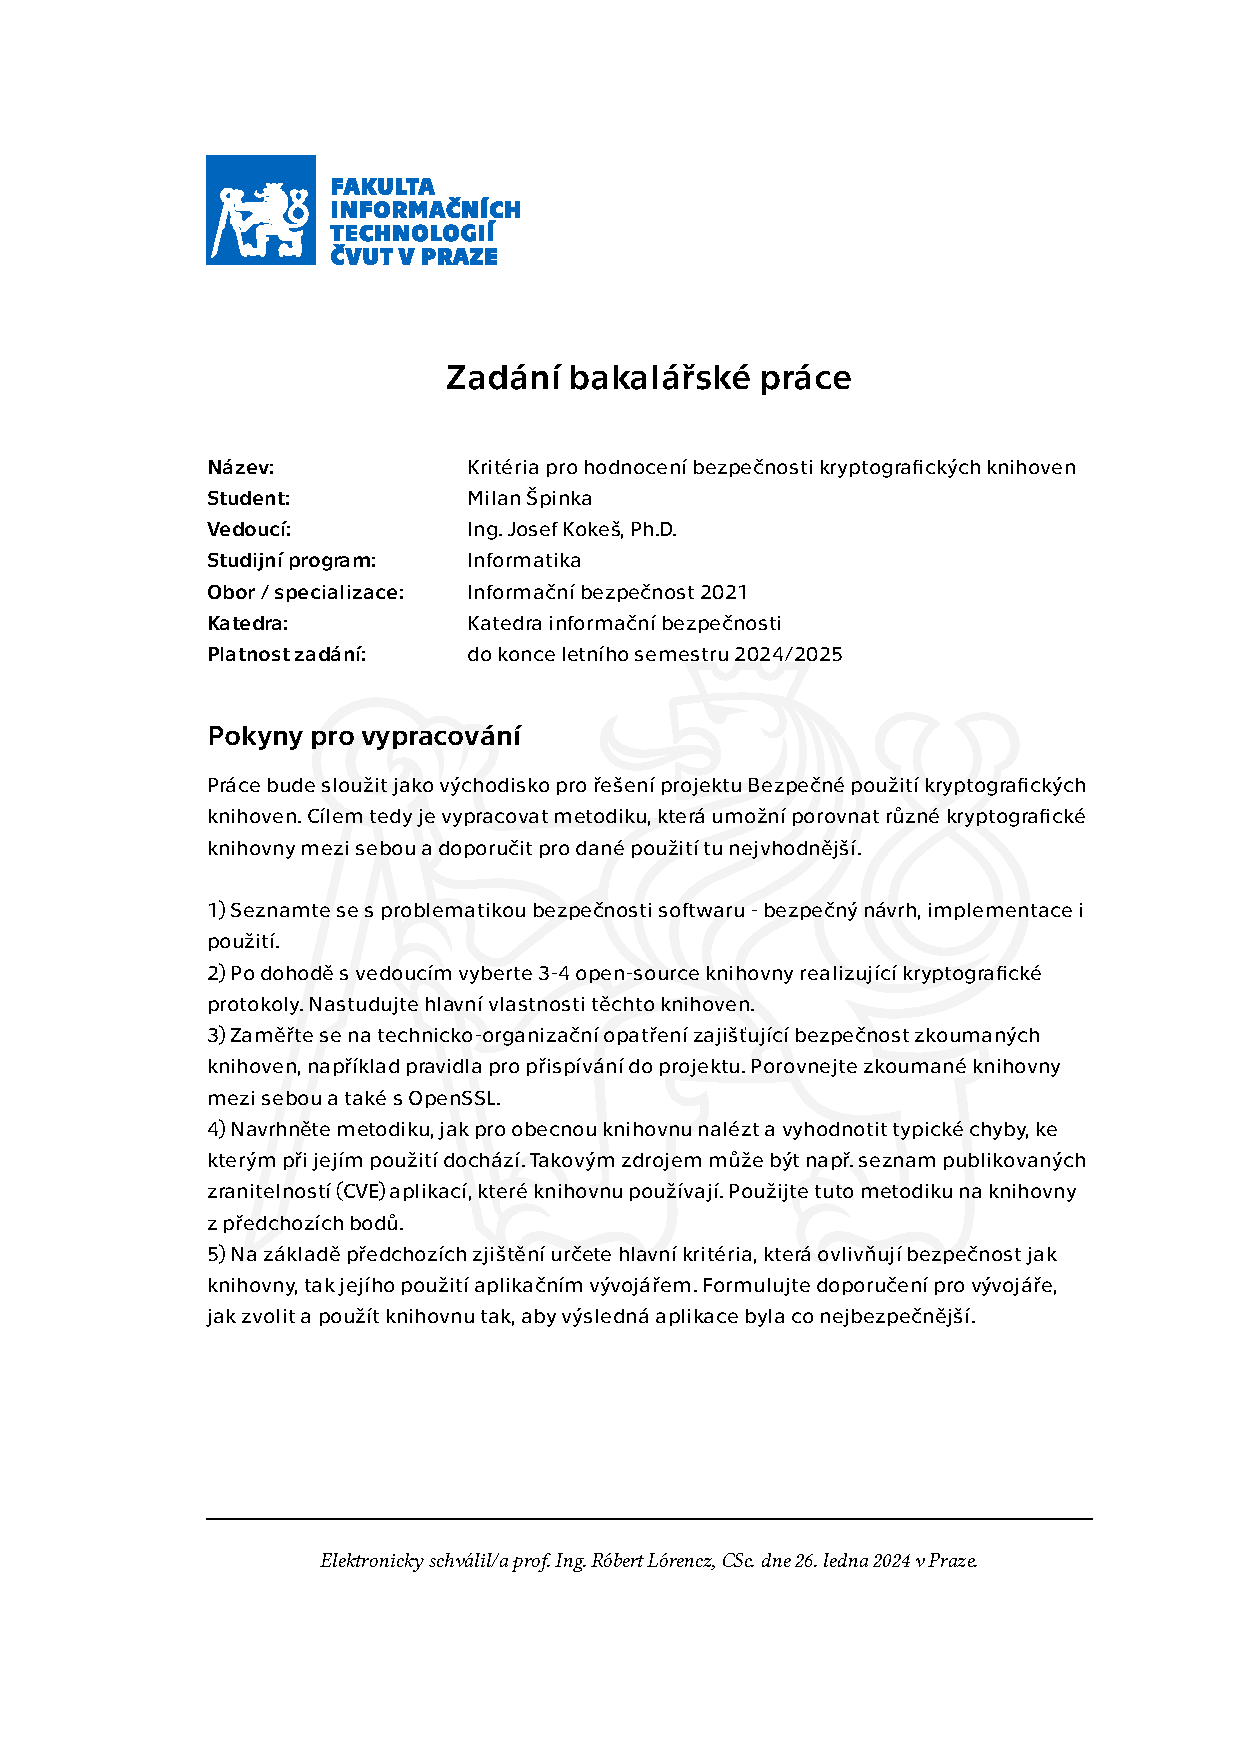
\includepdf[pages={1-}]{spinkmil-assignment.pdf} % replace that file with your thesis assignment provided by study office

\thispagestyle{empty}\cleardoublepage\maketitle % do not remove these three commands

\imprintpage % do not remove this command

\tableofcontents % do not remove this command
%%%%%%%%%%%%%%%%%%%%%%
% list of other contents: figures, tables, code listings, algorithms, etc.
% add/remove commands accordingly
%%%%%%%%%%%%%%%%%%%%%%
\listoffigures % list of figures
\begingroup
\let\clearpage\relax
\listoftables % list of tables
\lstlistoflistings % list of source code listings generated by the listings package
% \listoflistings % list of source code listings generated by the minted package
\endgroup
%%%%%%%%%%%%%%%%%%%%%%
% list of other contents END
%%%%%%%%%%%%%%%%%%%%%%

%%%%%%%%%%%%%%%%%%%
% ACKNOWLEDGMENT
% FILL IN / MODIFY
% This is a place to thank people for helping you. It is common to thank your supervisor.
%%%%%%%%%%%%%%%%%%%
\begin{acknowledgmentpage}
    Chtěl bych poděkovat svému vedoucímu, Ing.\,Josefu Kokešovi,\,Ph.D., za jeho trpělivost, cenné rady, expertízu a~neobvykle pohotový přístup, ale i~za to, že to byl především on, kdo ve mě probudil nadšení pro bezpečný kód a~kryptografii. Dále bych rád poděkoval své rodině a~svým přátelům za jejich přízeň a~podporu nejen v~době vzniku této práce.
\end{acknowledgmentpage} 
%%%%%%%%%%%%%%%%%%%
% ACKNOWLEDGMENT END
%%%%%%%%%%%%%%%%%%%


%%%%%%%%%%%%%%%%%%%
% DECLARATION
% FILL IN / MODIFY
%%%%%%%%%%%%%%%%%%%
% INSTRUCTIONS
% ENG: choose one of approved texts of the declaration. DO NOT CREATE YOUR OWN. Find the approved texts at https://courses.fit.cvut.cz/SFE/download/index.html#_documents (document Declaration for FT in English)
% CZE/SLO: Vyberte jedno z fakultou schvalenych prohlaseni. NEVKLADEJTE VLASTNI TEXT. Schvalena prohlaseni najdete zde: https://courses.fit.cvut.cz/SZZ/dokumenty/index.html#_dokumenty (prohlášení do ZP)
\begin{declarationpage}
Prohlašuji, že jsem předloženou práci vypracoval samostatně a že jsem uvedl veškeré použité informační zdroje v souladu s Metodickým pokynem o dodržování etických principů při přípravě vysokoškolských závěrečných prací. Beru na vědomí, že se na moji práci vztahují práva a povinnosti vyplývající ze zákona č. 121/2000 Sb., autorského zákona, ve znění pozdějších předpisů, zejména skutečnost, že České vysoké učení technické v Praze má právo na uzavření licenční smlouvy o užití této práce jako školního díla podle § 60 odst. 1 citovaného zákona.
\end{declarationpage}
%%%%%%%%%%%%%%%%%%%
% DECLARATION END
%%%%%%%%%%%%%%%%%%%

\printabstractpage % do not remove this command

%%%%%%%%%%%%%%%%%%%
% ABBREVIATIONS
% FILL IN / MODIFY
% OR REMOVE ENTIRELY
% List the abbreviations in lexicographical order.
%%%%%%%%%%%%%%%%%%%
\chapter{Seznam zkratek}
	
\begin{tabular}{rl}
AEAD & \textit{Authenticated Encryption with Associated Data} \\
AES & \textit{Advanced Encryption Standard} \\
API & \textit{Application Programming Interface} \\
CBC & \textit{Cipher Block Chaining} \\
CI & \textit{Continuous Integration} \\
CSPRNG & \textit{Cryptographically Secure Pseudorandom Number Generator} \\
CVE & \textit{Common Vulnerabilities and Exposures} \\
DNS & \textit{Domain Name Service} \\
DSA & \textit{Digital Signature Algorithm} \\
ECB & \textit{Electronic Codebook} \\
ECDH & \textit{Elliptic Curve Diffie-Hellman} \\
ECDSA & \textit{Elliptic Curve Digital Signature Algorithm} \\
EdDSA & \textit{Edwards-curve Digital Signature Algorithm} \\
FFI & \textit{Foreign Function Interface} \\
FIPS & \textit{Federal Information Processing Standard} \\
FLOSS & \textit{Free/Libre and Open Source Software} \\
GCM & \textit{Galois/Counter Mode} \\
GnuPG & \textit{GNU Privacy Guard} \\
HMAC & \textit{Hash-based Message Authentication Code} \\
HTTP & \textit{Hypertext Transfer Protocol} \\
IND-CPA & \textit{Indistinguishability Under Chosen-Plaintext Attack} \\
IV & \textit{Inicializační vektor (Initialization Vector)} \\
JCA & \textit{Java Cryptography Architecture} \\
KDF & \textit{Key Derivation Function} \\
LLM & \textit{Large Language Model} \\
MAC & \textit{Message Authentication Code} \\
MitM & \textit{Man-in-the-middle} \\
NIST & \textit{National Institute of Standards and Technology} \\
OMC & \textit{OpenSSL Management Committee} \\
OSS & \textit{Open Source Software} \\
OTC & \textit{OpenSSL Technical Committee} \\
OT & \textit{Otevřený text (Plaintext)} \\
PBKDF2 & \textit{Password-Based Key Derivation Function 2} \\
PKCS & \textit{Public Key Cryptography Standards} \\
PR & \textit{Pull Request} \\
PyCA & \textit{Python Cryptography Authority} \\
RSA & \textit{Rivest-Shamir-Adleman} \\
SDL & \textit{Secure Development Lifecycle} \\
SHA & \textit{Secure Hashing Algorithm} \\
SSL & \textit{Secure Sockets Layer} \\
SW & \textit{Software} \\
ŠT & \textit{Šifrový text (Ciphertext)} \\
TLS & \textit{Transport Layer Security} \\
\end{tabular}
%%%%%%%%%%%%%%%%%%%
% ABBREVIATIONS END
%%%%%%%%%%%%%%%%%%%

\mainmatter\mainmatterinit % do not remove these two commands

%%%%%%%%%%%%%%%%%%%
% THE THESIS
% MODIFY ANYTHING BELOW THIS LINE
%%%%%%%%%%%%%%%%%%%

%---------------------------------------------------------------%

\chapter*{Úvod}
\addcontentsline{toc}{chapter}{Úvod}\markboth{Úvod}{Úvod}
\setcounter{page}{1}
% ============= %
% Chapter: Úvod %
% Status: Final %
% ============= %

\epigraph{A~little bit of math can accomplish what all the guns and barbed wire can’t: a~little bit of math can keep a~secret.}{E. Snowden, \textit{Permanent Record}, 2019}

Jen velmi těžko si dnes dokážeme představit život ve staroorientálních říších starověké Mezopotámie. Přestože tehdejšího člověka pravděpodobně příliš netrápily otázky ochrany digitálního soukromí, počítačové bezpečnosti nebo open-source kryptografie, můžeme i~tak argumentovat, že už v~tehdejším každodenním životě v~jakési prapůvodní podobě alespoň s~jedním kryptografickým nástrojem do styku přicházel --- tím nástrojem jsou \emph{pečetě}.

Pečeť --- vynález dokonce starší než samotné \textit{písmo} --- byla dlouhá tisíciletí používána kvůli nejméně dvěma užitečným funkcím, které přímo souvisí s~moderní kryptografií. Starší z~nich je tzv.~u\-za\-ví\-ra\-cí funkce. Už ve starověku byly pečetěmi uzavírány např.\ džbány s~vínem nebo olejem, ale i~místnosti nebo domy. Praktičnost takového použití pečetí spočívala v~jeho schopnosti prokázat \emph{integritu} uzavíraného objektu --- dokud byla pečeť na džbánu s~vínem neporušená, mohli jste předpokládat, že s~obsahem džbánu nebylo manipulováno a~víno není třeba otrávené; jakmile jste do džbánu vnikli, zanechali jste nevratnou, viditelnou stopu.~\cite{sfragistika}

Druhou podstatnou funkcí pečetě byla funkce ověřovací, kterou hojně využívali panovníci a~státní aparáty. Když například sicilský král Fridrich II.\ v~roce 1212 českému králi Přemyslu Otakarovi~I.\ udělil privilegium dědičnosti jeho titulu, opatřil slavnou listinu provádějící tento akt pečetí ze zlata (neboli zlatou bulou), kterou jednoznačně zaručil její \emph{autenticitu}.~\cite{sfragistika, zlatabula}

S~rozvojem gramotnosti v~západní společnosti byly pečetě nakonec nahrazeny razítky a~vlastnoručními podpisy, které pro ověření právních dokumentů používáme dodnes. Tyto nástroje mají ale jednu nevýhodu --- nelze je dobře použít pro ověřování digitálních dat. Řešením je zcela nový ověřovací prostředek založený na asymetrické kryptografii, totiž \emph{digitální podpis}.

Všechny zmíněné prostředky pro ověřování pravosti dokumentů jsou postavené na témže předpokladu, že nemohou být (jednoduše) zfalšovány. Zatímco pečetě a~podpisy se spoléhají v~nějakém smyslu na nezfalšovatelnost fyzickou, digitální podpisy stojí zpravidla na matematickém problému, který lidstvo nedokáže bez znalosti tajného klíče efektivně vyřešit, například faktorizaci\footnote{Tj.~rozklad složeného čísla na jeho prvočíselné dělitele.} velmi velkých čísel nebo tzv.~problému diskrétního logaritmu. To z~nich činí mocný nástroj --- nezáleží na tom, kolik peněz a~technických prostředků máte, jestli jste prezident nebo diktátor; pokud neobjevíte převratný algoritmus, který by složitost daného matematického problému prolomil, podpis nezfalšujete.

Vedle integrity a~autenticity zpráv si kryptografie dává za cíl zajistit ještě jednu velmi žádanou vlastnost komunikace, kterou je její \emph{důvěrnost}. Důvěrnost zprávy jednoduše znamená její nesrozumitelnost pro neoprávněnou třetí stranu a~dosahuje se jí typicky nějakým druhem šifrování. Historická motivace pro studium šifer vychází z~vojenství --- římští císaři používali pro komunikování se svými generály jednoduché substituční šifry, notoricky známá je Caesarova šifra, která nahradí každý znak zprávy znakem, který je v~latinské abecedě o~3~místa dál (A se přepíše na D, B na E, atd.); další proslulou šifrou je Enigma, za druhé světové války používaná nacistickým Německem, k~jejímuž vyluštění přispěl stroj, který je dnes považován za předchůdce moderních počítačů. Obzvlášť v~dnešní době je ale šifrování používáno i~mimo vojenství a~diplomacii jako prostředek pro zabezpečení digitální komunikace, ochranu osobních dat, digitálního soukromí, obchodních tajemství, apod. \cite{kahn1996codebreakers}

Cílem předchozích odstavců bylo především vyzdvihnout skutečnost, že problémy, které kryptografie řeší, nejsou nikterak složité nebo nové --- nové je jen to, že místo kovových pečetí, zámků z~oceli a~strojů Enigma používáme k~utajení a~zabezpečení informací a~digitální komunikace nástroje, které nám dává algebra, teorie čísel a~další oblasti moderní matematiky. Použití matematické kryptografie pro zabezpečení informačních a~komunikačních systémů s~sebou ale kromě silných bezpečnostních záruk nese i~jednu nevýhodu: Kryptografie je složitá~\cite{youreallyshouldnt, hurdles}. Navrhnout kryptografický protokol nebo algoritmus tak, aby byl skutečně bezpečný a~poskytoval záruky, které od kryptografie očekáváme, není zdaleka jednoduché a~vyžaduje dalekosáhlou expertízu. To přirozeně vede k~jisté nerovnováze: V~době internetu a~digitální komunikace nelze potřebu kryptografie přecenit --- téměř jakákoli webová aplikace dnes musí používat kryptografické protokoly\footnote{Čtenář je jistě přinejmenším z~uživatelského hlediska obeznámen s~protokolem HTTPS, který spočívá v~obalení HTTP komunikace kryptografickým protokolem TLS.}, aby ochránila své uživatele před nemilosrdnými útočníky, kteří na internetu číhají. Takových aplikací přitom mohou být miliony~\cite{appstorestats} a~uživatelů, jejichž soukromí a~bezpečí závisí na kvalitní kryptografii, potenciálně ještě více. Oproti tomu expertů, kteří jsou takové kvalitní kryptografické algoritmy a~protokoly schopní navrhnout, je relativně málo.

V~praxi je tento problém řešen skrze standardizaci kryptografických algoritmů a~jejich otev\-ře\-nou im\-ple\-men\-ta\-ci v~\emph{kryptografických knihovnách}\footnote{Softwarová knihovna je jednoduše kód, který řeší nějakým způsobem často používanou funkcionalitu a~může být proto opětovně používán napříč programy.}.
Kryptografické algoritmy (resp.\ protokoly) na\-vr\-že\-né experty jsou podrobeny recenzi vědecké komunity a~v~případě, že se osvědčí jako bezpečné, standardizovány nějakou standardizační autoritou (např. \textit{Internet Engineering Task Force}, IETF). Zveřejněné algoritmy pak může kdokoli implementovat v~nějakém programovacím jazyce a~z\-ve\-řej\-nit je jako součást kryptografické knihovny. Aplikační vývojáři tak v~důsledku nemusí algoritmus sami programovat, ale mohou použít některou dostupnou implementaci.

Výše popsaný model není ani mimo oblast kryptografie v~softwarovém vývoji nic neobvyklého; až 96 \% dnešního softwaru nějakým způsobem na takových sdílených knihovnách závisí~\cite{synopsysossreport}. Přirozenou otázkou může --- a~mělo by --- být, kdo takové veřejně dostupné implementace tvoří a~jestli jejich autorům opravdu můžeme věřit, že je tvoří správně a~bezpečně. Relevanci takové otázky podtrhuje bezpečnostní incident z~letošního března, kdy byla nalezena zadní vrátka\footnote{Zadní vrátka, angl.\ \textit{backdoor}, je označení pro mechanismus, který výlučně jeho autorovi dovoluje později obejít bezpečnostní mechanismy daného systému.} v~populárním (až všudypřítomném) softwarovém balíčku \texttt{xz-utils}~\cite{cve-2024-3094}, která byla pravděpodobně do tohoto softwaru umístěna záměrně jedním z~jeho vývojářů.

Často slýchaný argument, který by použil dogmatický zastánce open-source kódu, tvrdí, že pokud je kód knihovny dostupný veřejně všem, pak se zákonitě najde někdo, kdo má dostatečné kompetence v~oboru informační bezpečnosti (případně i~zájem na tom, aby byl produkt bezpečný), zdrojový kód si přečte, zhodnotí jej a~případně upozorní na jeho bezpečnostní nedostatky\footnote{Ostatně \emph{v~nějakém smyslu} podobným způsobem byl objeven i~zmíněný backdoor v~\texttt{xz-utils}~\cite{vergexz}.}. S~takovým argumentem se lze ale z~pozice bezpečnostního analytika jen těžko spokojit, obzvlášť pak v~případě, že předmětem zkoumání je populární kryptografická knihovna, na jejímž kódu potenciálně závisí soukromí a~bezpečí milionů uživatelů.

Jeví se proto jako vysoce žádoucí nalézt obecnou metodu, na základě které by bylo možné s~rozumným úsilím a~nestranností zhodnotit kvalitu, bezpečnost a~důvěryhodnost dané knihovny a~rozhodnout, jestli má nebo nemá být v~projektu použita, případně pod jakými podmínkami. To je \textit{raison d'être} této práce.

\begin{figure}
    \centering
    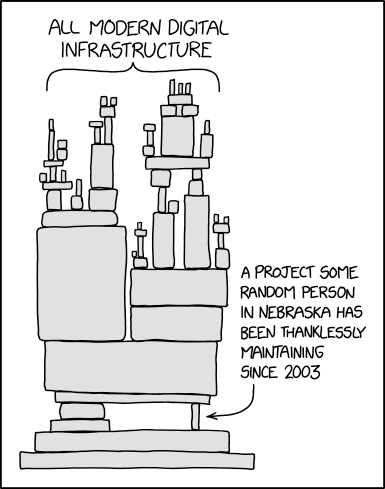
\includegraphics[width=0.5\textwidth]{text/media/dependency.png}
    \caption[~Komiks umělce xkcd s~názvem ``\textit{Dependency}'']{Komiks umělce xkcd z~roku 2020 s~názvem ``\textit{Dependency}'' ilustruje křehkost používání závislostí ve vývoji softwaru.~\cite{xkcd}}
\end{figure}

\section*{Cíle práce}\addcontentsline{toc}{section}{Cíle práce}\markboth{Cíle práce}{Cíle práce}

Jedním z~předních motivů pro vznik této práce byla účast na řešení výzkumného projektu Národního úřadu pro kybernetickou a~informační bezpečnost, který se zabýval hodnocením bezpečnosti open-source kryptografických knihoven a~identifikací rizik jejich používání --- k~řešení tohoto projektu přispívají i~bakalářské práce Matěje Douši~\cite{matej} a~Kirilla Leonova~\cite{kirill}. Cíle této práce, z~velké části kopírujíce cíle zmíněného projektu, zahrnují:

\begin{enumerate}
    
    \item provést rešerši dostupných informací o~možných způsobech hodnocení bezpečnosti open-source kryptografických knihoven, případně bezpečnosti pouze open-source knihoven, pouze kryptografických knihoven nebo softwaru obecně;

    \item navrhnout způsob, jak pro danou kryptografickou knihovnu identifikovat časté chyby nebo nepochopení, se kterými se uživatelé při práci s~ní potýkají;

    \item na základě těchto zjištění formulovat sadu kritérií, podle kterých bude s~rozumným úsilím možné zhodnotit knihovnu a~případně doporučit nebo nedoporučit její použití;

    \item na vybraných open-source kryptografických knihovnách demonstrovat získané výsledky.
    
\end{enumerate}

Potřeba takové metodiky vychází z~pozorování, že se nejeví jako proveditelné, aby každá verze každé jednotlivé knihovny implementující kryptografické algoritmy byla kompletně bezpečnostně auditována a~otestována. Zaprvé by šlo o~aktivitu tak časově, kognitivně a~ekonomicky náročnou, že by jen málokdy připadala v~úvahu, zadruhé takový postup nelze aplikovat, pokud analytik nedisponuje potřebnou expertízou. Nakonec by ani takový přístup nemusel nutně pokrýt všechny aspekty bezpečnosti knihovny, jako například pravděpodobnost, že ji i~další uživatel, který nezná detailně její vnitřní fungování, bude schopný správně použít.

Text této práce je dále organizován následujícím způsobem. Kapitoly~\ref{software} a~\ref{pouziti} uvedou čtenáře do problematiky bezpečnosti softwaru, resp.\ zranitelného použití kryptografie a~jeho předcházení, a~shrnou vědecké poznatky v~těchto oblastech. V~kapitole~\ref{analyza} popíšeme vybrané kryptografické knihovny a~provedeme analýzu jejich relevantních vlastností. Výslednou metodu pro hodnocení bezpečnosti kryptografických knihoven popíšeme v~kapitole~\ref{vysledky} a~výsledky práce shrneme v~závěrečné kapitole~\ref{zaver}.


%---------------------------------------------------------------%

\chapter{Bezpečnost softwaru}
% ============================ %
% Chapter: Bezpečnost softwaru %
% Status: Final                %
% ============================ %
\label{software}

Kryptografické knihovny spadají --- stejně jako spustitelné programy nebo webové aplikace --- pod obecnou definici softwaru. I~přes jejich mnohá specifika se na ně proto vztahují obecné poznatky o~bezpečnosti softwaru, které představíme v~této kapitole. Vzhledem k~tomu, že kód kryptografických knihoven je navíc zpravidla veřejný (tzv.~\textit{open-source}), věnujeme zvláštní pozornost právě takto vyvíjenému a~publikovanému softwaru.

V~rámci této kapitoly definujeme klíčové pojmy, popíšeme tradiční přístupy k~bez\-peč\-né\-mu vývoji softwaru, a~následně provedeme rešerši literatury týkající se bezpečnosti open-source softwarových projektů a~jejich vývoje.

\section{Definice}

Bezpečnost softwaru (SW) je poměrně široký a~volně interpretovatelný pojem, je proto důležité ho --- alespoň pro účely této práce --- přesně vymezit. V~tomto textu vyjdeme především z~práce autorů D.~LeBlanca a~M.~Howarda~\cite{leblanc2002writing} a~jejich definic založených na \emph{CIA modelu}. Akronym CIA v~sobě zahrnuje tři žádoucí vlastnosti chráněného systému, totiž jeho důvěrnost (C --- \textit{confidentiality}), integritu (I --- \textit{integrity}) a~dostupnost (A --- \textit{availability}).

\begin{definition}[Bezpečnostní zranitelnost]
    Bezpečnostní zranitelnost v~softwaru (dále jen zranitelnost) je jakýkoli jeho nedostatek, který umožňuje útočníkovi získat neoprávněný přístup k~uživatelově systému, poškodit data v~něm nebo zamezit jeho fungování. \cite{leblanc2002writing}
\end{definition}

\begin{definition}[Bezpečný software]
    Bezpečný je takový software, který zajišťuje důvěrnost, integritu a~dostupnost uživatelských dat a~zároveň integritu a~dostupnost výpočetních prostředků vlastníka nebo administrátora systému. \cite{leblanc2002writing}
\end{definition}

Objevené softwarové zranitelnosti jsou zpravidla publikovány skrze projekt \textit{Common Vulnerabilities and Exposures} (CVE), který spravuje sdílenou databázi zranitelností a~je de~facto mezinárodním standardem pro identifikaci zranitelností~\cite{cve-overview}. Kromě unikátního identifikátoru (CVE ID), který má právo udělit kterákoli z~partnerských organizací projektu CVE, je zranitelnostem často přidělováno hodnocení \textit{Common Vulnerability Scoring System} (CVSS), které na škále od 0 do 10 hodnotí závažnost dané zranitelnosti, a~v~některých případech identifikátor \textit{Common Weakness Enumeration} (CWE), který charakterizuje druh (programátorské, konfigurační, apod.) chyby, která danou zranitelnost zapříčinila.

\section{Strategie pro zabezpečení softwaru}

V~následující části popíšeme některé způsoby, kterými lze software zabezpečit, tj.\ odstranit jeho zranitelnosti nebo ještě lépe jejich vzniku už při samotném vývoji předcházet.

LeBlanc a~Howard \cite{leblanc2002writing} doporučují vývojářským týmům k~bezpečnosti přistupovat proaktivně. Argumentují, že pokud se vývojáři nebudou zajímat o~bezpečný vývoj softwaru, pak jej nebudou vyvíjet bezpečně; podobně pokud nebudou organizační procesy spjaté s~vývojem zahrnovat bezpečnostní praktiky, výsledný produkt nebude bezpečný. Společnost Microsoft tento přístup implementuje skrz strategii SD\textsuperscript{3} a~framework \textit{Secure Development Lifecycle} (SDL)~\cite{mssdl}.

\subsection{\texorpdfstring{SD\textsuperscript{3}}{SD3}}

Strategie SD\textsuperscript{3} sestává ze tří imperativů: Software má být bezpečný ve svém návrhu (\textit{secure by design}), ve svém výchozím nastavení (\textit{secure by default}) a~má umožňovat snadnou a~bezpečnou údržbu (\textit{secure in deployment}).~\cite{leblanc2002writing}

\subsubsection*{Bezpečný návrh}

První imperativ vychází z~poznatku, že je jednodušší zabezpečit software, který je už od začátku navržen s~ohledem na bezpečnost, než ad hoc způsobem opravovat zranitelnosti ve špatně na\-vr\-že\-ném softwaru. V~týmu vývojářů by proto měla být dedikovaná osoba dohlížející na (a~zodpovídající za) bezpečnost produktu; spolu s~návrhem softwaru by měl být popsán model hrozeb a~produkt by měl být alespoň před zveřejněním bezpečnostně otestován.

\subsubsection*{Bezpečný výchozí stav}

Výchozí nastavení softwaru má být bezpečné z~prostého důvodu, že většina jeho uživatelů půjde cestou nejmenšího odporu a~zvolí právě ta nastavení, která jsou v~softwaru výchozí. (To platí nejen o~koncových uživatelích programů, ale i~o~vývojářích používajících open-source knihovny, jak uvidíme později v~této práci.) Proto se doporučuje ve výchozím stavu ponechat pouze minimální počet maximálně bezpečných funkcionalit a~zbytek případně nechat uživatele doinstalovat nebo je poskytnout v~režimu \emph{opt-in}.

\subsubsection*{Bezpečná údržba}

Poslední pravidlo vychází z~pozorování, že prakticky žádný netriviální software není bezchybný --- v~každém programu nebo knihovně bude dříve nebo později nalezena chyba s~potenciálními bezpečnostními dopady, a~i~kdyby ne, úkolem bezpečného vývoje softwaru je s~takovou možností počítat. Proto je potřeba zajistit jednoduchý, spolehlivý a~bezpečný mechanismus, jak k~u\-ži\-va\-te\-lům dopravit nové verze s~opravenými zranitelnostmi.

\subsection{Secure Development Lifecycle}

Metodika SDL částečně vychází z~SD\textsuperscript{3} a~představuje strategii pro vývoj softwaru, v~níž je důraz na bezpečnost produktu kladen už od počátečního návrhu. SDL za tímto účelem definuje 12~bezpečnostních praktik, které je v~průběhu vývoje (ale i~před jeho začátkem a~po jeho ukončení, resp.\ po vydání softwaru) třeba dodržovat.~\cite{mssdl}

Před samotným začátkem vývoje radí SDL seznámit členy vývojářského týmu (včetně softwarových architektů, produktových manažerů, atd.) se základní problematikou bezpečnosti softwaru, tj.\ s~cíli a~způsobem přemýšlení útočníků. Dále radí definovat bezpečnostní požadavky a~metriky pro jejich pozdější měření a~hodnocení. Až poté mají být navrženy požadavky na funkce softwaru a~na jejich základě navržen model hrozeb (\textit{threat model}).

Doporučení modelu SDL se stručně dotýkají i~používání kryptografie a~rizik plynoucích z~použití softwarových závislostí: Volba kryptografických standardů použitých pro zabezpečení dat a~komunikace má být ponechána na expertech a~pro jejich implementaci má být zvolena knihovna, která bude v~případě potíží nebo vzniku bezpečnostního incidentu snadno nahraditelná. Dále SDL radí řídit obecná rizika spojená s~použitím závislostí třetích stran, přičemž se odkazuje např.\ na návod publikovaný projektem SAFECode~\cite{safecodetpc}.

Co se týče samotného procesu vývoje SW, vyžaduje SDL stanovení seznamu schválených nástrojů pro vývoj, tzn.\ překladačů a~jejich přepínačů (např.\ přísný režim kompilace), statických analyzátorů, nástrojů pro modelování hrozeb, atd. V~průběhu vývoje mají být používány techniky statické a~dynamické analýzy kódu a~před vydáním softwaru má být proveden penetrační test.

Posledním aspektem bezpečného vývoje jsou reakce na nově objevené bezpečnostní problémy (\textit{incident response}). Model SDL požaduje určit kontaktní osobu pro nahlašování incidentů a~vytvořit plán pro reakci na různé typy incidentů (včetně zranitelností v~softwaru třetích stran).

\subsection{Další bezpečnostní principy}

Kromě konkrétních strategií LeBlanc a~Howard~\cite{leblanc2002writing} popisují několik obecných bezpečnostních principů, kterými je vhodné se při vývoji softwaru řídit. Patří mezi ně mimo jiné:

\begin{itemize}
    \item \textbf{Víceúrovňová bezpečnost} (někdy též \emph{vrstvená bezpečnost}, angl.\ \textit{defence in depth}): Tento princip tvrdí, že každý ochranný prvek jednou selže a~proto bychom se neměli spoléhat pouze na jeden bezpečnostní mechanismus, ale kombinovat jich několik.

    \item \textbf{Odmítnutí bezpečnosti skrze neznalost} (angl.\ \textit{security through obscurity}): Útočníkova neznalost systému nesmí být jediným prostředkem jeho zabezpečení. Skrytí implementace bezpečnostních mechanismů může jejich prolomení ztížit, samotné k~jejímu zabezpečení ale nestačí.

    \item \textbf{Selhání do bezpečného módu}: Pokud v~softwaru dojde k~chybě, její ošetření by mělo být bezpečné. Reakce na chybu by navíc neměla zbytečně prozradit příliš mnoho informací (příkladem zneužití takové slabiny je například \textit{padding oracle attack} na protokol TLS~\cite{cloudflarepaddingoracle}).
\end{itemize}

\section{Open-source a closed-source software}

Poznatky z~předchozích odstavců jsou aplikovatelné na libovolný software, v~této práci budeme ale věnovat speciální pozornost bezpečnosti a~bezpečnému vývoji především jedné konkrétní třídy softwaru, který budeme označovat jako open-source a~který nyní definujeme.

\subsubsection*{Open-source software}

Pod anglickým termínem \emph{Open-Source Software} (OSS), česky \emph{software s~otevřeným zdrojovým kódem}, se obecně rozumí software, jehož zdrojový kód je publikovaný a~veřejně přístupný (zpravidla na internetu). Často je takový software bezplatný a~dovoluje uživatelům ho volně modifikovat a~redistribuovat~\cite{schryen2009security}, to se ale odvíjí od licence, pod kterou autoři svůj kód zveřejní, a~samo o~sobě nesouvisí s~tím, jestli je zdrojový kód veřejně přístupný. V~užším smyslu lze open-source software chápat také jako software splňující definici organizace Open Source Initiative, která kromě otevřeného zdrojového kódu od daného softwaru vyžaduje mimo jiné licenci dovolující jeho neomezenou a~bezplatnou redistribuci a~modifikaci~\cite{osidefinition}. Software splňující tuto definici je často označován jako Free Open-Source Software (FOSS, příp.\ FLOSS\footnote{Písmeno L v~akronymu FLOSS označuje francouzské slovo \textit{libre}, které má ujasňovat, že pojmem \emph{free software} se rozumí nikoli bezplatný software, ale \emph{svobodný} software.}.).

Jednoznačně nejprominentnějším přínosem OSS v~dnešní době je ekonomická výhodnost jeho použití~\cite{boughton2024decomposing} --- vývojáři softwaru nemusí sami implementovat a~testovat každou funkci, kterou jejich program vyžaduje, ale mohou využít open-source implementace běžných komponent, jako je třeba webový server nebo knihovna pro manipulaci s~obrazovými daty. Průzkumy z~roku 2017 ukázaly, že na otevřeném kódu celosvětově závisí až 96~\% aplikací a~80~\% obchodních společností~\cite{wen2019security}. Přirozeným záporem použití open-source softwaru je nevyhnutelná skutečnost, že tím vývojář přistupuje na \emph{trust contract} vůči správcům této závislosti, neboli vědomě přijímá rizika, která z~použití cizího kódu plynou~\cite{boughton2024decomposing}.

\subsubsection*{Closed-source software}

Closed-source software je software, který není open-source, tzn.\ jeho zdrojový kód není veřejně přístupný. Closed-source software může a~nemusí být zpoplatněný a~typicky je distribuovaný v~podobě spustitelného binárního souboru~\cite{schryen2009security}.

Častým omylem je domněnka, že u~closed-source programu si uživatel nemá možnost ``přečíst kód''. Ve skutečnosti má technicky znalý uživatel i~v~případě closed-source software možnost kód analyzovat pomocí technik disassemblování, příp.\ dekompilace. Problém s~tímto přístupem je, že výsledkem takového procesu může být kód na velmi nízké úrovni abstrakce (například strojový kód procesoru nebo bytecode interpretovatelný virtuálním strojem) a~navíc může být program záměrně obfuskovaný, aby porozumění jeho kódu bylo co nejobtížnější. Bezpochyby je analýza closed-source softwaru mnohem složitější a~technicky náročnější než analýza otevřeného kódu, není však nemožná.

\section{Bezpečnost open-source softwaru}

S~open-source softwarem se kromě otevřeného zdrojového kódu a~permisivních licencí pojí i~další specifika. Oproti ``konvenčním'' modelům vývoje softwaru jsou open-source projekty rozmanitější, co se týče různých typů vývojových procesů~\cite{scacchi2006understanding}. Vývoj open-source softwaru často probíhá distribuovaně a~podílí se na něm velký počet vývojářů, kteří pocházejí z~rozmanitých prostředí a~disponují různými úrovněmi expertízy~\cite{wen2019security}. Takový model vývoje OSS bývá označován jako ``tržištní'' a~je stavěn do kontrastu s~vývojem ``katedrálovým'', ve kterém se na vývoji podílí pouze malá, ale organizovaná skupina vývojářů~\cite{raymond1999cathedral}.

Tržištní model, v~němž na vývoji softwaru spolupracují lidé z~celého světa, s~sebou ale přináší nové výzvy s~ohledem na bezpečnost. Důvěryhodnost open-source projektů závisí na různých so\-ci\-ál\-ně-tech\-nic\-kých aspektech vývoje, jako je expertíza vývojářů, kvalita použitých nástrojů, důk\-lad\-nost testovacích procesů a~bezpečná integrace nového kódu~\cite{oss-security-literature}, přičemž tyto aspekty je náročnější v~takovém modelu zajistit. Výzkum dále poukazuje na ne\-dos\-ta\-teč\-nou organizaci znalostí v~open-source projektech, která může být problematická v~kontextu toho, že přispěvatelé do OSS zaprvé nemusí mít potřebné znalosti pro identifikaci bezpečnostních rizik a~zadruhé bezpečnost nebývá jejich hlavním zájmem~\cite{wen2019security}.

Vzhledem ke kritické roli otevřeného kódu v~dnešním světě a~specifikům vývojového procesu v~open-source projektech je přirozené se ptát, nakolik je takto vyvíjený software bezpečný, případně co k~jeho bezpečnosti přispívá, nebo jí naopak škodí.

\subsection{Open-source vs. closed-source}

Otázka, kterou se akademická debata zabývala především v~nultých letech, míří na porovnání bezpečnosti open-source a~closed-source softwaru s~cílem zjistit, jestli je jeden přístup inherentně bezpečnější než druhý~\cite{oss-security-literature}.

Notorickým argumentem příznivců open-source je myšlenka, která bývá označována jako \emph{Linusův zákon}~\cite{osslinuslaw2014}. Tento termín zavedl americký programátor Eric Raymond, který v~eseji \emph{Katedrála a~tržiště} z~roku~2001 píše, že ``\textit{pokud máte dostatek očí, všechny chyby jsou průhledné}''~\cite{raymond1999cathedral}. Tím chce v~zásadě říct, že pokud je kód programu dostupný veřejně všem, pak se jistě najde dostatek lidí s~příslušnou expertízou, kteří si kód přečtou a~najdou v~něm případné chyby.

Druhá strana debaty je k~této myšlence skeptická. Někteří jí oponují ve smyslu argumentu ``\textit{Ano, zdrojový kód je dostupný všem, ale čte ho někdo?}''~\cite{open-vs-closed}, jiní se odkazují na sociálně-psychologický jev \emph{difúze odpovědnosti} a~namítají, že představa Linusova zákona může v~mnoha potenciálních recenzentech kódu vyvolat dojem, že kód revidoval už někdo jiný, a~tím pádem to není potřeba dělat~\cite{osslinuslaw2014}. V~neposlední řadě se nabízí argument, že zatímco o~bezpečnostních analyticích Linusův zákon s~nadsázkou předpokládá, že budou kód studovat z~dobroty srdce, u~skutečných útočníků si můžeme být jistí, že jejich motivace veřejný kód studovat bude mnohem konkrétnější --- totiž nalezené chyby, které mohou zneužít pro vlastní zisk.

Z~literární rešerše nevyplynulo žádné důvodné podezření, že by open-source software měl být z~principu bezpečnější než closed-source software, nebo naopak. Schryen~\cite{schryen2009security-debate} například uvádí, že ``\textit{se obě strany [debaty] shodují na tom, že otevřený kód usnadňuje nalézání zranitelností, neshodují se ale na tom, jaký to má vliv na bezpečnost}''. Schryen a~Kadura~\cite{open-vs-closed} poukazují na to, že v~jistém smyslu lze debatu redukovat na problém bezpečnosti skrze neznalost, kterou lze dosledovat až ke Kerckhoffsově publikaci \emph{La cryptographie militaire}~\cite{kerckhoffs1883cryptographie} z~roku~1883.

\subsection{Indikátory bezpečnosti open-source kódu}

Přestože akademická debata o~(ne)bezpečnosti open-source softwaru nepřinesla konkrétní závěry, podle reportu organizace MITRE se už v~roce~2006 federální vláda Spojených států amerických v~rámci své kritické infrastruktury spoléhala na více než 200 open-source balíčků~\cite{dhsbacksoss}. Dá se tedy předpokládat, že open-source software byl veřejností přijat jako srovnatelně bezpečný jako closed-source software, čemuž nasvědčuje dodnes pokračující trend adopce open-source softwaru soukromým i~veřejným sektorem.

Novější literatura (cca od roku 2009 dál) se častěji věnuje konkrétním aspektům, které ovlivňují bezpečnost OSS. Empirický výzkum z~let 2011--2014~\cite{oss2011, osslinuslaw2014} ukazuje, že Linusův zákon ve vztahu k~bezpečnostním zranitelnostem obecně neplatí a~dokonce v~jistém smyslu \emph{odporuje} pozorované skutečnosti.

Článek~\cite{oss2011} z~roku~2011 představuje model, který na základě statistik jednotlivých souborů kódu dokáže s~vysokou úspěšností ($>$~80~\%) predikovat, které soubory obsahují zranitelný kód. Prediktory autoři rozdělují do tří kategorií: složitost kódu, míchání kódu\footnote{V~angl.\ originále \emph{code churn}.} a~aktivita vývojářů. Výsledky demonstrují na dvou velkých open-source projektech, prohlížeči Mozilla Firefox a~jádře operačního systému Red Hat Enterprise Linux (RHEL).

\begin{itemize}
    \item \textbf{Složitost kódu:} \enskip
        Napříč akademickou debatou panuje shoda, že složitost systémů je vý\-znam\-ným rizikem pro jejich bezpečnost~\cite{youreallyshouldnt, oss2011, impact-openssl}. Složitý kód se hůře spravuje, čte a~testuje~\cite{mccabe1976complexity} a~je proto očekávatelné, že s~rostoucí složitostí kódu bude růst počet chyb a~tedy i~zranitelností. To potvrzují i~empirické výsledky, podle nichž pozitivně koreluje se zranitelnostmi mj.\ počet řádků kódu v~souboru, počet deklarací a~definovaných funkcí, cyklomatická složitost kódu, maximální úroveň vnoření kódu nebo také počet vstupních a~výstupních parametrů funkcí.
    \item \textbf{Míchání kódu:} \enskip
        Tato kategorie metrik vychází ze zjištění~\cite{nagappan2005use, graves2000predicting}, že s~každou změnou v~kódu roste riziko vzniku zranitelnosti. Použité metriky měří, kolik jednotek změn (commitů) a~řádků změn soubor čítá od svého vzniku a~podobně kolik řádků kódu bylo do souboru od jeho vzniku kumulativně přidáno. Všechny tři metriky v~obou projektech pozitivně korelují se zranitelným kódem.
    \item \textbf{Aktivita vývojářů:} \enskip
        Zranitelný kód byl častěji obsažen v~souborech obsahujících kód vět\-ší\-ho počtu vývojářů. Dále byl častěji zranitelný kód, do kterého přispívali vývojáři, kteří zá\-ro\-veň přispívali do mnoha dalších částí projektu. Jako poslední se ukázalo být rizikové, když do kódu přispívali vývojáři, kteří nebyli pro síť přispěvatelů ``centrální''\footnote{Síť vývojářů je definovaná jako neorientovaný graf: Vrcholy v~něm odpovídají jednotlivým vývojářům a~mezi dvěma vrcholy je hrana právě tehdy, když oba odpovídající vývojáři přispěli alespoň do jednoho společného souboru. Centralita vývojáře v~síti je popsána několika metrikami, jednou z~nich je např.\ stupeň vrcholu.}.
\end{itemize}

Na popsanou studii navazuje o~tři roky později publikovaný článek \cite{osslinuslaw2014}, který přímo adresuje Linusův zákon a~na open-source projektu Chromium zkoumá vliv důkladnosti revize kódu a~míry ``sociálně-technické obeznámenosti'' vývojářů s~projektem na výskyt zranitelností ve vydaných verzích. Kromě zjištění konzistentních s~předchozím výzkumem došli autoři k~dalším překvapivým výsledkům:

\begin{itemize}
    \item \textbf{Počet recenzentů změn:} \enskip
        Soubory se zranitelným kódem revidovalo více lidí (přepočteno na řádku kódu), konkrétně revize od 3 a~více lidí vedla k~zvýšení rizika výskytu zranitelnosti téměř dvakrát. Autoři tuto metriku zvolili na základě oficiálních doporučení pro přispívání do projektu Chromium, která vycházejí ze ``\textit{zkušenosti, že kdykoli kód revidují 3 nebo více recenzentů, dochází k~nejasnostem ohledně toho, kdo má v~procesu jakou roli}''~\cite{osslinuslaw2014}.
        
        Tento výsledek silně rozporuje tvrzení Linusova zákona a~podporuje argument o~difúzi odpovědnosti. Otázkou zůstává, jestli se dá vztáhnout na open-source projekty obecně, nebo jestli je způsoben nějakým neznámým specifikem projektu Chromium.

    \item \textbf{Účastníci diskuzí nad změnami:} \enskip
        Do diskuzí nad zranitelným kódem se zapojovalo celkově více lidí, zároveň se ale méně často zapojili účastníci se zkušenostmi se zranitelným kódem a~jeho opravami. Autoři toto zjištění podkládají přesvědčivou argumentací --- namítají, že v~projektu Chromium se zranitelnost vyskytla jen v~necelých 5~\% souborů, což znamená, že průměrný vývojář se nemusel vůbec za dobu svého působení v~projektu se zranitelným kódem potkat a~v~důsledku nemusí mít dostatečnou expertízu k~jeho odhalení, i~když se revize zúčastní. K~podobným závěrům, tedy že vývojáři často nejsou dostatečně kvalifikovaní na to, aby odhalili bezpečnostní problémy v~kódu, došli i~další akademici~\cite{wen2019security, open-vs-closed}. Zároveň ve světle takového argumentu nepůsobí tak neintuitivně zjištění jiné studie, že zkušenější vývojáři častěji přispívají zranitelným kódem, než vývojáři méně zkušení~\cite{bosu2014characteristics}. Z~těchto důvodů je podle autorů potřeba, aby se do revizí zapojovali účastníci, kteří mají konkrétní zkušenosti se zranitelným kódem a~dokážou identifikovat riziková místa.

    \item \textbf{Důkladnost revizí:} \enskip
        Další metrika, kterou autoři uvažovali, byl podíl ``rychlých'' revizí. ``Rychlost'' revize byla definována jako podíl počtu řádků změn v~kódu a~doby mezi otevřením a~schválením revize. Jako práh autoři na základě předchozích studií volí rychlost 200 řádků za hodinu a~argumentují, že při vyšší rychlosti není možné důkladně revidovat všechen kód.

        V~tomto případě byl výsledek opačný, než autoři čekali, tj.\ zranitelný kód měl nižší podíl rychlých revizí. Platnost tohoto výsledku nicméně ohrožuje skutečnost, že ``kalendářní'' doba zpracování revizí nemusí odpovídat době, po kterou byla skutečně odváděna práce.

    \item \textbf{Sociální vazby:} \enskip
        Zranitelný kód méně často revidovali lidé, kteří už v~minulosti spolupracovali s~autorem kódu. Autoři pracují s~teorií, že přispěvatelé, kteří na revizích kódu dlouhodobě spolupracují, jsou spolu schopni lépe a~efektivněji komunikovat.

        Tento sociální faktor byl zároveň statisticky vyhodnocen jako nejrizikovější, lze se proto domnívat, že i~sociální vazby vývojářů hrají v~bezpečném vývoji softwaru důležitou roli.
\end{itemize}

Rešerše literatury zabývající se vztahem mezi organizací a~financováním vývoje a~bezpečností softwaru ukázala, že tomuto tématu se výzkum příliš nevěnuje. Kromě toho, že obchodní model projektu může do velké míry vysvětlit motivaci vývojářů knihovnu vyvíjet, můžeme však rozumně předpokládat především to, že organizace se stabilním příjmem, které jsou schopné své vývojáře zaměstnat na plný úvazek, budou produkovat kvalitnější kód a~především pohotověji reagovat na bezpečnostní problémy než projekty bez full-time vývojářů.

Tomu mimo jiné nasvědčuje případ kryptografické knihovny OpenSSL, kterou v~roce~2014 zasáhla kritická bezpečnostní zranitelnost CVE-2014-0160 známá též jako \emph{Heartbleed}. Zranitelnost se nacházela v~implementaci protokolu TLS, resp.\ jeho rozšíření s~názvem Heartbeat, a~spočívala v~přetečení bufferu na haldě, které dovolovalo vzdálenému útočníkovi číst libovolné množství paměti serveru~\cite{heartbleed}. Dopad této chyby byl kolosální --- podle některých odhadů jí byla dotčena až polovina populárních webových stránek používajících protokol TLS~\cite{durumeric2014matter}.

Waldenova~\cite{impact-openssl} analýza organizačně-technických změn v~organizaci projektu OpenSSL v~období bezprostředně po tomto incidentu taktéž podporuje domněnku, že financování projektu může mít podstatný vliv na jeho bezpečnost. V~době ``před Heartbleedem'' byl projekt OpenSSL z~hlediska vývoje neaktivní, nezaměstnával žádné vývojáře na plný úvazek a~neměl nijak definované politiky pro reakce na bezpečnostní incidenty, vydávání nových verzí a~podporu verzí neaktuálních. Po roce 2014 (v~reakci na Heartbleed) se díky sponzorství iniciativy Open Source Security Foundation (OpenSSF, dříve Core Infrastructure Initiative, CII) povedlo tým vývojářů rozšířit ze 2 na 15 (z~nichž 4 se stali zaměstnanci na plný úvazek) a~v~následujících letech byly formalizovány politiky pro přispívání do kódu, procesy pro opravování bezpečnostních zranitelností i~plán pro vydávání nových verzí. Projekt zavedl požadavky na formátování kódu, kód knihovny byl zredukován a~zpřehledněn, byly adoptovány techniky měření pokrytí kódu testy a~knihovna byla několikrát auditována třetí stranou --- v~roce~2016 iniciativou Open Crypto Audit Project a~později v~roce~2019 neziskovou společností Open Source Technology Improvement Fund. Oba audity zahrnovaly manuální revizi kódu a~testování technikou \emph{fuzzing}.~\cite{impact-openssl}

Iniciativa CII/OpenSSF zároveň několik měsíců po zveřejnění zranitelnosti Heartbleed vytvořila odznak (certifikaci) \emph{Best Practices Badge}~\cite{ciibadge} sestávající ze sady kritérií, jejichž splněním open-source projekt prokazuje, že dodržuje dobré praktiky bezpečného vývoje\footnote{Aktuální seznam všech projektů, které odznak získaly nebo ho mají v~úmyslu získat, je k~dispozici na \url{https://www.bestpractices.dev/en/projects} [cit. 2024-03-27].}. OpenSSL tento odznak získala začátkem roku 2016~\cite{impact-openssl}. Kritéria pro získání odznaku jsou rozdělená do 6~kategorií:

\begin{itemize}
    \item \textbf{Základní požadavky:} \enskip
        Projekt musí být aktivně udržovaný, srozumitelný a~musí poskytnout svým uživatelům podstatné informace, tj.\ jak software použít, jakými mechanismy lze hlásit chyby nebo diskutovat nad změnami a~jakým způsobem je možné do kódu přispět. Software musí být licencován pod licencí typu FLOSS, musí být zdokumentovaný a~webové stránky projektu musí podporovat TLS.

    \item \textbf{Správa verzování / změn v~kódu:} \enskip
        Projekt musí mít veřejný repozitář v~nějakém verzovacím systému (např.\ git) a~u~každé změny musí být zaznamenáno, kdo a~kdy změnu provedl a~v~čem změna spočívala. Každá verze softwaru vydaná pro široké použití musí mít přiřazený unikátní identifikátor, např.\ podle metody sémantického verzování\footnote{\url{https://semver.org/lang/cs/} [cit. 2024-03-28].}. Každé vydání softwaru musí doprovázet \emph{release notes}, tj.\ dokument vysvětlující důležité změny oproti předchozí verzi, jejich dopad pro uživatele přecházející na novou verzi a~speciálně všechny bezpečnostní zranitelnosti, které nová verze opravuje a~které v~době publikace mají veřejný identifikátor (např.\ identifikátor CVE).

    \item \textbf{Proces nahlašování chyb:} \enskip
        Projekt musí uživatelům zpřístupnit mechanismus pro na\-hla\-šo\-vá\-ní chyb a~správci se musí vyjádřit alespoň k~50~\% příspěvků za posledních 2~až 12~měsíců (včetně).

        Stejně tak musí být zdokumentovaný proces pro nahlašování bezpečnostních zranitelností, který by navíc, pokud to jde, měl být neveřejný (například skrze web používající TLS nebo e-mailem zašifrovaným pomocí OpenPGP).

    \item \textbf{Kvalita:} \enskip
        Pokud je potřeba software před použitím sestavit, pak musí projekt podporovat automatické sestavování ze zdrojového kódu (např.\ Make, CMake, Maven, \dots). Dále musí projekt obsahovat alespoň jednu sadu automatických testů přístupných taktéž pod FLOSS licencí a~projekt musí poskytovat srozumitelný návod pro její spuštění.

        Projekt musí od nových příspěvků do kódu vyžadovat přidání odpovídajících testů do sady automatických testů a~musí prokazovat, že při nedávných změnách byla definovaná testovací politika dodržována.

        U~jazyků, které to podporují, musí projekt používat ``přísný'' (někdy též ``bezpečný'') mód kompilace (např.\ přepínač \texttt{-Wall} v~překladačích gcc a~clang nebo direktiva \texttt{use strict} v~jazyce JavaScript) nebo případně používat externí nástroj pro kontrolu kódu (tzv.\ \emph{linter}). Varování produkovaná těmito nástroji by měla být adresována, tzn.\ opravena nebo označena za falešná pozitiva.
    
    \item \textbf{Bezpečnost:} \enskip
        Projekt musí mít alespoň jednoho člena, který má zkušenosti s~bezpečným vývojem softwaru. (Tento požadavek je v~dokumentu~\cite{ciibadge} podrobně rozepsán.)
        
        Pokud projekt není primárně implementací kryptografie, pak by neměl používat vlastní implementace kryptografických algoritmů, ale měl by použít algoritmy, které byly zveřejněny a~přezkoumány experty na kryptografii. Výchozí nastavení softwaru nesmí používat zastaralé algoritmy (např.\ MD5, SHA-1, RC4, DES), ledaže je takový algoritmus záměrně použitý pro interoperabilitu se starším protokolem.

        Distribuce softwaru musí zamezovat útokům typu \textit{man-in-the-middle} (MitM) a~musí zaručit autenticitu kontrolních součtů.

        Projekt nesmí obsahovat neopravené zranitelnosti vážnosti \emph{medium} nebo vyšší, které jsou veřejně známé déle než 60~dní.

    \item \textbf{Analýza kódu:} \enskip
        Odznak vyžaduje použití nástroje pro statickou analýzu kódu před každým veřejným vydáním nové verze, pokud je takový nástroj pro daný programovací jazyk volně dostupný.

        Dále doporučuje použití dynamické analýzy, např.\ v~podobě \emph{fuzzování}, obzvláště u~softwaru napsaného v~jazyku, který nezaručuje paměťovou bezpečnost, např.\ C a~C++.
\end{itemize}

Organizace OpenSSF také nedávno publikovala ``stručnou příručku pro hodnocení open-source softwaru'' (\emph{Concise Guide for Evaluating Open Source Software})~\cite{concise-guide-eval}, ve které je v~deseti bodech shrnuto, co může vývojář při výběru open-source softwaru udělat, aby se přesvědčil, že závislost, kterou má v~úmyslu přidat do svého projektu, není riziková. Z~jejích doporučení stojí za zmínku především následující body:

\begin{itemize}
    \item \textbf{Použití jen nutných závislostí:} \enskip
        Stručně řečeno příručka radí nepřidávat závislosti, pokud to není nutné (například pokud stejnou funkcionalitu nabízí balíček, na kterém projekt už závisí nepřímo). Tato rada je v~souladu s~obecným principem softwarové bezpečnosti, totiž že víc kódu přirozeně zvyšuje plochu pro útok a~riziko výskytu zranitelností.

    \item \textbf{Aktivní správa/vývoj projektu:} \enskip
        Pokud je potenciální závislost zanedbávána svými autory či správci, pak je přirozeně vysoké riziko, že bude zastaralá a/nebo nebude schopná pohotově reagovat na bezpečnostní nálezy.

    \item \textbf{Důraz na bezpečnost:} \enskip
        Příručka radí zkontrolovat, že dávají vývojáři potenciální závislosti dostatečné úsilí do principů bezpečného vývoje, jako jsou automatické testy, mechanismy \emph{branch protection}, atd. Příručka nabízí heuristiky, podle kterých se dá usoudit, nakolik se vývojáři drží dobrých praktik.

    \item \textbf{Bezpečnost použití:} \enskip
        Dokument radí vyhnout se softwaru, který ve výchozím nastavení nepoužívá bezpečnostní funkce, např.\ šifrované HTTPS vs.\ nešifrované (a~neautentizované) HTTP, a~také softwaru, který v~dokumentaci nevysvětluje, jak jej má uživatel bezpečně použít.

    \item \textbf{Hodnocení kódu:} \enskip
        Autoři radí stručně zhodnotit zdrojový kód a~ujistit se například, že kód není neúplný (neobsahuje příliš mnoho ``TODO'' komentářů indikujících nedokončenou nebo neúplnou implementaci), že statická analýza kódu neodhalí závažné problémy, nebo že lze alespoň z~nedávných změn v~kódu usoudit, že je věnováno nějaké úsilí tomu, aby byl kód bezpečný.
\end{itemize}

V~této kapitole jsme shrnuli základní akademické poznatky z~oblasti bezpečnosti softwaru, přičemž jsme se zaměřili speciálně na software vyvíjený v~tržištním modelu open-source. Jako podstatné se ukazuje přistupovat k~bez\-peč\-nos\-ti proaktivně, dopředu plánovat reakce na bez\-peč\-nost\-ní incidenty, dodržovat známé bez\-peč\-nost\-ní principy, mít vývojářský tým, který je dobře seznámen s~projektem, píše přehledný a~kvalitní kód, který pravidelně a~systematicky testuje, a~začlenit do procesu vývoje experta na bezpečnost kódu, který se bude podílet na revizi změn v~kódu a~bude ručit za bez\-peč\-nost výsledného softwaru.

V~následující kapitole uvedeme čtenáře do druhé významné oblasti zájmu této práce, totiž do problematiky kryptografie a~jejího bezpečného použití.


%---------------------------------------------------------------%

\chapter{Bezpečné použití kryptografie}
% ====================================== %
% Chapter: Bezpečné použití kryptografie %
% Status: Final                          %
% ====================================== %
\label{pouziti}

Přestože jsou dnes používané kryptografické algoritmy bezpečné v~teorii, nemusí to nutně znamenat, že jsou vždy bezpečné i~v~praxi. Kryptografie je obzvláště náročná na správnou implementaci a~kryptografický kód je obecně složitější než kód ne-kryptografický. Bezpečná implementace kryptografie vyžaduje od programátora specifické znalosti a~je proto obzvláště náchylná na vznik zranitelností, které mohou mít v~tomto případě naprosto devastující následky. Střední doba mezi vznikem a~opravou zranitelnosti v~kryptografických implementacích se navíc pohybuje v~řádu jednotek let, což dává útočníkům poměrně široké časové okno na jejich nalezení a~zneužití.~\cite{youreallyshouldnt}

Ani bezpečné implementace kryptografických algoritmů bez jakýchkoli zranitelností ale nejsou postačující podmínkou pro bezpečné použití kryptografie v~softwaru. Naopak se ukazuje, že nejprominentnějším bezpečnostním problémem souvisejícím s~kryptografií nejsou zranitelné implementace kryptografických algoritmů, ale situace, kdy vývojář použije správně implementovaný kryptografický algoritmus špatným způsobem~\cite{das2014iv} --- takové případy měly mezi lety~2011--2014 na svědomí až 83~\% kryptografických zranitelností v~databázích CVE~\cite{lazaretal}. Komplexní rozhraní kryptografických knihoven jsou často pro vývojáře nesrozumitelná~\cite{hurdles} a~to vede k~vysokému počtu případů zranitelného použití kryptografie v~softwaru~\cite{comparative2023}. V~roce~2019 například bylo zjištěno, že přes 72~\% open-source projektů v~jazyce Java alespoň jedním způsobem chybně pracuje s~kryptografií~\cite{javacrypto}. K~podobně znepokojivým závěrům dochází studie zranitelností v~aplikacích pro systém Android~\cite{egele-android} a~mnoho dalších (stručný přehled poskytují Luo a~kol.~\cite{comparative2023}). Nabízí se tedy otázka, jestli mohou kryptografické knihovny (například kvalitou své dokumentace, návrhem rozhraní, atd.) chybnému použití ze strany svých uživatelů předcházet.

\begin{figure}[!ht]
    \centering
    \label{img-devs-crypto}
    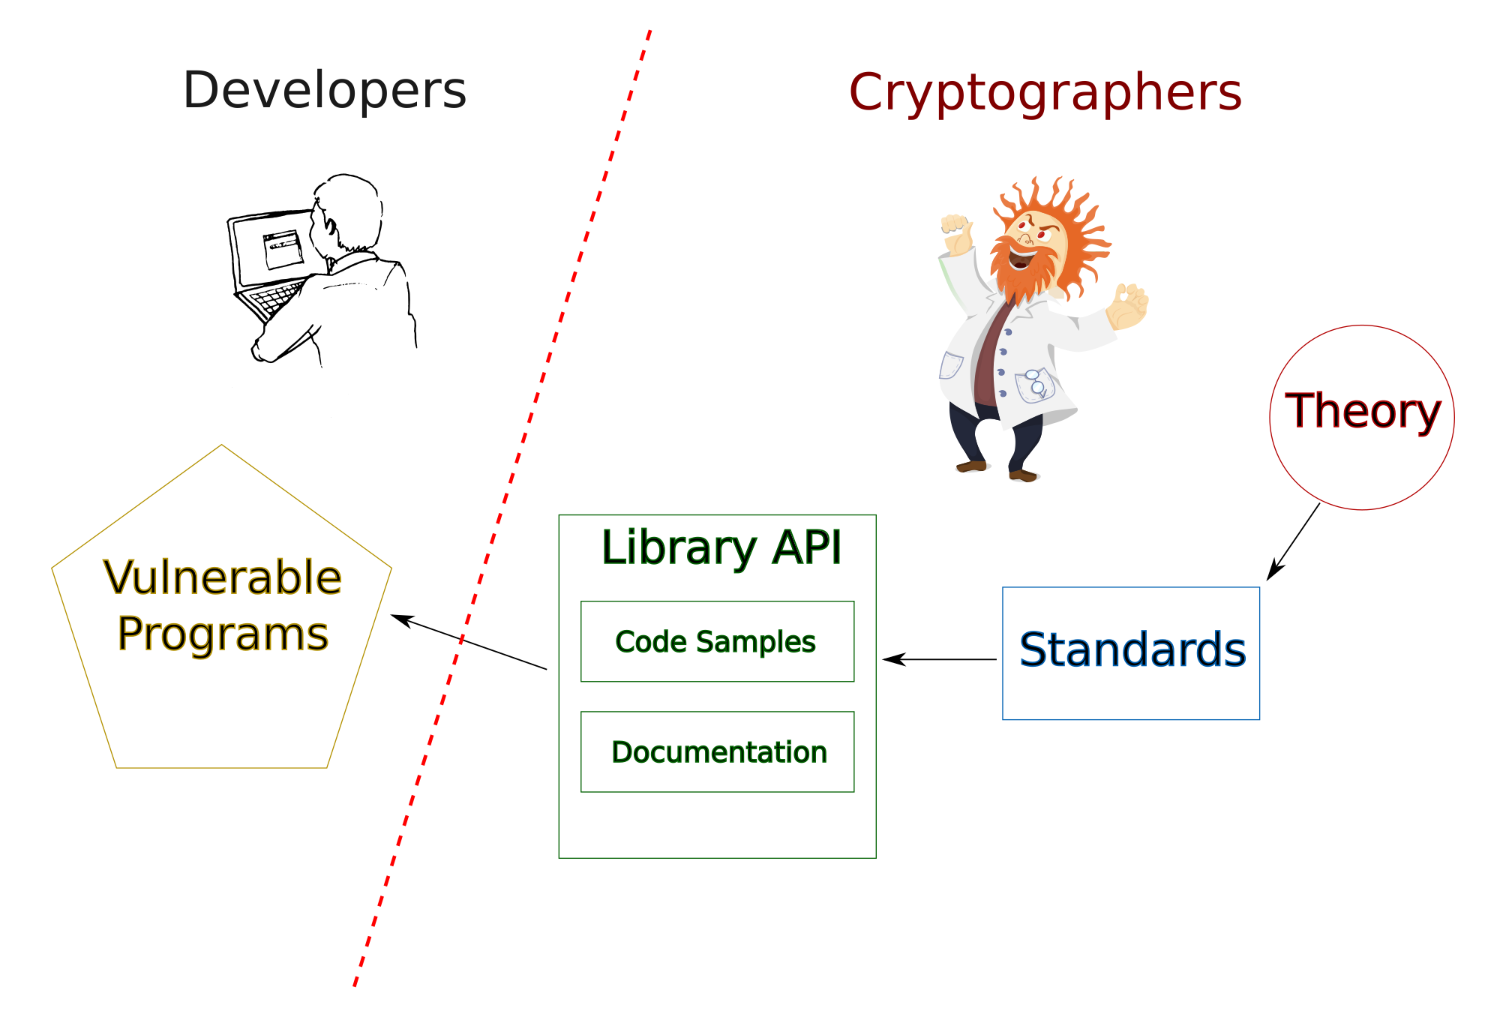
\includegraphics[width=0.8\textwidth]{text/media/developers_cryptographers.png}
    \caption[~Začlenění kryptografie do softwarového vývoje]{Začlenění kryptografie do softwarového vývoje podceňuje rozdíl mezi expertízou kryptografů a~vývojářů. Převzato z~\cite{das2014iv}.}
\end{figure}

\section{Kryptografická primitiva a kryptografické protokoly}

Než shrneme zjištění získaná literární rešerší problematiky bezpečného (resp.\ zranitelného) po\-u\-ži\-tí kryptografie v~kódu, při\-po\-me\-ne\-me pro čtenářovo pohodlí některé základní kryptografické algoritmy běžně používané v~dnešních aplikacích a~některé jejich důležité charakteristiky relevantní pro jejich bezpečné použití. Tyto kryptografické algoritmy lze zjednodušeně rozdělit na dvě kategorie: První kategorií jsou kryptografická primitiva, tedy jakési stavební kameny kryptografie, druhou jsou kryptografické protokoly, tj.~úplné specifikace zabezpečené komunikace.

\subsubsection*{Symetrická šifra a její autentizace}

Symetrická šifra je kryptografické primitivum sloužící k~utajení informace. Toho dosahuje šif\-ro\-va\-cí transformací, která pomocí tajného klíče převádí otevřený text (OT) na šifrový text (ŠT), a~k~ní inverzní de\-šif\-ro\-va\-cí transformací. Ta pro úspěšné dešifrování zprávy vyžaduje v~případě symetrické šifry použití téhož klíče, kterým byla zpráva zašifrována.

Základní vlastností, kterou od dnešních symetrických šifer očekáváme, je IND-CPA neboli \emph{nerozlišitelnost při útoku s~výběrem otevřeného textu} (angl.~\textit{indistinguishability under chosen-plaintext attack}):

\begin{definition}[IND-CPA]
    Vlastnost IND-CPA symetrické šifry je definována jako neschopnost pomyslného nepřítele uspět v~následující hře:

    Nepřítel libovolně zvolí dva OT, které jsou následně zašifrovány (stejným) neznámým klíčem. Dále má nepřítel k~dispozici šifrovací orákulum\footnote{Orákulum je v~informatice obecně termín pro stroj s~neznámou implementací, který se ale chová deterministicky, tj.~na daný vstup vždy odpoví stejným výstupem. Šifrovací orákulum tedy umožňuje nepříteli zašifrovat libovolný otevřený text bez prozrazení tajného klíče.} (ale ne samotný klíč). Pokud nepřítel ani v~takové situaci prokazatelně nedokáže s~významnou pravděpodobností rozeznat, který ŠT přísluší kterému OT, pak o~šifře řekneme, že je IND-CPA.~\cite{das2014iv}
\end{definition}

Dnes používané konstrukce symetrických šifer, které jsou schopné za určitých podmínek tuto vlastnost zaručit, rozdělujeme na šifry \emph{proudové} a~\emph{blokové}.

Proudové šifry z~klíče pevné velikosti deterministicky generují \emph{posloupnost hesla} (v~angličtině \textit{keystream}), která určuje transformace jednotlivých znaků při šifrování a~dešifrování zprávy. Aby šifra splnila vlastnost IND-CPA, je ale potřeba zajistit, že při opakovaném použití stejného šifrovacího klíče nedojde k~vygenerování totožné posloupnosti hesla a~tedy totožných substitucí. Za tímto účelem do vlastního šifrovacího a~dešifrovacího algoritmu vstupuje zpravidla kromě klíče a~OT/ŠT ještě \emph{inicializační vektor} (IV) --- nepředvídatelná jednorázová hodnota (\textit{number used once} neboli zkráceně \textit{nonce}), která zaručuje jedinečnost posloupností hesel napříč šifrováními. Inicializační vektor je veřejný parametr --- pro pozdější úspěšné dešifrování zprávy musí být adresátovi předán spolu s~šifrovým textem.

Blokové šifry na rozdíl od těch proudových negenerují nekonečnou posloupnost hesla; kryptoanalýze brání tak, že zprávu šifrují po blocích většího počtu znaků najednou (dnes nejčastěji 128 bitů, tj.\ 16 bajtů). Vzhledem k~tomu, že (de)šifrovací transformace bloku závisí pouze na klíči, pro dosažení IND-CPA nestačí zprávu jednoduše rozdělit na bloky příslušné velikosti a~každý blok zašifrovat zvlášť. Uvažme například blokovou šifru nad českou abecedou s~mezerou a~interpunkcí, velikost bloku 4~znaky a~otevřený text \texttt{ZDAR, NAZDAR}. Šifrování by proběhlo zvlášť nad bloky ``\texttt{ZDAR}'', ``\texttt{, NA}'' a~``\texttt{ZDAR}'' --- to znamená, že první a~poslední blok šifrového textu by byly shodné. Z~toho by útočník dokázal usoudit, že šifrovaná zpráva nemůže být žádná taková, kde první blok není shodný s~posledním, což by mu výrazně zlehčilo prolomení šifry.\footnote{Didakticky tento problém demonstruje fenomén ``ECB tučňáka'' popsaný například v~\cite{ecbpenguin}.}

Řešením tohoto problému (a~mnoha dalších, které by takové použití přinášelo) a~tedy dů\-le\-ži\-tým prostředkem pro bezpečné použití blokových šifer jsou \emph{operační módy} (někdy též \emph{provozní režimy}, angl.\ \textit{modes of operation}). Triviální operační mód, který každý blok OT zašifruje zvlášť toutéž transformací (a~tedy nesplňuje IND-CPA), se nazývá \textit{electronic codebook mode}, zkr.~ECB. Za bezpečné\footnote{Za určitých podmínek.} jsou považovány z~klasických operačních módů například \textit{cipher block chaining mode} (CBC), \textit{cipher feedback mode} (CFB) a~\textit{output feedback mode} (OFB), které z~podobného důvodu jako proudové šifry navíc vyžadují jako vstup inicializační vektor. Vedle klasických operačních módů navíc existují i~operační módy se zvláštním účelem, např.\ \textit{XEX-based tweaked-codebook mode with ciphertext stealing} (XTS) speciálně navržený pro šifrování disků nebo tzv.~autentizované módy \textit{Galois/counter mode} (GCM), \textit{counter with CBC-MAC} (CCM) a~mód EAX, jejichž význam popíšeme vzápětí.

Samotné šifrování ne\-do\-ká\-že komunikaci zcela zabezpečit: Zaprvé nezaručuje integritu a~autenticitu tajných zpráv, zadruhé je jeho použití možné pouze v~případě, že se již dříve obě strany domluvily na tajném klíči. První z~těchto problémů byl v~aplikované kryptografii tradičně řešen explicitním použitím MAC funkcí (\textit{message authentication code}), které na základě dat a~tajného klíče vypočtou kód pevné velikosti, který slouží jako důkaz pravosti a~nepoškozenosti zprávy. Určité vylepšení nad tímto postupem přinášejí \emph{autentizované šifry}, které kombinují použití symetrické šifry a~MAC do jednoho algoritmu, resp.\ do jedné abstrakce. Výstupem šifrování je kromě šifrového textu \emph{autentizační tag}, který musí být spolu s~ŠT předán dešifrovacímu algoritmu. Pokud útočník šifrový text za přenosu modifikuje, tag vypočtený při dešifrování se nebude shodovat s~tím přijatým a~dešifrování selže. Některé autentizované šifry navíc nabízejí autentizaci tzv.~\emph{asociovaných dat}, tedy části zprávy, která není šifrována.~\cite{Dworkin2007}

Mezi rozšířené symetrické šifry, které jsou dnes považovány za bezpečné, patří proudové šifry ChaCha20 a~Salsa20, bloková šifra AES (\textit{Advanced Encryption Standard}) a~na nich založená AEAD schémata\footnote{\textit{Authenticated Encryption with Associated Data}.} ChaCha20-Poly1305 a~AES v~jednom z~autentizovaných módů zmíněných výše (nejčastěji GCM). Z~již prolomených, ale historicky hojně používaných symetrických šifer stojí za zmínku především proudová šifra RC4 (Arcfour) a~bloková šifra DES (\textit{Data Encryption Standard}).

\subsubsection*{Asymetrická kryptografie}

V~předchozích odstavcích jsme popsali šifrovací systémy, které pro šifrování i~dešifrování používají shodný klíč. Takové schéma umožňuje utajit komunikaci dvou ``rovnocenných'' stran, ale nepokryje situace, kdy požadujeme například, aby jeden účastník komunikace mohl zprávu zašifrovat (podepsat) a~kdokoli jiný ji mohl posléze dešifrovat (podpis ověřit), aniž by ale mohl sám takový šifrový text (podpis) vytvořit. Další problém, který nám asymetrická kryptografie pomáhá vyřešit, je problém ustanovení klíče: Aby strany mohly vůbec utajit komunikaci po ne\-za\-bez\-pe\-če\-ném kanále, musí se nejdřív dohodnout na tajném a~ne\-před\-ví\-da\-tel\-ném společném klíči.

Jedním z~nejstarších, přesto dodnes používaným algoritmem pro asymetrické šifrování a~podepisování je RSA (Rivest-Shamir-Adleman) založený na modulárním mocnění v~konečném tělese. Jeho bezpečnost stojí na složitosti problému faktorizace modulu --- součinu dvou velmi velkých prvočísel, které zná pouze vlastník soukromého klíče. Dalším rozšířeným algoritmem pro digitální podepisování je \emph{Digital Signature Algorithm} (DSA) založený na (klasickém) problému diskrétního logaritmu\footnote{Tj.~nalezení logaritmu zadaného čísla při zadaném základu v~konečném tělese.} a~jeho modernější verze (ECDSA, EdDSA) využívající eliptické křivky.

Pro ustanovení společného klíče pro symetrické šifrování přes nezabezpečený kanál se používá zpravidla některá varianta algoritmu \emph{Diffie-Hellman}. Podobně jako u~DSA existují dvě varianty: Starší z~nich je založená na klasickém problému diskrétního logaritmu, v~současnosti preferovaná je varianta s~eliptickými křivkami (\textit{Elliptic Curve Diffie-Hellman}, ECDH)~\cite{haakegaard2015elliptic}.

\subsubsection*{Hašovací funkce a funkce pro odvození klíče}

Kryptografické hašovací funkce jsou jednosměrné bezkolizní funkce, které libovolně velkým datům přiřadí číslo pevné velikosti (případně velikosti, která je zadána jako vstupní parametr\footnote{Např.\ algoritmus BLAKE3 podporuje výstup libovolné velikosti.}). Jejich jednosměrnost spočívá v~tom, že ze znalosti obrazu (výstupu\footnote{Výstup kryptografické hašovací funkce se označuje jako \emph{hash}, případně \emph{fingerprint}, \emph{message digest} (MD) nebo \emph{manipulation detection code} (MDC).}) nelze efektivně (v~polynomiálním čase) vypočíst vzor (vstup); bezkoliznost znamená, že neexistuje efektivní algoritmus pro nalezení libovolných dvou vzorů se stejným obrazem (odolnost proti kolizi 1.~druhu) a~speciálně k~pevně zadanému vzoru nelze efektivně nalézt jiný vzor se stejným obrazem (kolize 2.~druhu). Hašovací funkce slouží jako důkazy o~integritě zpráv a~lze pomocí nich např.\ konstruovat MAC funkce (tzv.~\textit{hash-based} MAC neboli HMAC). Za určitých předpokladů mohou hašovací funkce sloužit také k~ověření znalosti nějaké informace bez toho, aby tato informace byla explicitně uchovávána (např.\ uživatelské heslo v~databázi).

Funkce pro odvození klíče (\textit{Key Derivation Function}, KDF) jsou podobné hašovacím funkcím v~tom smyslu, že na základě libovolně dlouhého vstupu (hesla) vyprodukují nepředvídatelný řetězec zadané délky. Jejich návrh ale zároveň zpravidla zahrnuje záměrně výpočetně náročnou operaci (např.\ iterovanou aplikaci hašovací funkce) za účelem zamezení útokům hrubou silou (\textit{brute-force attack}) a~náhodnou sůl (\textit{salt}) jako obranu proti slovníkovým útokům (\textit{dictionary attack} nebo přesněji \textit{rainbow table attack}).

Mezi dnes běžně používané kryptografické hašovací funkce patří především různé varianty algoritmu \emph{Secure Hashing Algoritm} (SHA) --- s~výjimkou SHA-1, pro který byla v~roce 2017 nalezena kolize 1.~druhu~\cite{shattered} --- a~dále např.\ algoritmy BLAKE, RIPEMD, bcrypt nebo Argon. Pro odvození klíče z~hesla se dnes standardně používá funkce PBKDF2 (\textit{Password-Based Key Derivation Function 2}), která kromě hesla a~soli jako vstupní parametry přijímá počet iterací, hešovací funkci a~požadovanou délku výstupu~\cite{rfc2898}. 

\subsubsection*{Generátory náhodných čísel}

Generování náhodných, resp.\ pseudonáhodných čísel (RNG, resp.\ PRNG) není samo o~sobě kryptografickou operací, bez\-peč\-nost mnoha kryptografických algoritmů se však právě od kvality zdroje náhodnosti odvíjí. Například od klíče pro symetrickou šifru očekáváme maximální entropii, jinými slovy chceme, aby útočníkovi pro prolomení šifry (i~se znalostí použitého generátoru) nezbylo nic lepšího, než vyzkoušet všechny binární řetězce příslušné délky. Konkrétně od \emph{kryptograficky bezpečných generátorů pseudonáhodných čísel} (CSPRNG) vyžadujeme dvě základní vlastnosti --- nepředvídatelnost dalšího bitu na základě jakékoli známé posloupnosti předchozích bitů (\textit{next-bit test}) a~nemožnost rekonstrukce předchozí hodnoty pseudonáhodné posloupnosti na základě zjištění vnitřního stavu (\textit{state compromise}).~\cite{csprng}

Výchozí pseudonáhodné generátory ve standardních knihovnách programovacích jazyků ale takovou kvalitu zpravidla neposkytují, neboť jejich účelem není bezpečnost, ale rychlost --- ve většině situací mimo kryptografii postačuje pouze \emph{zdánlivě nepředvídatelná} náhodnost.

\subsubsection*{Protokol TLS}

\textit{Transport Layer Security} (TLS) je kryptografický protokol, který ``\textit{umožňuje aplikacím s~architekturou klient–server komunikovat přes internet způsobem, který zabraňuje odposlechu, manipulaci a~falšování zpráv}''~\cite{tls13rfc}. K~tomu TLS využívá mimo jiné kryptografická primitiva popsaná výše.

Použití TLS obnáší především dvě specifika. Prvním z~nich je volba správné verze protokolu --- verze TLS 1.1 a~starší\footnote{Včetně protokolu SSL (\textit{Secure Sockets Layer}), který je předchůdcem TLS.} jsou ze své podstaty zranitelné vůči různým druhům útoků, které v~nejhorším případě dokážou šifrování (resp.\ autentizaci a~integritu) úplně prolomit~\cite{poodle}. V~dnešních aplikacích je proto nutné používat výhradně TLS verze 1.2 nebo 1.3.

Druhým specifikem použití protokolu TLS je autentizace serveru vůči klientovi, případně výjimečně i~klienta vůči serveru. Zahájení komunikace mezi klientem a~serverem probíhá v~TLS protokolu prostřednictvím \textit{TLS handshake}, v~jehož průběhu mimo jiné server pošle klientovi svůj certifikát, neboli doklad o~pravosti jeho veřejného klíče podepsaný \emph{certifikační autoritou}. Klient posléze musí tento certifikát validovat, aby se ujistil, že není falešný nebo neplatný. Zaprvé musí na základě sady kořenových certifikátů ověřit řetěz certifikace a~ověřit pravost certifikátu, dále musí validovat datum expirace certifikátu a~ověřit, že certifikát nebyl certifikační autoritou revokován. Validace certifikátu je stručně řečeno složitým --- a~jak uvidíme později, pro vývojáře aplikací problematickým~\cite{comparing2017} --- úkolem, přičemž její nesprávná implementace může v~nejhorším případě útočníkovi poskytnout příležitost pro velmi přímočarý útok typu \textit{man-in-the-middle}.

\section{Návrh kryptografických rozhraní}

Prvním významným aspektem bezpečnosti kryptografických knihoven je návrh jejího pro\-g\-ra\-má\-tor\-ského rozhraní. Autoři Green a~Smith v~článku~\cite{greensmith} z~roku 2016 poukazují na závažnost chyb, kterých se vývojáři dopouštějí při práci s~kryptografií, a~formulují 10 doporučení pro bezpečný návrh kryptografických rozhraní. Poznamenávají, že kryptografická rozhraní pro programování aplikací (\emph{Application Programming Interface}, API) jsou specifická především tím, že jejich špatné použití nevede k~tak viditelným chybám jako chybné použití ne-kryptografických API, a~proto je jejich zneužití mnohem hůře identifikovatelné. Zároveň připomínají, že vytváření snadno použitelných bezpečnostních mechanismů je lepším prostředkem pro zabránění vzniku chyb, než vzdělávání uživatelů, aby dokázali bezpečně pracovat se softwarem, který je složitý a~matoucí. Mezi svých 10 doporučení pro návrh kryptografických API zařazují především:

\begin{itemize}
    \item \textbf{Kryptografie má být zahrnuta do standardních API.} \enskip
        Autoři vychází ze skutečnosti, že vývojáři typicky nepřemýšlí v~kryptografických termínech --- svůj problém neformulují jako výměnu klíčů pomocí asymetrického kryptografického schématu, validaci certifikátu a~volbu blokové symetrické šifry, jejího operačního modu a~autentizačního mechanismu. Vývojáři chtějí typicky řešit problémy jako je navázání tajné komunikace s~dalším zařízením, stáhnutí a~ověření integrity souboru z~vzdáleného serveru, bezpečné uložení hesla do databáze, zašifrování souboru pomocí hesla, apod. Pokud je kryptografický protokol enkapsulovaný ve standardním API, např.\ API pro komunikaci pomocí HTTPS nebo SSH, pak je problém s~chybným použitím kryptografie koncovým vývojářem téměř zcela eliminován.

    \item \textbf{API musí být dostatečně flexibilní.} \enskip
        V~situaci, kdy API neumožňuje dostatečně flexibilní použití, aby pomocí něj vývojář dosáhl svého cíle, se může stát (a~podle zkušeností autorů se tak skutečně děje), že se bude vývojář pokoušet daný bezpečnostní mechanismus obcházet nebo ho nějakým způsobem ohýbat, což přirozeně zvyšuje riziko vzniku chyby.

    \item \textbf{API musí být srozumitelné i~pro ne-experty.} \enskip
        Kryptografie je složitá, ale její složitost lze v~mnoha případech před jejími uživateli skrýt. Pokud knihovna po uživateli například vyžaduje explicitně specifikovat operační mód, který má být použitý při šifrování algoritmem AES, zvyšuje se tím šance, že vývojář použije nebezpečný mód, např.\ ECB~\cite{comparing2017}. Podobně pokud bude knihovna po uživateli vyžadovat při šifrování hodnotu inicializačního vektoru, snadno se stane, že vývojář použije pokaždé stejnou konstantní nebo snadno predikovatelnou hodnotu a~tím nevědomě kompromituje kvalitu šifrování~\cite{das2014iv}.

        Autoři proto doporučují kryptografické detaily schovat do implementace a~uživateli z\-pří\-stup\-nit vysokoúrovňové API, které nebude vyžadovat detailní znalost kryptografie.

    \item \textbf{API musí být obtížné použít špatně.} \enskip
        Podle autorů by návrháři kryptografických API měli vyvinout co největší úsilí pro to, aby nesprávnému použití API úplně předcházeli; implementace by se zase měly za běhu snažit nesprávné použití detekovat a~případně vyvolat chybu/výjimku. Zdůrazňují, že chyby by měly být zřetelné, srozumitelné, a~nemělo by být možné je snadno obejít či vypnout (nebo by alespoň mechanismus umožňující chybu obejít měl být explicitně označen jako nebezpečný).

    \item \textbf{Výchozí parametry musí být bezpečné a~jednoznačné.} \enskip
        Většina uživatelů softwaru použije jeho výchozí konfiguraci~\cite{Daswani2007}, je tedy vysoce žádoucí, aby taková konfigurace nepoužívala slabé parametry, nebo v~nejhorším případě parametry, které naprosto anulují bez\-peč\-nost\-ní záruky daného kryptografického algoritmu.

        Jako odstrašující příklad lze použít knihovnu PyCrypto. Před tím, než byl v~roce 2013 její vývoj ukončen, dlouho plnila roli de facto standardní kryptografické knihovny pro jazyk Python~\cite{keckmasters}, byť z~hlediska kvality API trpěla vážnými nedostatky. Například její funkce pro vytvoření objektu pro šifrování algoritmem AES měla nepovinný parametr \texttt{IV} reprezentující inicializační vektor, o~kterém dokumentace knihovny píše, že pokud jej programátor nespecifikuje, tak se použije výchozí hodnota se samými nulami~\cite{pycryptodoc}. Stejně nebezpečný byl výchozí operační mód pro šifrování blokovými šiframi, kterým byl mód ECB~\cite{das2014iv}.

        S~podobným problém se potýkalo i~kryptografické rozhraní Java Cryptography Architecture (JCA), které po uživateli sice nevyžadovalo explicitně nastavit operační mód šifry, ale výchozí hodnota byla ponechána na implementaci, přičemž některé implementace jako výchozí hodnotu zvolily opět zranitelný mód ECB~\cite{greensmith}.

    \item \textbf{Knihovna by měla nabízet testovací mód.} \enskip
        Další doporučení vychází z~poznatku, že vývojáři často chtějí svůj kód testovat deterministicky a~bez dopadu na výkon a~složitost kódu, který mohou bezpečnostní mechanismy do programu vnést. To je může vést k~tomu, že pro účely testování bezpečnostní mechanismy úplně vypnou nebo použijí parametry, které kvalitní knihovna vyhodnotí jako zranitelné (např.\ statický IV nebo klíč). Takové požadavky podle autorů nejsou nesmyslné, protože náhodnost obecně ztěžuje testování kódu. U~konvenčních řešení však hrozí scénář, že vývojáři například zapomenou po testování bezpečnost opět posílit a~nedopatřením vydají software používající takto oslabenou testovací konfiguraci. Autoři proto navrhují do knihoven zavést zvláštní testovací mód, který bude možné např.\ svázat s~konkrétním identifikátorem stroje, na kterém se kód bude testovat.

        Autoři nicméně uvádí, že v~době publikace si nejsou vědomi žádné knihovny, která by takovou funkcionalitu nabízela.
\end{itemize}

Návrhem kryptografických API se zabývají i~další autoři. Konkrétně studie~\cite{comparing2017, comparative2023} se zabývají porovnáním knihoven, které se snaží použití kryptografie zjednodušit, s~tradičními kryptografickými knihovnami. Důležitým závěrem jejich výzkumu je pozorování, že samotná jednoduchost API použití knihovny nezjednodušuje, pokud knihovně chybí kvalitní dokumentace nebo nepokrývá dostatečně široké spektrum použití~\cite{comparing2017}.

Zajímavým pokusem o~pokrok v~bezpečnosti a~použitelnosti kryptografických API (při zachování jejich flexibility) představuje knihovna FluentCrypto popsaná v~článku~\cite{fluentcrypto} z~roku~2021. Samotná knihovna měla poskytovat alternativní rozhraní ke kryptografickému modulu runtimu Node.js, zajímavou ji ale činí především její přístup k~volbě kryptografických algoritmů a~jejich parametrů. Do procesu výběru kryptografických parametrů měli vstupovat tři aktéři: Prvním aktérem byli experti na kryptografii, kteří pomocí zvláštní syntaxe v~tzv.\ ``CryRule'' souborech popsali pravidla, resp.\ omezení, kterými se použití kryptografie muselo řídit (např.\ povolené šifry, operační módy, délky klíčů, atd.). Druhým aktérem byli aplikační vývojáři, kteří pouze použili rozhraní knihovny způsobem, který jim dával smysl. (Rozhraní knihovny bylo zároveň navrženo tak, aby bylo jeho intuitivní použití s~implicitními parametry bezpečné, ale přesto umožňovalo pokročilou konfiguraci.) Posledním aktérem byl samotný runtime knihovny, který za doby běhu kontroloval soulad volání API s~definovanými požadavky. Přestože v~experimentech porovnávajících FluentCrypto s~výchozím rozhraním pro kryptografii v~Node.js knihovna dosahovala pozoruhodných výsledků~\cite{fluentcrypto}, z~důvodů, které nám nejsou známé, bohužel projekt FluentCrypto již není aktivní (odkaz na repositář knihovny v~článku je nefunkční a~její kód nelze ani jinak dohledat). Přesto se nám jeho přístup k~návrhu kryptografických knihoven a~jejich rozhraní zdá být velmi slibný.

\section{Programovací jazyky}

Problematikou chyb v~použití kryptografie se dále zabývají autoři Das a~kol., kteří v~článku~\cite{das2014iv} z~roku~2014 z\-kou\-ma\-jí kryptografické knihovny ze 7~úhlů (opakované použití IV, výchozí hodnoty, zahlcení funkcemi, chybějící funkce, dokumentace, ukázkový kód a~programovací jazyk) a~formulují doporučení pro budoucí vývoj kryptografických knihoven. Na jejich výzkum navazují Luo a~kol.\ článkem~\cite{comparative2023} z~roku~2023, v~němž skrze řízený experiment porovnávají použitelnost rozhraní pro symetrickou kryptografii 9~růz\-ných kryptografických knihoven a~opět formulují doporučení pro bezpečně použitelné kryptografické knihovny. Obě zmíněné studie se mimo jiné dotýkají volby programovacího jazyka, ve kterém knihovna svoje rozhraní nabízí, a~zdůrazňují výhody \emph{paměťově bezpečných} a~\emph{silně typovaných} jazyků, resp.\ rozhraní.

\subsection{Paměťová bezpečnost}

Každý program potřebuje ke svému běhu určité množství paměti, do které si ukládá např.\ vstup od uživatele, mezivýsledky výpočtů pro pozdější zpracování, stav vykonávání programu, apod. Různé programovací jazyky přitom poskytují různé úrovně abstrakce nad prací se ``surovou'' pamětí prostřednictvím proměnných, struktur, polí, objektů, atd. Relevantní jsou pro nás tři aspekty paměťové bezpečnosti: dynamická alokace paměti, která může vést ke zranitelnostem typu \textit{use-after-free}, dále kontrola přístupu do paměti (\textit{bounds checking}), bez které je snadné do programu vnést zranitelnosti typu \textit{přetečení bufferu}, a~nakonec neinicializovaná paměť, která může především způsobit \textit{vyzrazení důvěrných informací}.

Nízkoúrovňové jazyky, konkrétně jazyky symbolických instrukcí (angl.\ \textit{assembly languages}) a~jazyk C (potažmo C++), poskytují pouze velmi základní abstrakce nad pamětí v~podobě proměnných a~jejich typů. Starost o~správnou (a~bezpečnou) práci s~pamětí je v~těchto jazycích zodpovědností jejich uživatele. Dynamické alokace a~dealokace paměti programátor v~těchto jazycích dosáhne explicitním voláním API standardní knihovny (případně operačního systému); správná inicializace proměnných a~kontrola toho, že program nepřistupuje na adresy mimo rozsah paměti alokované pro data programu, je také ponechána na programátorovi. Jazyk C (a~do určité míry C++) je díky svojí jednoduchosti bezkonkurenčně výkonný a~dodnes široce používaný mj.\ v~implementacích operačních systémů, v~softwaru pro vestavěné systémy, apod., jeho nevýhodou ale je, že explicitní práce s~pamětí je náchylná na chyby a~z~hlediska bezpečnosti tudíž velmi riziková~\cite{gaynor2020} --- dokonce se ukazuje, že v~kryptografických knihovnách napsaných v~jazyce C a~C++ převažují zranitelnosti způsobené chybnou prací s~pamětí nad chybami kteréhokoli jiného druhu a~konstituují přes 37~\% zranitelností v~těchto knihovnách~\cite{youreallyshouldnt}.

Jazyky, které bývají označovány jako vysokoúrovňové, složitost (dynamické) alokace paměti před uživatelem schovávají jedním z~mnoha možných způsobů. Programy v~jazycích, které jsou interpretované (např.\ Python, JavaScript nebo PHP), se z~principu nemusí alokací paměti vůbec zabývat, protože ji obsluhuje běhové prostředí jejich interpretu. Dalším způsobem, jak abstrahovat (de)alokaci paměti, je mechanismus zvaný \textit{garbage collection} (GC), který dealokaci již nepotřebných bloků paměti ponechává na běhovém prostředí, které si uchovává seznam alokovaných bloků paměti a~platných odkazů na ně. (Mezi jazyky využívající tento přístup patří třeba jazyky Java nebo Go.) Poslední paměťovou abstrakcí hodnou zmínky je koncept vlastnictví paměti (\textit{ownership}) a~mechanismus \textit{borrow checking}, jehož průkopníkem je programovací jazyk Rust. V~tomto modelu má každá alokovaná proměnná svou ``vlastnící'' funkci a~jazyk za doby překladu vynucuje sadu pravidel pro její ``vypůjčování''. Takový přístup kombinuje bezpečnost vysokoúrovňových jazyků s~výkonem nízkoúrovňových jazyků, jeho záruky ale nejsou stoprocentní\footnote{V~některých krajních případech překladač \texttt{rustc} nechá uživatele napsat kód, který s~pamětí pracuje špatně~\cite{cvers}.}.

Paměťově bezpečné jazyky jako Python, Java nebo (do určité míry) Rust zároveň uživateli nedovolí přistoupit k~nealokované paměti (např.\ před začátek nebo za konec pole), například tím, že při takovém pokusu vyvolají výjimku (Python, Java), paniku (Rust) nebo vrátí zvláštní hodnotu (\texttt{undefined} v~JavaScriptu). Podobnými mechanismy takové jazyky zabrání programu číst neinicializovanou paměť. Takovými opatřeními tyto jazyky zabraňují tomu, aby vývojář vlastní vinou do své aplikace vnesl paměťovou chybu (přetečení bufferu, use-after-free, apod.). Do aplikací se takové chyby mohou stále dostat skrze zranitelnosti v~běhovém prostředí jazyka, implementaci překladače nebo knihovně samotného jazyka, takové situace jsou ale podstatně vzácnější --- už jen proto, že programovacích jazyků je výrazně méně než jejich uživatelů.

\subsection{Slabé a silné typování}

Dalším aspektem programovacích jazyků, který může potenciálně mít vliv na bezpečné použití (nejen) kryptografických knihoven, je jeho typový systém, neboli způsob, kterým programovací jazyk zaručuje správnost datových typů proměnných.

\begin{lstlisting}[caption={[~Rozhraní funkce pro inicializaci šifry v~knihovně OpenSSL]~Rozhraní funkce pro inicializaci šifry v~knihovně OpenSSL \cite{openssl-evp-encryptinit}},label={lst:openssl-evp-encryptinit},float,language=C]
int EVP_EncryptInit_ex(EVP_CIPHER_CTX *ctx,
                       const EVP_CIPHER *type,
                       ENGINE *impl,
                       const unsigned char *key,
                       const unsigned char *iv);
\end{lstlisting}

\begin{lstlisting}[caption={[~Rozhraní funkce pro inicializaci šifry v~Java Cryptography Architecture]~Rozhraní funkce pro inicializaci šifry v~Java Cryptography Architecture \cite{jca-encryptinit}},label={lst:jca-encryptinit},float,language=Java]
public void init(int opmode, Key key, AlgorithmParameters params);
\end{lstlisting}

Luo a~kol.~\cite{comparative2023} tuto problematiku demonstrují na příkladu rozhraní pro inicializaci symetrických šifer. Výpis kódu~\ref{lst:openssl-evp-encryptinit} ukazuje hlavičku funkce pro inicializaci symetrické šifry v~knihovně OpenSSL, výpis~\ref{lst:jca-encryptinit} deklaraci analogické funkce v~specifikaci Java Cryptography Architecture. Zatímco v~JCA knihovna explicitně rozlišuje typy šifrovacího klíče a~parametrů odvíjejících se od použitého algoritmu (tj.~je \emph{silně typuje}), funkce knihovny OpenSSL z~hlediska typů vůbec nerozlišuje mezi klíčem a~inicializačním vektorem. ``Slabé'' typování parametrů zvyšuje riziko, že je uživatel nedopatřením obmění nebo alokuje nesprávné množství paměti; pokud je typem ukazatel na \texttt{unsigned char} (namísto dedikovaného typu reprezentující pole bajtů), může to v~některých uživatelích navíc vyvolat dojem, že vstupem má být textový řetězec~\cite{comparative2023}.

Tendence vývojářů používat silné typy je přirozenou výhodou objektově-orientovaného programování (OOP) typického pro jazyk Java, objektový návrh ale není nutnou podmínkou pro použití silných typů. Výpis kódu \ref{lst:c-strong-types} představuje jeden možný způsob, kterým by šly (s~nulovou penalizací z~hlediska výkonu programu) odlišit typy pro klíč a~IV i~v~jazyce C.

\begin{lstlisting}[caption={~Možná implementace silných typů pro klíč a~IV v~jazyce C},label={lst:c-strong-types},float,language=C]
#include <stdint.h>
#include <stdlib.h>

constexpr size_t KEY_LENGTH = /* ... */;
struct Key { const uint8_t bytes[KEY_LENGTH]; };

constexpr size_t IV_LENGTH = /* ... */;
struct IV { const uint8_t bytes[IV_LENGTH]; };
\end{lstlisting}

Takové ``silné typy'' nabízejí vedle rozlišení jednotlivých parametrů funkcí a~zaručení správ\-ných velikostí polí ale i~další výhody.  Například v~jazycích podporujících zapouzdření (tedy rozlišení ``soukromých'' a~``veřejných'' členů struktur) lze takto vynutit, aby klíče nebo nonce byly konstruovány specifickým způsobem. Zatímco struktury z~výpisu~\ref{lst:c-strong-types} v~jazyce C uživatel může instancovat přímo (výpis~\ref{lst:c-instantiation}), například v~jazyce Rust lze využít implicitně soukromých členů struktur a~uživatele tak donutit IV vytvořit jednou z~funkcí, které nabízí její implementace (výpisy~\ref{lst:rust-encapsulation} a~\ref{lst:rust-instantiation}).

\begin{lstlisting}[caption={~Přímá inicializace struktury IV v~jazyce C},label={lst:c-instantiation},float,language=C]
int main(void)
{
    struct IV iv = {{0}};
    
    // ...
}
\end{lstlisting}

\begin{lstlisting}[caption={~Možné zapouzdření IV v~jazyce Rust},label={lst:rust-encapsulation},float]
mod cipher {
    pub const IV_LENGTH: usize = /* ... */;

    pub struct IV { bytes: [u8; IV_LENGTH] }

    impl IV {
        pub fn new_random() -> Self
        {
            // ...
        }
    }
}
\end{lstlisting}

\begin{lstlisting}[caption={~Nemožnost přímé inicializace zapouzdřeného IV v~jazyce Rust},label={lst:rust-instantiation},float]
fn main()
{
    /* This will not compile - 'bytes' is a private field. */
    let iv = cipher::IV { bytes: [0_u8; cipher::IV_LENGTH] };

    /* OK */
    let iv = cipher::IV::new_random();

    // ...
}
\end{lstlisting}

Opomenout nesmíme ani \emph{dynamicky typované} jazyky, tedy jazyky, které informaci o~typu proměnných zpracovávají nikoli staticky za doby překladu, ale dynamicky za doby běhu. Takové jazyky (z~těch populárních např.\ Python nebo JavaScript) umožňují typy proměnných měnit v~průběhu vykonávání programu a~nelze je proto snadno staticky validovat. U~takových jazyků nemá dobrý smysl hovořit o~silném nebo slabém typování; v~případě kryptografických knihoven těchto jazyků je zkrátka zodpovědností implementace, aby správnost argumentů funkce zkontrolovala v~době její invokace.

\section{Zdroje informací}

Dalším aspektem použití kryptografických knihoven, který se ukazuje být kritickým pro jejich (ne)bez\-peč\-nost, jsou zdroje informací, ze kterých může jejich uživatel vyjít. Plasticky toto demonstrují experimentální výzkumy použitelnosti kryptografických API: Účastníci jednoho takového experimentu~\cite{rustcryptoapis} dle autorů při používání kryptografických knihoven mimo jiné často spoléhali na ukázky kódu dostupné v~dokumentaci knihovny nebo online a~takové ukázky kódu pak automaticky považovali za důvěryhodné. Podobný experiment~\cite{comparing2017} dovedl výzkumníky k~dalším zajímavým, ale nepřekvapivým závěrům --- knihovny, které v~dokumentaci nevysvětlily význam různých parametrů (např.~IV) a~požadavky na ně (náhodnost, jedinečnost), byly účastníky častěji použity chybně. V~neposlední řadě se ukazuje, že se vývojáři (nehledě na úroveň zkušenosti) spoléhají na neoficiální (a~z~podstaty nedůvěryhodné) zdroje, jako jsou online diskuzní fóra~\cite{worrisome, rustcryptoapis, hurdles}.

Lze navíc očekávat, že s~pokračujícím rozmachem velkých jazykových modelů (LLM) jako ChatGPT nebo GitHub Copilot se bude tento problém obzvláště prohlubovat. To ilustruje i~výsledek nedávného experimentu, v~němž si jistý bezpečnostní výzkumník registroval v~indexu PyPI\footnote{PyPI je index balíčků pro jazyk Python.} falešný balíček, jehož jméno si v~odpovědi na dotaz týkající se softwarového vývoje vymyslela umělá inteligence. Během následujících 3~měsíců nasbíral balíček podle jeho autora přes 15~000~stažení a~do svých projektů jej mělo přidat i~několik velkých společností, např.\ společnost Alibaba.~\cite{ai-hallucinate}

Literatura zároveň podrobně zkoumá konkrétní druhy nejasností, se kterými se uživatelé kryptografie potkávají. Jedna studie~\cite{dazedandconfused} provádí ruční analýzu 500 diskuzních vláken na populárním fóru Stack Overflow\footnote{\url{https://stackoverflow.com}}, které kategorizuje do 10 kategorií. Jako kritické se v~ní projevují kategorie otázek ohledně šifrování (např.\ operačních módů, zarovnání/výplně, šifrování pomocí hesla, kódování šifrového textu), certifikátů, interoperability různých knihoven, ale také třeba správy kryptografických klíčů. Další studie~\cite{hurdles} provádí statistickou analýzu (clustering) téměř 100~000 příspěvků na témže fóru a~ukazuje, že mezi největší překážky pro vývojáře v~implementaci kryptografických scénářů patří složitost API knihoven a~neznalost složitějších kryptografických konceptů (např.\ digitálních certifikátů, asymetrické kryptografie nebo hašování).

\section{Doporučení pro kryptografické knihovny}

Mnoho článků zmíněných v~předchozích odstavcích vedle výsledků empirického výzkumu poskytuje i~konkrétní doporučení pro kryptografické knihovny, které na závěr této kapitoly shrneme.

Prvním kritickým aspektem bezpečné použitelnosti knihoven je kvalita dokumentace, dostupnost bezpečných a~realistických ukázek kódu a~spolehlivost ostatních online zdrojů. Dokumentace nemá být pouhý seznam okomentovaných hlaviček funkcí, ale má vysvětlovat scénáře, ve kterých je jednotlivé algoritmy vhodné použít a~co musí jejich parametry splňovat~\cite{rustcryptoapis, comparing2017}. Zároveň musí upozornit uživatele na nevhodné konfigurace, např.\ zastaralé algoritmy. Dále je důležitý bezpečný návrh API, který ve výchozím bezpečném režimu umožní snadné použití knihovny běžnými vývojáři, ale zároveň poskytne i~explicitní konfiguraci parametrů pokročilými uživateli~\cite{fluentcrypto, comparing2017}. Knihovnám, které nabízejí API zaměřené na jednoduchou použitelnost, by neměly chybět důležité podpůrné nebo pokročilé funkce, protože to uživatele od knihovny odradí nebo jej donutí improvizovat; zároveň by u~případných vysokoúrovňových abstrakcí mělo být popsáno, které algoritmy a~parametry knihovna v~jejich implementaci používá~\cite{comparative2023}. V~neposlední řadě knihovna může některým kritickým chybám zamezit volbou programovacího jazyka použitém jednak pro svou vlastní implementaci, jednak pro vystavované API~\cite{comparative2023}.


%---------------------------------------------------------------%

\chapter{Analýza vybraných kryptografických knihoven}
% ==================================================== %
% Chapter: Analýza vybraných kryptografických knihoven %
% Status: Final                                        %
% ==================================================== %
\label{analyza}

Teoretická východiska popsaná v~předchozích kapitolách nám poskytují dobrou představu o~tom, které aspekty open-source softwaru a~konkrétně kryptografických knihoven mohou být re\-le\-vant\-ní pro jejich důvěryhodnost a~bezpečnou použitelnost; tyto poznatky nyní vztáhneme ke kon\-krét\-ním vybraným knihovnám. Dále v~této kapitole navrhneme a~porovnáme několik způsobů identifikace čas\-tých chyb v~jejich použití a~tyto způsoby opět demonstrujeme na vybraných knihovnách. Tím získáme potřebné informace pro formulaci výsledné metody hodnocení knihoven.

\section{Model hrozeb}

Aby mělo dobrý smysl mluvit o~bezpečnosti kryptografických knihoven, je nejdřív potřeba vymezit, co takový pojem vůbec obnáší, tedy určit model hrozeb, které mohou bezpečnost knihoven kompromitovat. Ve specifickém případě kryptografických open-source knihoven přicházejí v~úvahu následující hrozby:

\subsection{Zadní vrátka v knihovně}

Termín \emph{zadní vrátka} (angl.\ \emph{backdoor}) v~softwaru obecně označuje jakoukoli funkcionalitu, kterou autor softwaru záměrně vloží do jeho kódu za účelem pozdějšího obcházení jeho bezpečnostních mechanismů.

Klíčovou vlastností zadních vrátek je jejich nedetekovatelnost pro uživatele, resp.\ pro kohokoli s~výjimkou jejich autora. Není proto v~našich silách v~této práci popsat obecný způsob, jak by se kryptografická zadní vrátka dala odhalit, snad kromě velmi průhledných případů. Ve zbytku textu se proto budeme zabývat převážně hrozbami, které přicházejí skrze jiné aktéry, než jsou správci knihovny. Existence zadních vrátek v~knihovně je přesto skutečnou hrozbou, kterou je třeba pro úplnost alespoň zmínit, přičemž se jeví jako vhodné tuto hrozbu rozlišit na dvě kategorie.

\subsubsection{Zadní vrátka na úrovni kryptografických algoritmů}

Do první kategorie hrozeb spadají situace, kdy autor knihovny buďto poskytuje vlastní kryptografický algoritmus, který byl záměrně navržen tak, aby šel autorem prolomit (taková hrozba je ale spíš zanedbatelná, protože zadní vrátka mají za cíl být pokud možno nedetekovatelná a~obrana proti takové hrozbě je triviální), nebo implementuje standardní kryptografický algoritmus způsobem, který navenek vypadá neodlišitelně od bezpečné implementace, ale jeho vnitřní fungování je upraveno tak, aby dávalo autorovi možnost kryptografii nějakým způsobem kompromitovat.

Příkladem implementace standardního algoritmu, který se dá takto ``kleptograficky'' upravit, je generování klíčů pro asymetrický algoritmus RSA, kdy zlomyslný vývojář takové implementace může prvočísla místo náhodného generování konstruovat specifickým způsobem, který mu (a~pouze jemu) později dovolí triviálně jejich součin faktorizovat\footnote{Jedna taková konstrukce je popsaná v~\cite{crypto-backdoors}.}. Dalším kryptografickým primitivem, které lze poměrně snadno a~úspěšně zmanipulovat, je generátor pseudonáhodných čísel. Takové implementace nicméně často spoléhají na složité a~neefektivní konstrukce, takže se dá alespoň částečně očekávat, že v~populárním open-source projektu by byly brzo odhaleny.~\cite{crypto-backdoors}

\subsubsection{Zadní vrátka v kryptografických API}

Do druhé kategorie hrozeb spadají situace, kdy autor knihovny korektně implementuje veřejně publikovaný a~odborníky přijímaný kryptografický standard (nebo takovou open-source implementaci využije jakožto závislost), ale v~některých konkrétních situacích záměrně použije slabé parametry nebo algoritmy a~tím kompromituje bezpečnost aplikací, které na jeho knihovně závisejí. V~takové situaci může ale být obtížné rozeznat, jestli autor takovou slabinu do kódu přidal úmyslně, nebo byla zapříčiněna jeho neznalostí nebo nedbalostí. Z~tohoto důvodu se domníváme, že nemá příliš dobrý smysl rozlišovat mezi úmyslnou sabotáží knihovny a~vnesením zranitelného kódu z~nedbalosti, a~budeme proto v~tomto textu oba případy považovat za tutéž hrozbu, kterou popíšeme v~sekci~\ref{zranitelna-impl}.

\subsubsection{Obrany proti zadním vrátkům}

Klíčovými žádoucími vlastnostmi zadních vrátek jsou jejich nedetekovatelnost a~popiratelnost\footnote{Pro jejich autora je žádoucí, aby se při případném nařčení mohl odvolat na to, že něco přehlédl nebo udělal chybu.}, což činí jejich identifikaci značně problematickou. Pokud se vývojáři softwaru obávají možnosti, že použijí takto zmanipulovanou implementaci, mají přesto několik možností.

Jednou z~nich je použít knihovnu, která je dostatečně široce používaná a~kterou zároveň používají kredibilní organizace. Nevýhodou takového přístupu je, že nemusí vždy být zcela zřejmé, které organizace jsou kredibilní; např.\ jinak dosti pozitivně přijímaný americký Národní institut standardů a~technologie (National Institute of Standards and Technology, NIST) měl podle tajných dokumentů uniklých v~roce~2013 do pseudonáhodného generátoru Dual Elliptic Curve Deterministic Random Bit Generator (DUAL\_EC\_DRBG) takový backdoor umístit~\cite{crypto-backdoors}.

Další možností je v~aplikaci použít dvě různé implementace a~jejich výstupy zkombinovat, to znamená např.\ použít dva různé generátory pseudonáhodných posloupností a~jejich výstupy kombinovat operací XOR~\cite{crypto-backdoors}. V~případě šifrování přichází v~úvahu otevřený text zašifrovat sériově dvakrát (tj.~dvěma různými implementacemi, s~dvěma různými zdroji náhodnosti klíče, případně i~dvěma odlišnými šiframi)~\cite{snowden2019permanent}. Takový přístup se spoléhá na to, že pravděpodobnost existence zadních vrátek vytvořených jedním aktérem ve dvou různých šifrách, CSPRNG, atd., nebo jejich implementacích, je extrémně malá.

\subsection{Zranitelná implementace knihovny}
\label{zranitelna-impl}

Další hrozbu pro bezpečnost knihovny, potažmo aplikací, které na ní závisí, představuje přijetí zranitelného kódu (ať už úmyslně, nebo z~nedbalosti). I~správci projektů, kteří nemají žádné zlé úmysly, mohou vystavit uživatele knihovny nebezpečí, pakliže nebudou dostatečně důsledně řídit proces přispívání do kódu a~udržovat jeho kvalitu a~tím dovolí zlomyslným aktérům (nebo nedostatečně kompetentním vývojářům) přidat do knihovny zranitelný nebo nekvalitní kód.

\subsection{Zranitelné použití knihovny uživatelem}

Jak jsme již nastínili v~předchozí kapitole, i~implementace kryptografie, které jsou samy o~sobě bezpečné, jsou často aplikačními vývojáři používány nebezpečným způsobem. Při posuzování bez\-peč\-nos\-ti knihoven je proto potřeba uvažovat i~aspekt použitelnosti, tedy hrozbu, že vývojáři knihovny například špatným návrhem rozhraní, nevhodnou volbou výchozích hodnot a/nebo dokumentací knihovny uživatele nepřímo navedou k~tomu, že kryptografii použijí špatně a~vnesou tím do svého programu zranitelnost.

\section{Přehled zkoumaných knihoven}

Před samotnou analýzou stručně představíme knihovny vybrané pro bližší zkoumání. Při výběru knihoven byly zohledněny různé oblasti našeho zájmu, zejména různé programovací jazyky (nízká a~vysoká úroveň abstrakce jazyka, slabé a~silné typování) a~různé přístupy k~návrhu rozhraní knihovny.

\subsection*{OpenSSL}

OpenSSL, jedna z~nejstarších a~pravděpodobně i~historicky nejpoužívanějších kryptografických knihoven, byla vybrána především jako výchozí bod pro porovnání s~ostatními knihovnami. Je napsaná v~programovacím jazyce C a~vyvíjená už od roku~1998. Po více než čtvrtstoletí své existence nasbírala přes 250 různých CVE --- zdaleka nejvíc ze všech open-source kryptografických knihoven~\cite{nist-nvd}.

\subsection*{libgcrypt}

Knihovna libgcrypt je součástí projektu GNU Privacy Guard (GnuPG), populární open-source implementace specifikace OpenPGP. Knihovna poskytuje implementace nízkoúrovňových kryptografických algoritmů napsané v~jazyce C. Je široce používaná mimo jiné v~linuxovém ekosystému: Na standardní distribuci Ubuntu 23.10 na ní závisí až 192 balíčků, mezi nimi např.\ systemd, gnome-keyring nebo openvpn\footnote{Zjištěno příkazem \texttt{apt-cache rdepends libgcrypt20}.}.

\subsection*{rustls}

Knihovna rustls implementuje protokol TLS, resp.\ jeho bezpečné verze TLS~1.2 a~TLS~1.3, a~dává si za cíl být moderní alternativou k~OpenSSL. Kód knihovny je napsaný v~paměťově bezpečném jazyce Rust a~knihovna zároveň skrze \emph{foreign function interface} (FFI) poskytuje API kompatibilní s~jazykem C. Její první verze byla vydána v~roce~2016, i~přes své ``mládí'' je dnes ale používána mnoha projekty a~organizacemi. Registr Rust balíčků \url{https://crates.io} eviduje 712 balíčků závisejících na rustls, mezi nimi de~facto standardní Rust balíčky implementující HTTP klienty (reqwest), HTTP servery (hyper) nebo DNS (trust-dns-proto) čítající desítky milionů stažení\footnote{Viděno 2024-03-30.}.

\subsection*{ring}

Knihovna ring implementuje primitivní kryptografické algoritmy v~kombinaci jazyků Rust (25~\% kódu), C (30~\% kódu) a~assembler (39~\% kódu). Její kryptografický kód vychází z~knihovny BoringSSL\footnote{BoringSSL je open-source kryptografická knihovna založená na kódu z~OpenSSL, kterou pro své vlastní potřeby vyvíjí společnost Google.} a~jejím cílem je poskytovat Rust API, které bude ``\textit{jednoduché použít správně a~složité použít špatně}''~\cite{ringgithub}. V~ekosystému jazyka Rust jde o~de~facto standardní kryptografickou knihovnu, lze ji však použít i~z~jiných jazyků prostřednictvím FFI rozhraní. První veřejná verze knihovny byla vydána v~roce 2016. Od roku 2023 ke knihovně ring existuje FIPS-certifikovaná\footnote{FIPS~140-2 a~FIPS~140-3 jsou certifikace kryptografických algoritmů od amerického NISTu, které mimo jiné umožňují kryptografickým implementacím být použity v~systémech spadajících pod správu federální vlády USA.} alternativa implementující stejné rozhraní, totiž knihovna aws-lc-rs od společnosti Amazon Web Services.

\subsection*{cryptography.io}

Knihovna cryptography si dává za cíl být standardní kryptografickou knihovnou pro jazyk Python~\cite{pycagithub}. Poskytuje vysokoúrovňové API pro symetrické autentizované šifrování (modul ``Fernet'') a~validaci X.509 certifikátů, zároveň však dává uživateli přístup i~k~nízkoúrovňovým kryptografickým primitivům prostřednictvím modulu ``hazmat'' (\textit{hazardous materials}). Knihovna neimplementuje protokol TLS --- nejspíš proto, že v~jazyce Python je zahrnutý do standardní knihovny~\cite{pythontls}. Je napsaná v~Pythonu (76~\% kódu) a~Rustu (24~\% kódu), závisí na OpenSSL a~vystavuje API v~jazyce Python a~C. Její první verze byla vydána v~roce 2015.

\subsection*{PyCryptodome}

PyCryptodome je oproti ``cryptography'' o~něco starší kryptografická knihovna pro jazyk Python. Vznikla v~roce~2014 jako náhrada za neudržovanou a~zranitelnou knihovnu PyCrypto, která byla zároveň proslulá svým špatným návrhem, nedostatečnou podporou pro moderní algoritmy a~nebezpečnými výchozími hodnotami~\cite{comparing2017}. Cílem bylo poskytnout stávajícím uživatelům PyCrypto jednoduchý způsob, jak přejít na bezpečnější kryptografickou implementaci, a~je proto navzdory svému relativnímu ``mládí'' poměrně hodně svázaná zpětnou kompatibilitou. Autor projekt popisuje jako ``\textit{soběstačnou knihovnu nízkoúrovňových primitiv}''~\cite{pycryptodome}, její implementace je psaná v~Pythonu (55~\%) a~C (45~\%).

\section{Organizačně-technické procesy a kvalita kódu}

První z~oblastí našeho zájmu při zkoumání knihoven je organizace jejich vývoje, tedy především otázka toho, kdo knihovnu spravuje a~financuje, komu je dovoleno přispívat do kódu, jakým způsobem je nový kód revidován nebo jak projekt reaguje na bezpečnostní incidenty. S~tím úzce souvisí i~pokyny pro přispívání a~návody na formátování kódu.

Jednotlivé knihovny se značně liší mírou sdílnosti ohledně zmíněných procesů. Zatímco Open\-SSL na svých webových stránkách~\cite{openssl-web} detailně popisuje svoje organizační struktury (včetně seznamu jejich členů), požadavky na přispěvatele, pokyny pro nahlašování nalezených zranitelností a~politiky týkající se reakce na ně, o~autorovi/správci knihovny PyCryptodome oproti tomu nevíme téměř nic a~o~autorech cryptography.io a~ring jen velmi málo.

\subsection{Postup a použité nástroje}

Při rešerši dostupných informací lze vyjít především z~oficiálních zdrojů dané knihovny, tj.~we\-bo\-vých stránek, repositáře s~kódem, dokumentace, mailing listů, apod. Máme-li štěstí, dočteme se v~těchto zdrojích o~krocích, které projekt činí k~zabezpečení procesu vývoje a~zamezení vzniku zranitelností. V~některých případech ale informace zcela chybí nebo jsou neúplné.

Chceme-li si v~takovém případě udělat představu alespoň o~počtu vývojářů a~míře, ve které do kódu přispívají, můžeme se pokusit data vytěžit z~verzovacího systému. V~případě knihoven zkoumaných v~této práci je takový postup docela dobře proveditelný díky tomu, že repositáře s~jejich kódem jsou umístěné (nebo alespoň zrcadlené) na platformě GitHub, která pro získávání informací o~příspěvcích do kódu poskytuje webové API. Za tímto účelem byl během tohoto výzkumu vytvořen primitivní skript, který taková data o~příspěvcích umožňuje z~repositářů těžit. Jeho kód je k~dispozici na přiloženém médiu v~adresáři \texttt{appendices/commitfetch}.

Metriky popisující složitost kódu, jako je třeba průměrný počet řádků na soubor, maximální stupeň zanoření kódu, apod., mají tu výhodu, že se díky svému kvantitativnímu charakteru dají snadno automaticky měřit\footnote{V~případě jazyka C například nástrojem \texttt{cqmetrics}.}. Nevýhoda takového přístupu ale spočívá v~tom, že neexistují žádné univerzálně přijímané hranice pro bezpečné, resp.\ nebezpečné hodnoty jednotlivých metrik. Software, který tyto metriky počítá, navíc nemusí brát v~potaz různá specifika projektu, dokumentační komentáře nebo soubory, které obsahují pouze deklarace a~ne samotnou implementaci funkcí. V~neposlední řadě tyto metriky nezachytí důležité kvalitativní aspekty kódu, jako je jeho srozumitelnost, použití vhodných identifikátorů, apod. Z~těchto důvodů se nám nejeví jako dostatečně přínosné takový přístup použít. Kvalitu kódu lze kromě povrchové manuální revize kódu odhadnout třeba na základě přítomnosti (a~použitých technik) testů nebo začlenění průběžné integrace (\textit{continuous integration}, CI) do vývoje projektu.

\subsection{Výsledky}

\subsubsection*{OpenSSL}

Knihovnu OpenSSL zaštiťuje organizace OpenSSL Software Foundation. Vývoj projektu řídí dvě komise: První z~nich, Open\-SSL Management Committee (OMC), určuje vy\-so\-ko\-ú\-rov\-ňo\-vé směřování projektu a~rozhoduje o~ma\-na\-žer\-ských otázkách; Open\-SSL Technical Committee (OTC) má hlavní slovo v~technických zá\-le\-ži\-tos\-tech (včetně přispívání do kódu)~\cite{openssl-bylaws}. Z~hlediska financování se OpenSSL spoléhá na dary od sponzorů a~příjmy z~poskytování tzv.~\textit{support contracts} neboli komerční podpory na míru zákazníkům~\cite{openssl-donations}.

Klíčový institut, který OpenSSL používá, je \textit{committer} (přispěvatel). Tímto termínem projekt OpenSSL označuje status vývojáře, který může provádět netriviální změny v~kódu\footnote{Triviální změny jsou např.\ opravy gramatických nebo typografických chyb, jednořádkové opravy chyb nebo změny ve formátování (\emph{whitespace changes}). Na triviálnosti změny se musí shodnout autor se všemi, kdo změnu revidují.~\cite{openssl-committerpolicy}} a~schvalovat úpravy ostatních přispěvatelů. Status přispěvatele lze získat od OMC zpravidla na doporučení OTC a~může být kdykoli revokován na základě hlasování~\cite{openssl-committerpolicy}. Přispěvatelé jsou vázáni smlouvou \textit{Contributor License Agreement} (CLA), kolektivně zodpovídají za udržování kódu a~je od nich požadována pravidelná aktivita v~podobě autorství nebo revize alespoň 1~příspěvku (\textit{commitu}) za 2~čtvrtletí. V~současnosti má tento status 18~vývojářů~\cite{openssl-committerlist}.

Oficiální zdroje knihovny~\cite{openssl-committerpolicy} popisují taktéž proces revize a~schvalování změn v~kódu: Změny v~kódu musí být revidovány a~schváleny alespoň dvěma přispěvateli; alespoň jeden z~nich musí být členem OTC a~ani jeden z~recenzentů (\textit{reviewers}) nesmí být autorem kódu. Webová stránka dále poskytuje návod pro nahlášení zranitelností, popisuje bezpečnostní nedostatky knihovny a~deklaruje způsob, kterým jsou objevené zranitelnosti opravovány a~aplikovány záplaty. Vývoj knihovny je organizován prostřednictvím platformy GitHub.

Knihovna OpenSSL je napsaná v~jazyce C, který je proslulý svou náchylností k~bezpečnostně kritickým chybám. Projekt využívá funkce CI platformy GitHub a~s~každou změnou kódu spouští automatickou sadu testů, přičemž zároveň měří pokrytí kódu, které se v~době vzniku této práce pohybuje na úrovni 67~\%~\cite{openssl-codecov}, a~je též fuzzován prostřednictvím projektu OSS Fuzz~\cite{openssl-fuzz}. Knihovna splňuje certifikaci FIPS~140-2~\cite{openssl-fips} a~vlastní odznak OpenSSF Best Practices~\cite{openssl-openssf}, z~čehož můžeme soudit, že její vývoj probíhá bezpečným způsobem a~certifikované algoritmy jsou implementovány správně. Bohužel nám to ale nic neříká o~tom, jestli je knihovna pro uživatele srozumitelná nebo jestli je navádí k~bezpečnému použití.

\subsubsection*{libgcrypt}

Knihovna libgcrypt spadá pod organizaci projektu GnuPG. Ten spravuje skupina pěti správců uvedených na webové stránce projektu~\cite{gnupg-people}, někteří z~nich jsou navíc zaměstnanci společnosti g10\textsuperscript{code} a~vývoji se věnují na plný úvazek. Finance projekt GnuPG od roku 2022 čerpá (podobně jako OpenSSL) z~prodeje komerční podpory k~produktu GnuPG VS-Desktop, dříve byl financován sponzorskými dary~\cite{gnupg-new-future}.

Vývoj knihovny na rozdíl od OpenSSL neprobíhá na dedikované platformě, ale pro\-střed\-nic\-t\-vím veřejného \textit{mailing listu} (tj.~hromadné e-mailové komunikace). Samotný repositář s~kódem je přístupný skrz webovou stránku projektu. Projekt nijak nepopisuje požadavky na přispěvatele do kódu --- kdokoli může požádat o~to, aby byl do mailing listu přidán, navrhované změny v~kódu jsou revidovány nejspíš\footnote{Knihovna libgcrypt na rozdíl od OpenSSL nepopisuje proces, kterým je kód revidován. Informace, které podáváme v~tomto textu, jsou založené na nesystematické analýze archivů zpráv z~mailing listu.} na individuální bázi na základě obsahu spíš než autorství.

Projekt GnuPG splňuje požadavky OpenSSF Best Practices~\cite{gnupg-openssf} a~knihovna libgcrypt nabízí mód kompatibilní s~certifikací FIPS~140-3. Z~tohoto hlediska tedy můžeme knihovny libgcrypt a~OpenSSL prohlásit za srovnatelné, hlavní rozdíl mezi jejich organizací spočívá v~dostupnosti informací o~procesech souvisejících s~revizí a~přijímáním nového kódu.

Pozoruhodným faktem je, že navzdory podobnému stáří obou ``céčkových'' knihoven má lib\-g\-crypt v~databázi CVE pouze 15 záznamů, zatímco OpenSSL jich má 257. To může souviset se skutečností, že OpenSSL je co do počtů řádků kódu zhruba 4krát větší než libgcrypt~\cite{cloc-openssl-libgcrypt} a~na rozdíl od libgcrypt implementuje i~protokol SSL/TLS, definitivně rozhodnout o~skutečných příčinách tohoto rozdílu ale navzdory vší snaze nedokážeme --- potenciálních vysvětlujících proměnných je zkrátka příliš mnoho.

\subsubsection*{rustls}

Knihovna rustls je vyvíjená na platformě GitHub~\cite{rustls-gh}, kde jsou zároveň uvedeny všechny informace ohledně její organizace, struktury a~financování. Na rozdíl od předchozích dvou knihoven není rustls registrovaná v~projektu OpenSSF Best Practices a~tento odznak proto nevlastní; z~dostupných informací nicméně vyplývá, že kritéria pro jeho získání vesměs splňuje\footnote{V~průběhu psaní tohoto textu jsme se proto rozhodli správcům adopci odznaku navrhnout. Návrh je veřejný a~přístupný skrze URL \url{https://github.com/rustls/rustls/issues/1901} [cit. 2024-04-17].}.

Projekt je spravován projektovým manažerem a~trojicí vývojářů, dva z~nichž jsou full-time zaměstnanci iniciativy Prossimo, která je součástí neziskové organizace Internet Security Research Group a~usiluje o~``\textit{přechod internetové infrastruktury kritické pro bezpečnost na paměťově bezpečné implementace}''~\cite{prossimo}. Způsob vyvíjení kódu je do velké míry určen používanými nástroji --- diskuze nad změnami v~kódu, návrhy na nové funkce, apod.\ probíhají na GitHubu, stejně jako nahlašování zranitelností, které GitHub podporuje formou tzv.~\textit{security advisories}. Přestože od svého vzniku rustls čítá pouze 1~CVE\footnote{CVE-2019-15541.}, popisuje detailně politiky pro reakce na nahlášené zranitelnosti: Kromě samotné opravy, která je navíc zpětně aplikována na verze ne starší než 2~roky, mají být připraveny regresní testy a~zranitelnost nahlášena do databáze RustSec Advisory Database\footnote{RustSec Advisory Database~\cite{rustsec} je databáze zranitelností pokrývající všechny balíčky publikované pro\-střed\-nic\-tvím služby \url{https://crates.io}. Databáze je spravována oficiální pracovní skupinou jazyka Rust pro bezpečnost kódu (Rust Secure Code WG) a~je integrována přímo do standardního nástroje \textit{cargo}.}.

Knihovna rustls neklade žádné konkrétní požadavky na autory nových příspěvků kódu, podle dostupných informací může změnu navrhnout kdokoli. ``Readme'' projektu doporučuje nejprve vytvořit \textit{issue} a~chystanou změnu zkonzultovat se správci projektu; dále obsahuje pokyny ohledně velikosti jednotlivých změn (\textit{commitů}), praktik při psaní kódu, nutnosti testů, atd. Poslední slovo v~otázkách přijímání nového kódu mají správci projektu, přičemž na úrovni GitHub repositáře je vyžadována před schválením nového kódu (tzv.~\textit{pull requestu}, zkr.~PR) revize od alepoň jednoho člena s~rolí \textit{reviewer}.~\cite{rustls-gh}

\subsubsection*{ring}

Knihovna ring je z~hlediska organizace poměrně netypická --- nespravuje ji totiž tým vývojářů, jako v~případě rustls, ani obchodní nebo nezisková společnost, jako v~případě OpenSSL a~libgcrypt. Vlastníkem GitHub repositáře, jediným správcem knihovny a~zároveň nejaktivnějším vývojářem (z~hlediska počtu commitů za rok 2023) je uživatel Brian Smith~\cite{ringgithub}. Na svém profilu na platformě GitHub odkazuje na svůj blog, na kterém od roku 2015\footnote{Zjištěno pomocí Wayback Machine, \url{https://web.archive.org/web/20240000000000*/briansmith.org} [cit. 2024-04-16].} píše o~různých kryptografických tématech; na blogu i~na GitHub profilu ale chybí jakékoli informace o~samotném autorovi, jeho afilaci, kompetencích, apod.

Použitím technik \textit{open-source intelligence} (OSINT) se nám podařilo zjistit, že tento Brian Smith byl alespoň v~období cca~2010--2014 zaměstnancem společnosti Mozilla. Tomu nasvědčuje pracovní e-mailová adresa v~dřívější verzi blogu~\cite{briansmith-email} a~ticket v~systému Bugzilla~\cite{briansmith-bugzilla} z~roku 2010, ve kterém B.~Smith s~touto e-mailovou adresou úspěšně žádá o~přístup pro zaměstnance. V~souladu s~tímto zjištěním je i~archivovaný repositář na jeho GitHub profilu, který má obsahovat kód pro validaci certifikátů X.509 z~prohlížeče Mozilla Firefox~\cite{briansmith-firefox}, nebo také komentář stejnojmenného uživatele na sociální síti Reddit, který tvrdí, že pracuje na implementaci protokolu SSL v~prohlížeči Mozilla Firefox~\cite{briansmith-ssl}. Otázkou ale stále zůstává, jakou motivaci pro vývoj knihovny ring má její autor v~současnosti a~proč o~organizaci projektu poskytuje tak málo informací.

Ani ohledně procesů přispívání a~revize kódu není autor knihovny příliš sdílný. Historie repositáře ukazuje, že často změny v~kódu navrhuje i~schvaluje sám autor. V~``readme'' projektu je zmíněno, že je do projektu možné přispívat skrze PR, kromě požadavků na kompatibilní licenci však nejsou formulovány žádné konkrétní pokyny, požadavky na kód, apod. Za rok 2023 do kódu knihovny přispělo celkem 52~autorů, 33~z~nich pouze jedním příspěvkem; přes 90~\% všech příspěvků pocházelo od B.~Smitha a~autorů knihovny BoringSSL, ze které ring pravidelně slévá kód.

Projekt ring podle oficiálních záznamů OpenSSF splňuje požadavky odznaku Best Practices kvůli údajné chybějící statické a~dynamické analýze pouze na 82~\%, tento záznam byl ale vytvořen v~roce~2016 a~od té doby nebyl aktualizován.

\subsubsection*{cryptography.io}

Knihovna cryptography je vyvíjena skupinou Python Cryptography Authority (PyCA) na platformě GitHub. Navzdory názvu této skupiny nejde o~právnickou osobu se smluvním vztahem k~Python Software Foundation, ale jednoduše o~skupinu aktivních vývojářů z~open-source komunity. Jeden z~členů skupinu charakterizuje takto:

\blockquote{``\textit{Speaking as one of the members of the PyCA, no, there is no official licensing body and we are not licensed. [...] The Python Cryptographic Authority aspires to be the primary resource for Python developers needing cryptographic libraries, but our authority is derived solely from developer opinion of the quality of our software.}''~\cite{pyca-so}}

Není ale zřejmé, jaké jsou nároky na členství v~této skupině nebo jakým způsobem je knihovna cryptography (a~další, např.\ pyopenssl, pynacl nebo bcrypt) skupinou PyCA spravována. Webová stránka knihovny~\cite{pyca-web} zmiňuje pouze mailing list, IRC chat a~odkaz na GitHub repozitář, profil PyCA na GitHubu obsahuje pouze seznam členů a~odkazy na jednotlivé repositáře.

Oficiální stránky knihovny na druhou stranu popisují ``přísnou politiku'' pro přijímání kódu kvůli ``devastujícím následkům'' nesprávné implementace kryptografie. Kód nesmí do projektu přijmout nikdo z~jeho autorů, nové příspěvky do kódu musí doprovázet testy se 100\% pokrytím přidávaného kódu a~všechny testy musí procházet na 100~\%. Dokumentace knihovny zároveň obsahuje zvláštní sekci věnovanou bezpečnosti. Kanálem pro nahlašování zranitelností jsou podobně jako u~předchozích knihoven GitHub security advisories. Za zmínku stojí poměrně široká definice bezpečnostního problému, kterým se cryptography zavazuje zabývat:

\blockquote{``\textit{What is a~security issue? Anytime it’s possible to write code using cryptography’s public API which does not provide the guarantees that a~reasonable developer would expect it to based on our documentation. [That] means the scope of what we consider a~vulnerability is broad, and we do not require a~proof of concept or even a~specific exploit, merely a~reasonable threat model under which cryptography could be attacked.}''~\cite{pyca-security}}

Knihovna cryptography není vedená v~projektu OpenSSF Best Practices, přestože většinu kritérií splňuje. Informace z~oficiálních zdrojů celkově tvoří dojem projektu, který bezpečný vývoj bere vážně, jeho důvěryhodnost ohrožuje především neznámá organizace a~motivace členů skupiny PyCA.

\subsubsection*{PyCryptodome}

Podobně jako ring je knihovna PyCryptodome vyvíjena jediným vývojářem, který je na Git\-Hubu registrovaný pod jménem Helder Eijs~\cite{pcd-gh}. Kromě jeho uživatelského jména @Legrandin (pravděpodobně jde o~referenci na literární postavu Marcela Prousta), profilového obrázku zobrazujícího nizozemského novokřtěnce Jana z~Leidenu a~e-mailové adresy, které spolu se jménem naznačují potenciálně nizozemskou národnost, se nám o~něm žádné informace získat nepodařilo.

Knihovna je vyvíjena prostřednictvím GitHubu a~mailing listu. Projekt podává pouze minimální informace o~pravidlech přispívání do kódu (pouze je vyžadována přítomnost testů) a~proces revize kódu není nijak popsán --- z~praktického hlediska změny navrhuje a~potvrzuje sám H.~Eijs. Za rok 2023 do kódu přispělo 18~uživatelských účtů, z~nich 14 pouze jediným příspěvkem; autorem 94 z~celkových 124~změn v~kódu byl vlastník repositáře. Podobně v~projektu chybí informace o~procesu reakce na případné zranitelnosti.

Z~hlediska důvěryhodnosti z~našeho pohledu knihovna PyCryptodome výrazně zaostává za ostatními, které v~tomto textu zkoumáme. Neznáme identitu a~motivaci správce projektu, projekt o~sobě neposkytuje dostatek informací, které by potenciálního uživatele přesvědčily o~bezpečnosti knihovny, a~pravděpodobně nedochází k~žádné křížové kontrole nového kódu někým jiným, než je jeho autor. Projekt mimo jiné neusiluje o~získání odznaku OpenSSF a~nesplňuje některá jeho základní kritéria. Částečně to lze ospravedlnit původem projektu --- PyCryptodome především slouží jako (jediná) bezpečnější náhrada zastaralé knihovny PyCrypto a~pravděpodobně si proto neklade za cíl získávat nové uživatele.

\section{Dokumentace a návrh API} \label{analyza-dok-a-navrh}

Dalším aspektem kryptografických knihoven, kterým --- jak vyplynulo z~literární rešerše --- má smysl se zabývat, je kvalita dokumentace knihovny a~návrh jejího kognitivního rozhraní.

\subsection{Postup} \label{analyza-beznepouziti}

Při analýze návrhu API je naším cílem zohlednit především jednoduchost použití API ``prů\-měr\-ným'' vývojářem bez hlubších znalostí kryptografie, dále úroveň bezpečnosti, kterou takové přímočaré použití dosáhne, ale zároveň i~přítomnost pokročilejších funkcí a~mechanismů pro přizpůsobení parametrů kryptografických operací. Návrh API přirozeně do velké míry souvisí s~dokumentací, která API vysvětluje (případně i~demonstruje jeho použití) a~slouží tradičně jako primární zdroj informací o~správném použití knihovny pro její uživatele.

Jedním způsobem, kterým lze získat představu o~přednostech a~úskalích rozhraní knihovny, je ručně projít deklaraci všech funkcí, které knihovna nabízí, a~porovnat je s~praktikami bezpečného návrhu popsanými v~kapitole~\ref{pouziti}. To ale může být poměrně zdlouhavý, nezajímavý a~u~větších knihoven s~netriviálním počtem funkcí i~náročný úkol. Jako přijatelné řešení se proto jeví vybrat jeden konkrétní scénář, který by knihovna měla být schopná řešit, a~zkusit tento scénář minimalistickým způsobem implementovat přímo v~kódu. Mezi běžné scénáře, které by mohl uživatel knihovny chtít realizovat, je například ochrana důvěrnosti a~integrity informací pomocí hesla, podepsání dat soukromým klíčem, uložení hesla do databáze a~jeho pozdější ověření nebo třeba navázání TLS spojení.

Pro analýzu API většiny námi vybraných knihoven jsme zvolili scénář, kdy chceme (autentizovaně) zašifrovat soubor pomocí hesla --- to zahrnuje použití přinejmenším funkce pro odvození klíče, symetrické šifry a~funkce MAC (případně autentizované šifry) a~serializace výstupu do souboru. Výjimkou je knihovna rustls, která samotné šifrování nenabízí, proto v~jejím případě budeme chtít navázat TLS spojení se vzdáleným serverem. Obecně je v~tomto bodě naší snahou použít ten nejjednodušší způsob, který knihovna pro dosažení daného cíle nabízí, neboť se tak dá velmi snadno odhadnout úroveň expertízy, kterou knihovna od uživatele očekává. Výsledný kód implementující tyto scénáře s~použitím každé knihovny je k~dispozici na přiloženém médiu v~adresáři \texttt{appendices/lib-examples}.

Mezi klíčové aspekty kvality dokumentace, které budeme u~jednotlivých knihoven zkoumat, patří především její úplnost, přehlednost a~možnost jednoduché navigace/vyhledávání v~ní. Od kvalitní dokumentace zároveň očekáváme, že bude vysvětlovat význam všech parametrů a~jejich důsledků pro bezpečnost, zřetelně odliší bezpečné algoritmy od prolomených a~zároveň poskytne bezpečné a~realistické ukázky kódu alespoň pro několik základních scénářů použití knihovny.

\subsection{Výsledky}

\subsubsection*{OpenSSL}

Návrh API knihovny OpenSSL je značně limitovaný zpětnou kompatibilitou, jednoduchostí jazyka C a~velikostí knihovny. Její API je sice mocné a~flexibilní, vykazuje ale významné nedostatky především z~hlediska přehlednosti a~srozumitelnosti: Jen v~``modulu'' pro symetrické šifrování (EVP\_CIPHER) existuje 94~funkcí~\cite{openssl-evp-encryptinit}, přičemž z~jejich názvů není na první pohled příliš dobře poznat, které z~nich zajišťují běžné operace a~které jsou specializované. K~odlišení rozšířených verzí starších funkcí knihovna používá v~jejich názvech přípony a~čísla (např.\ \texttt{\_ex}, \texttt{\_ex2}, \dots), což může být pro nové uživatele matoucí a~někdy zcela bránit pochopení účelu funkce (např.\ u~funkce \texttt{EVP\_CIPHER\_get0\_name} není vůbec jasné, co znamená číslo~0 za slovem ``get''). Pro bezpečnost zdaleka největším nedostatkem rozhraní OpenSSL je ale skutečnost, že nedává implementaci možnost zkontrolovat velikosti parametrů, které jí uživatel předá (např.\ délku klíče, IV, apod.). Pokud paměť pro ně uživatel alokuje špatně, knihovna neoznámí chybu, ale bude s~nimi pracovat, jako kdyby byly tak veliké, jak předpokládá. Takový přístup \emph{dramaticky} zvyšuje riziko vzniku nejen kryptografických, ale i~paměťových zranitelností.

Rozhraní OpenSSL pracuje s~kryptografií na velmi nízké úrovni a~neexistují v~něm jakékoli abstrakce pro běžné kryptografické scénáře. Uživatel knihovny musí sám vědět, jaké algoritmy a~s~jakými parametry chce použít, a~ani tehdy nebude použití knihovny jednoduché. Navíc knihovna do jisté míry trpí svou snahou být naprosto obecná: Například funkci pro odvození klíče z~hesla je potřeba místo standardního způsobu předat parametry v~podobě pole obecných struktur \texttt{OSSL\_PARAM}. Dalším příkladem nepřívětivého rozhraní je použití textových řetězců pro identifikaci algoritmů nebo krypt.\ primitiv. Na jednu stranu určitě existuje šance, že taková uživatelská nepřívětivost případné neznalé uživatele od použití knihovny odradí, na druhou stranu je stejně tak možné, že se uživatel v~takových situacích obrátí k~nedůvěryhodným zdrojům a~knihovnu použije zranitelným způsobem. Z~tohoto pohledu v~žádném případě nelze knihovnu OpenSSL doporučit k~použití ``řadovému'' vývojáři bez patřičné bezpečnostní expertízy.

Dalším velkým nedostatkem knihovny OpenSSL je její mechanismus pro ošetřování chyb, jejž obstarávají číselné návratové hodnoty (\texttt{int}), případně neplatné ukazatele (\texttt{NULL}). Programátor si tak musí sám uvědomit, že je potřeba chyby kontrolovat. (Jazyk C kromě tvrdého ukončení programu nemá žádný mechanismus, kterým by mohl zaručit, že programátor chybové stavy ošetří.) Z~hlavičky funkce, která tento mechanismus používá, není zřejmé, že může selhat a~že návratovou hodnotou je indikátor chyby a~nikoli celé číslo reprezentující nějakou skutečnou veličinu (kterou programátor snadněji odignoruje). Souvisejícím problémem, se kterým se dlouhodobě potýká dokonce i~vnitřně samotná knihovna, jak ilustrují zranitelnosti CVE-2008-5077~\cite{cve-2008-5077} nebo CVE-2021-4044~\cite{cve-2021-4044}, je nekonzistence v~tom, které hodnoty indikují úspěch a~které chybu.

Rozhraní poskytované knihovnou OpenSSL je slabě typované. Používá sice struktury jako \texttt{EVP\_CIPHER}, \texttt{EVP\_CIPHER\_CTX} a~podobné, ty jsou však používány pro uchování vnitřního stavu používaného implementací a~neposkytují pro uživatele žádnou užitečnou abstrakci, naopak je potřeba se postarat o~jejich inicializaci, uvolňování nebo správné pořadí volání funkcí měnící jejich vnitřní stav. V~neposlední řadě na základě rozhraní knihovny nelze nijak rozeznat bezpečné algoritmy/konfigurace od těch zastaralých a~zranitelných.

Dokumentace knihovny OpenSSL je dalším důvodem, proč by její doporučení bylo činem šílenství. Knihovna je dokumentována unixovými manuálovými stránkami, které jsou zároveň dostupné na webových stránkách projektu. To činí jakoukoli přehlednost nebo snadnou navigovatelnost značně problematickou. Dále dokumentace OpenSSL nijak nerozlišuje bezpečnost jednotlivých algoritmů ani nevysvětluje význam parametrů a~předpokladů, které na ně klade. Dokumentace sice obsahuje ukázky kódu, jejich nalezení je ale poměrně pracné a~jejich obsah přinejmenším pochybný. Další ukázky kódu lze dohledat na OpenSSL Wiki~\cite{openssl-wiki}, která věnuje o~něco větší úsilí vysvětlení jednotlivých kryptografických konceptů a~algoritmů. Jejich obsah ale rozhodně nesplňuje bezpečnost a~realismus, jak ilustruje následující ukázkový kód~\cite{openssl-wiki-example}:

\begin{lstlisting}[caption={~Ukázka použití knihovny OpenSSL z~OpenSSL Wiki},language=C]
/*
 * Set up the key and iv. Do I need to say to not hard code these in a
 * real application? :-)
 */

/* A 256 bit key */
unsigned char *key = { 0x30, 0x31, 0x32, 0x33, 0x34, 0x35, 0x36, 0x37,
                       0x38, 0x39, 0x30, 0x31, 0x32, 0x33, 0x34, 0x35,
                       0x36, 0x37, 0x38, 0x39, 0x30, 0x31, 0x32, 0x33,
                       0x34, 0x35, 0x36, 0x37, 0x38, 0x39, 0x30, 0x31
                     };

/* A 128 bit IV */
unsigned char *iv = { 0x30, 0x31, 0x32, 0x33, 0x34, 0x35, 0x36, 0x37,
                      0x38, 0x39, 0x30, 0x31, 0x32, 0x33, 0x34, 0x35
                    };
\end{lstlisting}

Odpovědí na autorovu řečnickou otázku je ``ano, ale to nestačí''. Pakliže chtějí správci knihov\-ny podporovat její bezpečné použití, pak musí vědět, že poskytované ukázky kódu byť jen ne\-pa\-tr\-ně působící dojmem oficiality budou jedním z~hlavních zdrojů, ze kterých uživatelé budou čer\-pat informace o~použití knihovny a~inspiraci pro svůj vlastní kód. V~tomto ohledu jsou ukázky kódu dvojsečná zbraň: Na jedné straně uživatelům významně usnadňují adopci knihovny a~mohou sloužit jako kvalitní vzdělávací prostředek, na straně druhé může v~uživateli funkční, ale nebezpečný ukázkový kód vyvolat falešný pocit bezpečí. V~předchozí ukázce je nevhodně zvo\-len především komentář, ve kterém autor poukazuje na to, že při skutečném použití klíč a~IV nemají být do kódu programu vloženy natvrdo. Z~toho totiž pro laika může plynout, že má tyto hodnoty uložit někam mimo kód a~tím problém vyřeší. Mohli bychom argumentovat, že pokud by se byl autor komentáře zdržel, bylo by prav\-dě\-po\-dob\-něj\-ší, že se uživatel pokusí vyhledat informace o~tom, jak má správně zacházet s~kryptografickým klíčem, zatímco v~současném stavu se uživatel zaměří na to, kam klíč a~IV ukládá, a~nikoli už na to, jak má vygenerovat klíč s~dos\-ta\-teč\-nou en\-tro\-pií, že má pro každou zprávu použít jedinečný IV, atd. Zajímavé je také to, že kód pro vygenerování kvalitního klíče a~IV by byl do počtu řádku kratší než ten s~pevnými tex\-to\-vý\-mi hodnotami, nedává proto smysl argumentovat tím, že si chtěl autor kódu pouze ušetřit práci. Open\-SSL Wiki je navíc zjevně zastaralá --- některé stránky nebyly aktualizovány už několik let. To je pravděpodobně zapříčiněno mimo jiné tím, že stránka uživatelům nedovoluje obsah editovat (ani v~něm navrhovat změny). Ani z~hlediska kvality dokumentace proto použití Open\-SSL není možné doporučit.

\subsubsection*{libgcrypt}

Stejně jako OpenSSL je knihovna libgcrypt implementována v~jazyce C a~její rozhraní je spíše nízkoúrovňové --- je opět ponecháno na programátorovi, aby vhodně zvolil používané algoritmy a~jejich parametry. Přesto je rozhraní libgcrypt podstatně jednodušší a~srozumitelnější než to, které poskytuje OpenSSL. Pro účely ošetřování chyb v~knihovně existuje datový typ \texttt{gcry\_error\_t}, který sice neřeší problém s~tím, že jazyk C nedokáže vynutit jeho zkontrolování, ale z~hlavičky funkce je alespoň zřetelně poznat, že návratovou hodnotou je indikátor chyby/úspěchu. Chybové kódy jsou navíc oproti OpenSSL konzistentní --- hodnota~0 vždy reprezentuje úspěch. Modul pro používání symetrických šifer má pouze 22 funkcí, které jsou navíc dobře srozumitelné a~výstižně pojmenované (například pro odvození klíče z~hesla a~soli je potřeba zavolat jednu funkci; oproti tomu OpenSSL pro dosažení stejného výsledku poskytuje ukázku kódu s~cca 10~voláními). Knihovna libgcrypt navíc nabízí i~funkci na vygenerování nonce a~její kryptografický pseudonáhodný generátor explicitně rozlišuje tři úrovně náhodnosti, nejslabší z~nichž je uživateli zpřístupněna pouze skrz zvláštní funkci --- to je v~souladu s~principem \textit{secure by default}.~\cite{gcrypt-doc}

Stejně jako OpenSSL však ani libgcrypt neposkytuje žádné abstrakce nebo silné typy obalující kryptografická primitiva a~je opět zodpovědností programátora, aby funkce knihovny volal ve správném pořadí. Volba algoritmů je implementována skrze symbolické číselné konstanty a~API knihovny nijak neupozorňuje nebo neztěžuje použití zastaralých algoritmů, které nabízí.

Dokumentace knihovny libgcrypt je obsáhlá, ale spíše technická. Od čtenáře očekává ``\textit{základní znalosti aplikované kryptografie}''~\cite{gcrypt-getting-started}. Neobsahuje žádné ukázky kódu, nevyjadřuje se (až na výjimky) k~bezpečnosti algoritmů, které dává k~dispozici (např.\ nevaruje před nebezpečnými ope\-rač\-ní\-mi módy), nevysvětluje plně smysl jednotlivých parametrů a~správný způsob jejich generování, ani nemá úvod, který by se zabýval vysvětlením kryptografických konceptů a~vysokoúrovňovým postupem pro jejich bezpečné použití.

Vyhledávání v~dokumentaci je poměrně složité. V~HTML verzi vyhledávat podle klíčových slov jednoduše nejde, o~něco lepší je vyhledávání v~PDF souboru. Otázka je, jestli si ``průměrný vývojář'' otevře PDF soubor s~dokumentací, nebo radši zadá dotaz do Googlu nebo LLM.

\subsubsection*{rustls}

Knihovna rustls díky svému úzkému zaměření pouze na TLS 1.2 a~1.3 a~vysokoúrovňovému návrhu API eliminuje mnohá rizika spojená s~použitím kryptografie. Knihovna za uživatele automaticky řeší volbu šifrovacích algoritmů, z~nichž podporuje pouze ty, které netrpí žádným bezpečnostním nedostatkem. Rozhraní knihovny je (idiomaticky pro jazyk Rust) zprostředkováno silnými typy a~abstrakcemi vynucujícími správné použití. Při implementaci jednoduchého TLS klienta potřebuje uživatel vyřešit pouze jeden technický aspekt protokolu, kterým je soubor kořenových certifikátů. Tento potenciální problém je nicméně adresován hned mezi prvními ukázkami kódu v~dokumentaci knihovny jednoduchým (a~bezpečným) řešením, které využívá balíčku \texttt{webpki-roots} poskytujícího kořenové certifikáty organizace Mozilla. Výsledný kód pro navázání TLS spojení se serverem \textit{fit.cvut.cz:443} a~poslání jednoduchého HTTP požadavku na něj má díky tomu jen jednotky řádek.

Rozhraní knihovny rustls nebezpečnému použití brání explicitním vyčleněním a~označením nebezpečných datových typů do zvláštního modulu (např.\ změnu algoritmu pro validování certifikátů serveru lze učinit pouze skrze metody speciální struktury \texttt{rustls::\allowbreak client::\allowbreak danger::\allowbreak DangerousClientConfig}). Tím dosahuje jak bezpečnosti výchozího použití, tak i~konfigurovatelnosti v~případě specifické potřeby aplikace.

Z~použití jazyka Rust vyplývá mimo jiné rigorózní mechanismus ošetřování chyb. Kód napsaný v~Rustu zpravidla využívá generického datového typu (enumerace) \texttt{Result<T,~E>} ze standardní knihovny jazyka --- funkce obsahující kód, který může selhat, vrací specializaci tohoto typu a~volající má několik možností, jak případnou chybu ošetřit. První z~nich jsou metody \texttt{unwrap()} a~\texttt{expect(\&str)}, které se pokusí ``vybalit'' návratovou hodnotu typu \texttt{T}. Pakliže obsahuje Result chybovou variantu, program je natvrdo ukončen (je vyvolána tzv.~\textit{panika}). Další možností je použití operátoru~\texttt{?}, který chybu ``vybublá'' do volající funkce. Nakonec má programátor možnost chybu zpracovat explicitně výrazem \texttt{match} nebo \texttt{if~let}, případně monadickými operacemi nad tímto typem (např.\ metody \texttt{map} nebo \texttt{and\_then}).

Dokumentace knihovny rustls je velmi kvalitní. Úvodní stránka srozumitelně vymezuje funkcionality, které rustls nabízí, zamýšlené použití knihovny, ale i~funkce, které spadají mimo její rámec. Kromě dokumentace API a~ukázek kódu je součástí dokumentace i~manuál, který podrobně popisuje návrh knihovny a~způsoby, kterými se knihovna snaží předejít zranitelnostem (tzv.~\textit{assurance case}). Zejména shrnuje nejzávažnější incidenty spojené s~SSL a~TLS v~posledních 20~letech a~popisuje mechanismy, kterými rustls těmto konkrétním druhům problémů zabraňuje.~\cite{rustls-man}

\subsubsection*{ring}

Knihovna ring implementuje nízkoúrovňové kryptografické algoritmy a~vystavuje podle svých slov API, které má být ``\textit{jednoduché použít správně a~složité použít špatně}''~\cite{ringgithub}. Uživatel stále musí vědět, jakými prostředky (krypt.\ primitivy) dosáhnout svého cíle, nemusí se ale obávat toho, že zvolí nebezpečnou konfiguraci --- knihovna ring totiž zastaralé algoritmy vůbec nenabízí. Výjimkou je hašovací funkce SHA-1, která je nicméně v~dokumentaci popsána jako zastaralá a~v~kódu explicitně označena identifikátorem \texttt{SHA1\_FOR\_LEGACY\_USE\_ONLY}.

Podobně jako rustls i~ring využívá typového systému jazyka Rust a~svoje rozhraní podává v~podobě vysokoúrovňových typů jako \texttt{OpeningKey}, \texttt{SealingKey}, \texttt{Nonce}, atd. I~přes snahu knihov\-ny o~použitelnost není ale její použití přímočaré. V~příkladě zaměřeném na šifrování souborů pomocí hesla uživatel narazí na to, že ``konstruktor'' typu \texttt{SealingKey}, který poskytuje funkce pro provedení šifrování, vyžaduje od uživatele argument implementující vlastnost\footnote{Vlastnost (\textit{trait}) je v~jazyce Rust obdobou rozhraní (\textit{interface}), případně \textit{abstraktních} nebo \textit{ryze virtuálních} tříd, v~objektově orientovaných jazycích.} \texttt{NonceSequence}, přitom knihovna žádný takový typ neposkytuje a~zcela nechává na uživateli, aby takový typ zajistil~\cite{ring-noncesequence-issue}. Alternativně může uživatel místo typu \texttt{SealingKey} použít \texttt{LessSafeKey} a~nonce generovat pro každé šifrování zvlášť sám. Narážíme zde v~jistém smyslu na stejný nedostatek, který Acar a~kol.~\cite{comparing2017} během svého experimentu identifikovali u~knihovny Keyczar a~podobných, tedy že knihovna sice svým rozhraním podporuje bezpečné použití, ale neposkytuje dostatečné podpůrné funkce pro její použití v~realistickém scénáři. Zajímavou okolností je, že již zmíněná knihovna aws-lc-rs implementaci \texttt{NonceSequence} poskytuje.

Dokumentace knihovny ring je rozdělená do sekcí po jednotlivých modulech knihov\-ny, tj.~\textit{aead}, \textit{agreement}, \textit{digest}, atd. U~některých operací knihovna poskytuje detailní ukázky kódu (např.\ ustanovení společného klíče pomocí X25519), ale například u~AEAD nebo HKDF ukázky chybí.

\subsubsection*{cryptography.io}

Knihovna cryptography svoje programátorské rozhraní rozděluje do vysoko- a~nízkoúrovňového modulu. API knihovny je flexibilní --- zkušený uživatel má možnost použít nízkoúrovňové API pro práci s~jednotlivými primitivy --- ale přesto kompaktní (např.\ proces šifrování je sloučen do jednoho volání), vysokoúrovňové API je snadno použitelné a~nevyžaduje detailní kryptografické znalosti. Jeho nevýhodou je jeho omezenost pouze na jednu specifickou konfiguraci autentizované šifry a~práci s~certifikáty. Přestože tzv.~``Fernet'' rozhraní před uživatelem skrývá použité algoritmy a~serializaci dat, tyto údaje lze v~dokumentaci dohledat. (Konkrétně je použita šifra AES-128 v~operačním módu CBC s~výplní PKCS\#7 a~HMAC s~hašovací funkcí SHA-256.)

Z~hlediska implementace jednoduchého šifrování souborů pomocí hesla je použití knihovny cryptography velmi přímočaré. Výsledný kód provádějící samotné kryptografické operace sestává z~pouhých 5~příkazů s~použitím modulu Fernet a~6~příkazů za použití hazmat modulu. V~prvním případě musí uživatel knihovny identifikovat nutnost použití funkci pro odvození klíče (která se nachází v~nízkoúrovňovém ``hazardním'' modulu), určit počet iterací a~správně převést klíč do kódování base64. V~druhém případě musí navíc vybrat vhodnou šifru a~operační mód, resp.\ identifikovat použití autentizované šifry namísto klasické symetrické šifry, které dokumentace knihovny odděluje. (V~našem kódu jsme zvolili AES-256 v~módu GCM.) Autentizační tag knihovna automaticky připojí za šifrový text a~při dešifrování očekává jeho přítomnost, jak je popsáno v~dokumentaci.

Knihovna nabízí podpůrné funkce například pro generaci klíčů, na druhou stranu nezahrnuje API pro generování náhodných čísel, resp.\ jednorázových hodnot (nonce). V~dokumentaci je popsáno, jak by měly být nonce generovány pomocí standardní knihovny, ale pravděpodobně není dostatečně zdůrazněn význam správné volby náhodného generátoru, čemuž nasvědčují chybná použití, která jsme dohledali~\cite{pyca-misuse-random}. Dalším omezením vysokoúrovňového API je skutečnost, že lze pomocí něj klíče pouze generovat, ale ne třeba odvodit z~hesla nebo je ustanovit pomocí asymetrického schématu. Pro ošetřování chyb knihovna používá výjimky, jak je typické pro jazyk Python.

Dokumentace je úplná, srozumitelně popisuje účel knihovny, její funkce, a~navíc poskytuje odkazy na zdroje vysvětlující základní koncepty kryptografie. Dále dokumentace dává důraz na význam jednotlivých elementů kryptografie, např.\ tajnost klíčů, a~obsahuje ukázky kódu (resp.\ tutoriály) pro běžná použití jak na vysoké úrovni (ověření X.509 certifikátu, vygenerování \textit{Certificate Signing Request} (CSR), autentizované symetrické šifrování), tak na nízké úrovni (použití symetrických šifer, hašovacích funkcí, atd.). Ukázky kódu používají bezpečné algoritmy a~realistické scénáře použití (např.\ správně generované klíče). U~nebezpečných algoritmů a~stejně tak globálně v~celém nízkoúrovňovém modulu je zobrazeno varování, že je jejich použití potenciálně nebezpečné; stejně tak i~v~``nebezpečné'' nízkoúrovňové sekci jsou důsledně rozlišovány bezpečné algoritmy a~módy od těch zranitelných. Dokumentace knihovny je přehledná a~snadno prohledávatelná a~u~každého algoritmu je detailně popsáno jeho zamýšlené použití, například u~operačního módu XTS je zdůrazněno, že je určen pouze pro šifrování disků.

\subsubsection*{PyCryptodome}

Knihovna PyCryptodome je svým rozhraním srovnatelná s~hazardním modulem knihovny cryptography. Z~hlediska členění nerozlišuje autentizované a~neautentizované symetrické šifry (autentizace šifrovaných dat je provedena voláním zvláštní metody) a~například funkce pro odvození klíče z~hesla jsou poněkud nečekaně umístěny do modulu \texttt{Crypto.Protocol}. Na rozdíl od cryptography tato knihovna zpřístupňuje explicitní API pro generování kryptograficky bezpečných náhodných dat.

Použití knihovny k~autentizovanému zašifrování souboru heslem bylo podobně jako u~cryptography poměrně přímočaré. Na rozdíl od cryptography odlišuje explicitně PyCryptodome šifrový text od autentizačního tagu. Dalším rozdílem je, že PyCryptodome podporuje implicitní bezpečné vygenerování nonce pro šifrování --- uživatel jej nemusí sám obstarávat, pouze si jej od knihovny vyžádá, aby ho mohl serializovat. Výsledný kód, který používá rozhraní knihovny, má opět pouhých 5~příkazů (řádků).

V~tomto případě se nicméně ukazuje, že je knihovna do určité míry nekonzistentní v~jednoduchosti použití jednotlivých algoritmů. Zatímco v~případě autentizovaného šifrování v~módu GCM nebo EAX lze otevřený text jednoduše předat metodě \texttt{Cipher.encrypt\_and\_digest}, například při použití operačního módu CBC musí uživatel sám otevřený text zarovnat na násobek délky bloku. (Stejná je situace i~v~nízkoúrovňovém modulu knihovny cryptography, jehož použití koneckonců podobně jako PyCryptodome od uživatele očekává hlubší znalost kryptografických konceptů.)

Nízkoúrovňové API knihovny je celkově flexibilní a~ve většině případů dovoluje zvolit algoritmus a~použít libovolné (i~nebezpečné) parametry. Z~nějakého důvodu ale pouze v~některých situacích na slabé parametry upozorňuje a~chybu nelze obejít~\cite{pcd-issue-720}. Knihovna nemá vy\-so\-ko\-ú\-rov\-ňo\-vé API, přestože existují roky staré GitHub issues, které ho navrhují~\cite{pcd-issue-57}. Výchozí hodnoty nespecifikovaných parametrů (např.\ IV u~symetrické šifry) jsou bezpečné, pořád ale platí, že nepovinné parametry jsou v~knihovně spíš výjimkou a~většinu konfigurace musí provést uživatel. Chyby jsou ošetřovány pomocí výjimek, ale někdy nevhodným způsobem~\cite{pcd-issue-320}.

Dokumentace je logicky členěná a~obsahuje úvod s~rozcestníkem a~popisem knihovny, navigace i~vyhledávání v~ní je snadné. V~jednotlivých sekcích dokumentace jsou stručně vysvětleny příslušné kryptografické koncepty (např.\ rozdíl mezi symetrickým a~asymetrickým šifrováním) a~velmi stručně popsán význam parametrů. Přesto jsou dohledatelné případy, kdy uživatel parametry zvolí špatně~\cite{pythonspider-issue}.

Zvláštní kapitola dokumentace obsahuje několik stručných a~bezpečných ukázek kódu pro symetrické (AES s~HMAC, AES-OCB) a~asymetrické (RSA) šifrování a~generování RSA klíčů. U~jednotlivých algoritmů jsou taktéž stručné ukázky použití. Dokumentace vizuálně odděluje doporučené (bezpečné) algoritmy od zastaralých a~prolomených; u~nebezpečných algoritmů je zobrazeno varování a~odkaz na bezpečnou alternativu.

Některé části dokumentace jsou neaktuální. Např.\ záložka ``Future plans'' obsahuje v~seznamu budoucích plánů již implementované algoritmy (např.\ bcrypt).

\section{Hledání chyb v použití}
\label{analyza-hledani}

Jedním z~hlavních cílů této práce je prozkoumat způsoby, kterými lze identifikovat časté chyby, kterých se uživatelé dané knihovny dopouští. V~následujících odstavcích představíme několik způsobů, které se zdály být přípustné, jejich přednosti a~slabiny, a~dále vybrané způsoby aplikujeme na zkoumané knihovny.

\subsection{Postup}

\subsubsection*{CVE záznamy závislých aplikací}

První nápad spočíval v~identifikaci a~výběru aplikací, které danou knihovnu používají, a~analýze CVE záznamů těchto aplikací s~cílem zjistit, jestli tyto zranitelnosti nějak souvisí s~chybným použitím knihovny. Předností takového přístupu je skutečnost, že zachytí skutečně závažné chyby, kterých se vývojáři při použití knihovny dopustili a~které byly během testování přehlédnuty.

Bohužel se v~průběhu zkoumání ukázalo, že tento postup vyžaduje poměrně hodně námahy a~přesto neposkytuje velmi dobré výsledky. Jedním důvodem je samotná identifikace závislých aplikací --- zatímco některé jazyky, resp.\ ekosystémy (jako třeba \textit{Python Package Index} (PyPI) pro jazyk Python nebo databáze balíčků \textit{crates.io} jazyka Rust) poskytují nástroje pro vyhledání ``reverzních závislostí'' (\textit{reverse dependencies}) pro danou knihovnu, u~knihoven pro jazyk C takové nástroje neexistují. V~těchto případech jsme byli schopni aplikace dohledat jedním ze dvou způsobů.

Prvním způsobem je vyhledávání ve správcích balíčků, jako je \textit{Advanced Package Tool} (apt) používaný linuxovou distribucí Debian. Například v~apt je možné vyhledat reverzní závislosti pro daný balíček příkazem \texttt{apt-cache rdepends <název balíčku>}. Druhou přípustnou strategií je prohledávání veřejných repositářů s~kódem, například prostřednictvím platformy GitHub. Vyhledávat lze například názvy funkcí, importovaných modulů nebo konstant specifických pro hledanou knihovnu (např.\ \texttt{EVP\_CIPHER\_CTX} v~případě OpenSSL nebo \texttt{\#include~<gcrypt.h>} pro knihovnu libgcrypt). Takto lze zároveň vyhledávat konkrétní případy použití, například vyhledat pouze kód používající funkce pro šifrování nebo pouze kód validující X.509 certifikáty.

Nalezení vhodných aplikací bohužel stále nestačilo k~úspěšnému aplikování zamýšleného postupu. Největším problémem se ukázalo být to, že vůči velkému počtu CVE aplikací byla CVE související se špatným použitím kryptografických knihoven velmi vzácná a~od analytika tak tento přístup vyžadoval projít desítky aplikací --- a~ani tehdy nebylo možné výsledky dobře zobecnit\footnote{Aplikování tohoto postupu na vybrané kryptografické knihovny (včetně OpenSSL) demonstrují ve svých bakalářských pracích Matěj Douša~\cite{matej} a~Kirill Leonov~\cite{kirill}.}.

Vzhledem k~tomu, že výsledná metoda má být aplikovatelná v~rozumném čase na větší počet kryptografických knihoven, jsme proto tento přístup opustili.

\subsubsection*{On-line diskusní fóra}

Postup, který je poměrně dobře zobecnitelný na obecnou (potenciálně jinou než kryptografickou) knihov\-nu, vychází z~dostupných informací obsažených ve veřejných komunikačních kanálech, které vývojáři typicky používají pro získávání informací o~použití knihoven, příp.\ pro komunikaci se správci knihovny ohledně jejích nedostatků. Mezi takové zdroje patří především \textit{issues} u~knihoven vy\-ví\-je\-ných na centralizované platformě (GitHub, GitLab, \dots), on-line diskuzní fóra jako například Stack Overflow, případně dedikované kanály pro komunikaci se správci knihovny (mailing listy, Discord servery, apod.).

Relevanci diskuzních fór jako Stack Overflow jsme již nastínili v~kapitole~\ref{pouziti}. Klíčové z~hlediska hledání častých chyb je pozorování ohledně toho, kdo se diskuzí na těchto fórech účastní. Diskuze na fóru Stack Overflow probíhá formou otázek a~odpovědí, lze proto usuzovat, že v~ní budou figurovat jak noví uživatelé, jejichž otázky budou moct sloužit jako indikátory srozumitelnosti knihovny, tak i~zkušenější vývojáři, jejichž odpovědi mohou potenciálně odhalit zažité špatné praktiky.

V~neposlední řadě se dá předpokládat, že knihovna, která svým rozhraním a~dokumentací bude uživatele navádět ke správnému použití (např.\ bezpečnými ukázkami kódu), bude v~takových fórech reprezentována jen malým počtem specifických otázek s~bezpečnými odpověďmi, oproti tomu nesrozumitelné knihovny budou diskutovány horlivěji a~špatně dokumentované knihovny budou náchylnější k~nebezpečným praktikám v~odpovědích.

Nevýhodou tohoto postupu je omezená validita výsledků --- analýza příspěvků nám dá dobrou představu, které aspekty použití knihoven jsou pro uživatele problematické a~jak kvalitní jsou doporučení, která si navzájem uživatelé těchto fór dávají, nemáme ale jistotu, že jsou tytéž chyby reflektovány v~testovaném produkčním kódu.

\subsubsection*{Velké jazykové modely}

Posledním --- a~do jisté míry experimentálním --- postupem, kterým lze potenciálně odhadnout pravděpodobnost, že bude knihovna svými uživateli použita bezpečně, je analýza výstupů velkých jazykových modelů, jako jsou např.\ ChatGPT nebo GitHub Copilot. Tato domněnka vychází ze dvou pozorování. Zaprvé jsou tyto nástroje dnes vývojáři široce používány~\cite{ai-hallucinate, github-copilot}, zadruhé jde o~jazykové modely, které jsou trénovány na existujícím veřejně dostupném kódu~\cite{github-copilot} a~můžeme proto předpokládat, že časté chyby (ale i~celkový přístup k~použití knihovny) skutečných vývojářů se do odpovědí těchto modelů nějakým způsobem promítnou.

Takový přístup s~sebou nese samozřejmě i~některé nedostatky, které brání jeho zobecnitelnosti. Zaprvé jsou zmíněné jazykové modely trénované pouze na datech z~určitého časového rozmezí a~nemusí proto mít přístup k~aktuálním informacím --- mohou tak vycházet z~informací o~starších verzích knihoven nebo data o~dané knihovně vůbec nemít. Dalším omezením je skutečnost, že jsou tyto modely closed-source a~nemáme tudíž dobrou představu o~jejich implementaci a~datech, na kterých se modely učily. Proto tento přístup uvádíme spíš jako doplnění k~již zmíněným přístupům, případně jako návrh k~dalšímu výzkumu.

Výše popsaný postup v~této práci demonstrujeme na jednotlivých knihovnách podobným způsobem, kterým jsme hodnotili návrh rozhraní. Konkrétně skrze webovou aplikaci ChatGPT\footnote{\url{https://chat.openai.com}} požádáme model GPT~3.5, aby implementoval zašifrování souboru pomocí hesla, s~výjimkou knihovny rustls, u~které budeme požadovat navázání bezpečného TLS spojení se serverem na doméně \textit{fit.cvut.cz}. Při použití tohoto postupu je třeba mít na paměti, že ChatGPT nemá paměť --- na dotazy v~novém vláknu odpoví nezávisle na předchozích konverzacích potenciálně jiným způsobem. Z~tohoto důvodu je vhodné tentýž dotaz položit v~různých vláknech opakovaně a~závěry vyvozovat až z~trendů napříč odpověďmi. Vzhledem k~tomu, že tento experiment není hlavním účelem této práce, zopakujeme každý dotaz 5krát a~výstupy zanalyzujeme ručně. V~úvahu přichází použití webového API ChatGPT a~automatická analýza výstupů pomocí statických analyzátorů nebo přímo nástrojů pro detekování kryptografických chyb\footnote{Například nástroj CRYScanner~\cite{cryscanner}.}, to však spadá mimo rozsah této práce. Všechny odpovědi LLM, ze kterých v~této práci vycházíme, jsou opět k~dispozici na přiloženém médiu, a~sice v~adresáři \texttt{appendices/llm-outputs}.

\subsection{Výsledky}

\subsubsection*{OpenSSL}

U~knihovny OpenSSL přichází v~úvahu vyjít z~\textit{GitHub issues}, resp.\ \textit{GitHub discussions}, mailing listu \textit{openssl-users} nebo z~výsledků vyhledávání na Googlu a~na Stack Overflow.

Otázky položené v~GitHub diskuzích odpovídají předchozím zjištěním: Kód používající Open\-SSL je komplikovaný a~náchylný na chyby~\cite{openssl-disc-22838}, některé funkce nejsou dostatečně dobře zdokumentované~\cite{openssl-disc-23026} a~API knihovny je pro uživatele matoucí a~nijak nevaliduje argumenty, což může vést k~závažným chybám~\cite{openssl-disc-21610}. Kromě toho se v~diskuzích projevují i~zásadní nepochopení kryptografických konceptů (např.\ dešifrování dat zašifrovaných neautentizovanou šifrou~\cite{openssl-disc-23198}) a~programování v~nízkoúrovňových jazycích~\cite{openssl-disc-22170}.

Pro zhodnocení výstupu LLM byl zvolen následující \textit{prompt}:

\begin{displayquote}
\textit{Can you show me an example of encrypting a~file with a~password in C or C++ using the openssl crypto library?}
\end{displayquote}

V~3 z~5~případů byl kód v~odpovědi katastrofální: Heslo bylo v~textové podobě a~bez jakékoli kontroly jeho délky přímo předáno funkci \texttt{EVP\_EncryptInit\_ex} jakožto klíč a~pro inicializační vektor byla zvolena výchozí hodnota NULL (tedy nulový IV). Bohužel šel kód navzdory takto závažným chybám bez varování zkompilovat a~pakliže uživatel při testování zadal dostatečně dlouhé heslo, kód mohl dokonce působit dojmem, že funguje, což je z~jistého pohledu ještě horší. Z~ostatních dvou výstupů jeden vůbec heslo nepoužil a~vygeneroval náhodný klíč, pouze v~jednom případě se tedy LLM podařilo vygenerovat kód, který odvodil klíč a~IV z~hesla a~náhodně vygenerované soli a~do souboru kromě ŠT serializoval i~tuto sůl. Bohužel k~odvození klíče ale použil zastaralou\footnote{V~dokumentaci sice jako zastaralá označená není, ale jeden ze správců projektu v~diskuzi~\cite{openssl-disc-23198} píše: ``\textit{Firstly: don't use EVP\_BytesToKey()\dots we should deprecate it (actually I~thought it already was deprecated and was surprised to learn that it isn't).}''} funkci \texttt{EVP\_BytesToKey} s~velmi slabými parametry (pouze jednou iterací SHA-256). Ve všech případech používal kód šifru AES-256 v~operačním módu CBC a~šifrový text tedy nebyl autentizován.

\subsubsection*{libgcrypt}

Na rozdíl od OpenSSL nepoužívá libgcrypt k~vývoji platformu GitHub, vyjdeme proto z~pří\-spěv\-ků na Stack Overflow vyhledáním klíčových slov ``libgcrypt how to'' (53 vláken\footnote{Viděno 2024-04-23.}) a~``libgcrypt encrypt'' (63 vláken).

Přestože knihovna od uživatelů očekává základní znalosti aplikované kryptografie, nalezená vlákna nenasvědčují tomu, že by takový předpoklad byl vždy splněn: Jednomu tazateli nebylo jasné, jak zkontrolovat správnost hesla při dešifrování~\cite{so-14548748}, dalšímu dělaly problém rozdílné délky klíčů~\cite{so-17711691}, dalšími problémy bylo zarovnání dat~\cite{so-56266972, so-35835927}, fungování specifických operačních módů~\cite{so-21882115} nebo výběr vhodných hodnot pro parametry KDF~\cite{so-14583733}. Jeden tazatel hledal v~knihovně jednoduché API na asymetrické šifrování a~dešifrování souborů, pro jehož použití by nepotřeboval detailní kryptografické znalosti~\cite{so-4124182}.

Některé příspěvky můžeme připisovat nedostatečně obsáhlé dokumentaci, která komplikovala použití specifických algoritmů~\cite{so-71102901, so-56509552}, nebo nedostatečnému důrazu na odlišení nebezpečných konfigurací~\cite{so-53749797}.

Posledním kritickým problémem, se kterými se mnoho tazatelů potkalo, bylo nepochopení základních principů kódování dat, tj.\ například použití C funkce \texttt{strlen} pro zjištění délky šifrového textu (sic)~\cite{so-65209512}, použití C++ řetězců (\texttt{std::string})~\cite{so-26189967}, apod.~\cite{so-14174486, so-5852437, so-14196986}.

Z~hlediska výstupu jazykového modelu ChatGPT si libgcrypt vedla srovnatelně špatně jako OpenSSL. Použitý dotaz byl analogický:

\begin{displayquote}
\textit{Can you show me an example of encrypting a~file with a~password in C or C++ using the libgcrypt library?}
\end{displayquote}

Ani jedno z~5~opakování nevyprodukovalo bezpečný kód. První výstup jako jediný odvodil klíč pomocí KDF, bohužel ale použil konstantní sůl a~z~hesla kromě klíče odvozoval i~IV, který by byl v~důsledku také konstantní a~tím porušil IND-CPA šifrování. Kromě toho kód nebyl funkční --- kvůli chybějícím deklaracím nešel ani zkompilovat. Další 4~vygenerované příklady byly z~hlediska kompilace validní, ale použily heslo přímo jako klíč bez jakéhokoli odvození a~bez jakékoli kontroly délky. Přestože rozhraní knihovny libgcrypt přijímá jako parametr délku klíče, LLM neměl problém za tento parametr dosadit délku klíče, která by byla správná, a~nikoli délku skutečně předaného pole. Pakliže z~výstupů LLM můžeme odhadovat způsob, kterým vývojáři knihovnu používají, podporuje toto zjištění argument pro silné typování parametrů. Mezi další problémy, které kód vykazoval, patří chybějící serializace potřebných údajů do výstupního souboru nebo použití konstantního IV (v~kódu jednoho z~výstupů bylo dokonce jako IV použito samotné heslo).

\subsubsection*{rustls}

Vývoj knihovny probíhá na GitHubu, issues se však z~drtivé většiny netýkají používání knihovny. Při hodnocení jsme proto vyšli z~265~příspěvků na Stack Overflow\footnote{Viděno 2024-04-25.} získaných dotazem ``rustls''.

Rovněž u~knihovny rustls byly výsledky konzistentní s~tím, co jsme popsali v~předchozích kapitolách --- díky vysokoúrovňovému API s~bezpečnými výchozími hodnotami nevykazovaly příspěvky známky nebezpečného používání. Z~16~příspěvků, které se skutečně týkaly použití knihovny, se 4 zabývaly tím, jak použít méně bezpečné funkce knihovny (např.\ přidat certifikáty podepsané samy sebou)\footnote{Příspěvky s~ID 72846337, 74521227, 60751795 a~70331834.}; další 3 řešily použití nepodporovaných šifrovacích systémů (\textit{cipher suites})\footnote{Příspěvky 41846521, 61169422 a~8411718.}. Mezi další témata patřilo  kódování dat (1~příspěvek), mechanismy jazyka Rust (2~příspěvky), otázka k~funkci, kterou rustls vůbec nepodporuje (1~příspěvek) nebo použití v~kombinaci s~jinou knihovnou/protokolem (2~příspěvky).

Použití umělé inteligence vedlo v~případě knihovny rustls k~poměrně zajímavým výsledkům. Přestože byl všechen vygenerovaný kód sémanticky správný a~bezpečný, ani v~jednom případě nebyl skutečně zkompilovatelný --- používal totiž názvy struktur a~funkcí, které byly v~novějších verzích přejmenované (přestože byl kód kompilován oproti verzi knihovny, kterou doporučil LLM). Dotaz položený jazykovému modelu byl následující.

\begin{displayquote}
\textit{Can you show me code to establish a~secure connection to the server ``fit.cvut.cz'' using the rustls library?}
\end{displayquote}

\subsubsection*{ring}

U~knihovny ring lze opět vyjít z~GitHub issues a~fóra Stack Overflow. Vzhledem ke konzervativnímu rozhraní knihovny nehrozí, že by uživatelé volili zranitelné algoritmy nebo parametry. Jediné issue\footnote{Viděno 2024-04-23.}, které se týkalo nejasností ohledně použití knihovny, naráželo na tentýž problém s~vlastností \texttt{NonceSequence}, který jsme již popsali v~sekci~\ref{analyza-dok-a-navrh}~\cite{ring-issue}.

Hledání relevantních příspěvků na Stack Overflow bylo poněkud ztíženo velmi generickým názvem knihovny --- ``ring'' může v~kontextu kryptografie označovat mimo jiné tzv.~klíčenky (\textit{key ring}), algebraické okruhy, apod. Rozumné výsledky poskytuje alespoň dotaz ``[rust] ring''.

Z~příspěvků na Stack Overflow nevyplynulo, že by uživatelé knihovny ring měli zásadní potíže s~jejím použitím. Jeden příspěvek se týkal čistě technických aspektů jazyka Rust~\cite{so-66193072}, další tazatel nepochopil správně funkci nonce při dešifrování~\cite{so-77593524} --- jeho kód tak byl nefunkční, ale nikoli nebezpečný. Zbytek relevantních příspěvků narážel na kódování dat (URL, hexadecimální, formát DER, atd.)~\cite{so-66492119, so-52888842, so-72872350, so-70478735}.

V~použití knihovny ring dosahuje ChatGPT podobných výsledků jako u~knihovny rustls --- přestože byl všechen vygenerovaný kód v~principu bezpečný, opět ani v~jednom případě nešel zkompilovat a~v~3 z~5 případů se navíc vůbec nepokoušel použít heslo (místo toho vygeneroval nový náhodný klíč). Kód z~posledního výstupu navíc nejprve redundantně vygeneruje náhodný klíč a~hned poté z~hesla odvodí druhý klíč, který vzápětí použije k~šifrování. Zajímavým pozorováním je, že kdyby byl kód ``syntakticky'' správně\footnote{Slovo ``syntakticky'' zde používáme v~neformálním smyslu. Formálně byl kód syntakticky správný (tj.\ řídil se gramatikou jazyka Rust), nedodržoval však rozhraní knihovny --- nebyl \emph{sémanticky} správný.}, jako jediný napříč všemi zkoumanými knihovnami by používal autentizovanou šifru (AES-256-GCM) --- to je přirozeným důsledkem toho, že knihovna neautentizované šifry vůbec nenabízí.

\subsubsection*{cryptography.io}

Stack Overflow čítá 242 dotazů se štítkem označujícím tuto knihovnu, \textit{python-cryptography}. Výrazným způsobem jsou v~nich zastoupena zejména témata interoperability s~dalšími knihovnami nebo programovacími jazyky, serializace a~deserializace asymetrických klíčů (formáty DER a~PEM, ASN.1, apod.) a~nepochopení konceptů kódování dat (např.\ rozdíl mezi UTF-8 řetězcem a~polem bajtů). Mnoho otázek zároveň reflektuje kryptografickou neznalost tazatelů --- jeden dotaz~\cite{so-66856419} zaměňuje heslo a~klíč, jiný~\cite{so-76154142} míří na zvolení vlastního klíče pro šifru Fernet --- jeho autor si nakonec s~pomocí ChatGPT odpovídá sám, bohužel velmi zavádějícím způsobem. Další tazatel vyhledával pomoc s~``šifrováním pomocí MD5''~\cite{so-55096978} a~hned několik dotazů bylo zapříčiněno nepochopením podstaty IV u~blokových šifer~\cite{so-71430014, so-52693398, so-57544299}. Přestože zvolená konfigurace algoritmů, operačních módů, atd., byla často bezpečná, tazatelé chybovali na konceptuální úrovni --- častým jevem bylo šifrování uživatelských hesel dočasným klíčem místo hašování, resp.\ použití KDF~\cite{so-77542044, so-62333295, so-63995169}.

Kód v~odpovědích modelu ChatGPT osciloval mezi použitím vysokoúrovňové šifry Fernet a~nízkoúrovňového modulu. V~jednom případě si model ``vymyslel'' vlastní funkci pro odvození klíče Fernet z~hesla, tato funkce ale nedávala žádný smysl. V~ostatních 4~případech byl kód funkční a~bezpečný, zadání ovšem splňovaly pouze 2~výstupy, které přímo používaly šifru AES (konkrétně neautentizovanou AES-256-CFB) --- model totiž nedokázal správně použít autentizovanou šifru Fernet s~heslem; místo toho generoval náhodný klíč.

\subsubsection*{PyCryptodome}

Analýza otevřených issues\footnote{Viděno 2024-04-25.} v~GitHub repositáři PyCryptodome ukazuje na dva nedostatky: Některá API jsou matoucí, vývojářům dělá problém šifrování velkých souborů po částech~\cite{pcd-issue-482, pcd-issue-646} a~mechanismus pro ošetřování chyb není dostatečně granulární~\cite{pcd-issue-320}.

Problémy, které odhalil průzkum fóra Stack Overflow, byly do jisté míry srovnatelné s~knihovnou cryptography. Uživatelé se opět potýkali s~kódováním dat --- jeden tazatel~\cite{so-54752085} například ŠT rozděloval po znacích \textit{end of line} ---, (de)serializací asymetrických klíčů, interoperabilitou s~dalšími knihovnami a~pochopením základních kryptografických konceptů --- opět například zaměňovali heslo se symetrickým klíčem~\cite{so-61645823} nebo odvozovali klíč z~veřejných informací~\cite{so-60476856}.

Oproti konkurenční knihovně jazyka Python novou kategorií dotazů byly nejasnosti ohledně API knihovny způsobené zažitými návyky z~knihovny PyCrypto~\cite{so-54964354} nebo používáním ná\-vra\-to\-vých hodnot místo výjimek~\cite{so-63655263}. V~některých případech zase nebyla uživatelům jasná dokumentace\footnote{Například v~příspěvcích s~ID 46132222, 65958021, 56725545, 43462061 nebo 73024503.}.

Překvapivým zjištěním byla jistá dvojsečnost implicitních náhodných IV, které knihovna generuje při inicializaci šifry. Tazatel se v~příspěvku~\cite{so-47990482} diví, že šifrování pomocí AES-256 s~neměnným klíčem a~daty produkuje pokaždé jiný ŠT. Jako řešení autor navzdory správným doporučením ostatních účastníků diskuze neoznačil přečtení a~uložení IV, které za něj bezpečným způsobem zvolila knihovna, ale zvolení statického IV s~textovou hodnotou \texttt{0123456789abcdef}\footnote{Jak řekl Douglas Adams: ``\textit{A~common mistake that people make when trying to design something completely foolproof is to underestimate the ingenuity of complete fools.}''}. Ze samotného vlákna sice neusoudíme, jakou strategii tazatel nakonec použil ve svém programu, můžeme ale předpokládat, že další uživatelé, kteří budou mít podobný problém a~příspěvek navštíví, se s~nenulovou pravděpodobností budou řídit řešením, které autor označil jako správné.

Umělá inteligence si (podobně jako u~předchozí knihovny) vedla při použití PyCryptodome z~bez\-peč\-nost\-ní\-ho hlediska dobře, z~hlediska funkčního už tolik ne. Jedna verze kódu místo modulu \texttt{Crypto.Hash} pro inicializaci funkce PBKDF2 použila standardní knihovnu \texttt{hashlib}, která má odlišné rozhraní, než se kterým PyCryptodome počítá. Ve zbylých případech byl kód funkční v~tom smyslu, že proběhl bez vyvolání výjimky, používal ale šifru AES v~režimu CBC, přičemž poslední blok OT zarovnal na 16 bajtů mezerami (namísto standardní výplně PKCS\#7), což mělo za následek nejednoznačnost délky OT --- případné mezery, resp.\ bajty s~hodnotou \texttt{0x20}, na konci šifrovaných dat, mohly tak být při dešifrování odstraněny.


%---------------------------------------------------------------%

\chapter{Výsledky}
% ================= %
% Chapter: Výsledky %
% Status: Final     %
% ================= %
\label{vysledky}

Problém efektivního hodnocení bezpečnosti kryptografických knihoven nemá jednoduché řešení. Zdá se velmi nepravděpodobné, že bychom mohli na základě jednoduchého univerzálního kritéria určit, jestli je použití libovolné knihovny bezpečné, či nikoli. Přesto ale z~poznatků popsaných v~předchozích kapitolách vyplývá, že některé praktiky při vývoji nebo návrhu knihoven mohou rizika spojená s~jejich použitím omezit a~jejich dodržení nám tedy může poskytnout alespoň jakousi heuristiku pro odhad kvality knihovny.

Poznatky formulujeme do sady kritérií napříč 5~kategoriemi, každá z~nichž bere v~potaz poněkud jinou hrozbu pro bezpečnost knihoven. První kategorie se zaobírá procesem vývoje knihovny, jehož aspekty jsou klíčové pro její \textit{důvěryhodnost}. Druhá kategorie zkoumá kvalitu kódu a~poskytuje heuristiku pro ohodnocení \textit{bezpečnosti implementace}. Dalšími dvěma kategoriemi jsou návrh API a~dokumentace --- jejich vlastnosti determinují \textit{srozumitelnost} a~\textit{bezpečnou použitelnost} knihovny. V~poslední kategorii zkoumáme alternativní zdroje informací o~použití knihovny --- Google, Stack Overflow, ChatGPT a~další --- které do velké míry ovlivňují způsob, kterým uživatelé k~použití knihovny přistoupí.

\section{Kritéria pro heuristické hodnocení knihoven}

Nyní představíme navrhovanou metodu pro hodnocení kryptografických knihoven. Požadavky formulujeme do jednoduchých vět v~oznamovacím způsobu tak, aby vždy bylo zřejmé, v~čem spočívá jejich splnění (preferujeme tedy například formulaci ``Výchozí hodnoty parametrů jsou bezpečné.'' oproti ``Jaké jsou výchozí hodnoty parametrů?''). Dále u~jednotlivých kritérií vy\-svět\-lí\-me jejich význam a~poskytneme doporučení pro jejich praktické ověření (tj.~co je třeba ověřit a~jak).

\subsection{Vývoj a organizace knihovny}

\begin{itemize}
    \item \textbf{Knihovna je aktivně vyvíjená.} 
    \begin{itemize}[beginpenalty=10000]
        \item \textit{Zdůvodnění}: Pakliže není hodnocená knihovna aktivně vyvíjená, nelze se spolehnout na to, že nebude její implementace zastaralá nebo že bude schopná pohotově reagovat na bezpečnostní incidenty.
        \item \textit{Ověření}: Lze vyjít z~publikace~\cite{concise-guide-eval}: Poslední stabilní verze knihovny by neměla být starší než 1~rok, projekt by měl vykazovat známky aktivity v~příspěvcích do kódu a~jeho správci by se měli vyjádřit alespoň k~50~\% legitimních podnětů od uživatelů (hlášeným chybám, návrhům na zlepšení, \dots) za posledních 2--12~měsíců (včetně).
    \end{itemize}

    \item \textbf{Knihovna vymezuje zamýšlené použití.} 
    \begin{itemize}[beginpenalty=10000]
        \item \textit{Zdůvodnění}: Knihovna musí srozumitelně sdělit svým potenciálním uživatelům, k~jakému použití je zamýšlená, na jaké úrovni abstrakce pracuje a~pro koho je určená. Jak vyplynulo z~analýz v~kapitole~\ref{analyza}, kryptografické knihovny často předpokládají od svých uživatelů určitou úroveň kryptografických znalostí, kterou ale nezanedbatelná část z~nich nedisponuje. Je proto vhodné tyto informace zřetelně komunikovat vůči uživateli skrz ``readme'', webovou stránku projektu, hlavní stránku dokumentace, apod., a~v~ideálním případě odkázat uživatele na vhodnější alternativy pro daná použití.

        \item \textit{Ověření}: Knihovna by do svého popisu (v~repositáři s~kódem, dokumentaci nebo webové stránce) měla zahrnout informace o~zamýšleném použití a~publiku. Příklad takového popisu je následující: ``\textit{CryptoABC is a~cryptographic library implementing low-level cryptographic primitives. It does not guarantee security when used inappropriately and is intended for use mainly by cryptography experts to implement higher-level cryptographic protocols.}''
    \end{itemize}

    \item \textbf{Vývoj knihovny je transparentní.} 
    \begin{itemize}[beginpenalty=10000]
        \item \textit{Zdůvodnění}: Pakliže má aplikační vývojář vložit svou důvěru v~pro něj doposud neznámou knihovnu a~použít ji ve vlastním programu, je žádoucí, aby měl možnost přezkoumat proces vývoje knihovny. Podobně je vhodné, aby se mohl v~případě potíží s~použitím knihovny obrátit na správce knihovny ať už prostřednictvím mailing listu, GitHub issue, nebo jiným veřejným kanálem. V~neposlední řadě by měli správci knihovny deklarovat, jakým způsobem je možné nahlašovat případné nalezené zranitelnosti v~knihovně a~jakým způsobem na ně bude projekt reagovat.

        \item \textit{Ověření}: Knihovna by měla být vyvíjena ve verzovacím systému (dnes typicky git), který uchovává informace o~autorství a~obsahu jednotlivých změn v~kódu. Webová stránka, dokumentace nebo soubor ``readme'' v~repositáři s~kódem by měl srozumitelně určit veřejný kanál pro komunikaci se správci knihovny a~rovněž (neveřejný a~zabezpečený) komunikační kanál pro nahlašování zranitelností. S~každou novou verzí musí být vydán dokument \textit{release notes} popisující především opravené zranitelnosti a~chyby, ale i~jakékoli další změny, které mohou mít pro uživatele zásadní význam.
    \end{itemize}

    \item \textbf{Je známá motivace vývojářů knihovny.} 
    \begin{itemize}[beginpenalty=10000]
        \item \textit{Zdůvodnění}: Znalost motivace správců a~vývojářů knihovny pomáhá uživateli pochopit, jaký má projekt přístup k~bezpečnosti --- pokud například knihovnu vyvíjí společnost, která na ní staví komerční software, který prodává svým zákazníkům, můžeme očekávat, že pro ni bude kvalita a~bezpečnost knihovny důležitou prioritou. Oproti tomu od knihovny, kterou vyvíjí neznámý nadšenec do programování, takové záruky nemáme --- a~nemáme dokonce ani záruku toho, že motivem takového nadšence není ve skutečnosti do knihovny umístit backdoor.

        \item \textit{Ověření}: Knihovna by měla v~``readme'' nebo na webové stránce stanovit, kdo knihovnu spravuje a~jaký je jeho zájem na její bezpečnosti.
    \end{itemize}

    \item \textbf{Knihovna nemá neopravené zranitelnosti.} 
    \begin{itemize}[beginpenalty=10000]
        \item \textit{Zdůvodnění}: Málokterá knihovna nemá historicky vůbec žádné zranitelnosti, klíčové ale je, jestli jsou zranitelnosti včas opravovány. Pokud ne, není možné knihovnu použít s~o\-če\-ká\-vá\-ním její bezpečnosti.

        \item \textit{Ověření}: Knihovna by podle~\cite{concise-guide-eval} neměla mít žádné neopravené zranitelnosti závažnosti \textit{medium} nebo horší, které jsou veřejně známé déle než 60 dní. V~případě kryptografických knihoven takový práh však považujeme za příliš laxní a~jako vhodnější požadavek se nám jeví, aby zranitelnosti v~kryptografických knihovnách byly opravovány nejdéle v~řádu dnů od zveřejnění. Zranitelnosti lze hledat v~CVE databázích (např.\ MITRE, NIST) nebo databázích pro specifický programovací jazyk nebo ekosystém, např.\ Rust Security Advisory Database nebo Python Software Foundation Advisory Database.
    \end{itemize}

    \item \textbf{Knihovna je široce používaná.} 
    \begin{itemize}[beginpenalty=10000]
        \item \textit{Zdůvodnění}: Pokud byla knihovna adoptována velkým počtem známých organizací nebo projektů, které mají zájem na tom, aby knihovna byla bezpečná, pak je vysoká šance, že některý z~nich už knihovnu detailněji zkoumal.

        \item \textit{Ověření}: Používanost knihovny lze posoudit na základě postupů uvedených v~sekci~\ref{analyza-hledani} vyhledáním jejích reverzních závislostí. Alternativně lze vyjít ze statistik repositáře/balíčku (počet stažení, ``hvězdiček'', PR, atd.) nebo certifikací knihovny --- u~kryptografických implementací jsou směrodatné především certifikace FIPS~140.
    \end{itemize}

    \item \textbf{Kód knihovny obsahuje sadu testů.} 
    \begin{itemize}[beginpenalty=10000]
        \item \textit{Zdůvodnění}: Automatické testování kódu je naprostým minimem, se kterým bezpečný vývoj softwaru počítá. Testy musí být veřejně přístupné a~reprodukovatelné a~nové pří\-spěv\-ky do kódu knihovny musí taktéž doprovázet testy.

        \item \textit{Ověření}: Dokumentace knihovny by měla popsat instrukce pro lokální spuštění testů a~měla by od nových příspěvků přítomnost testů vyžadovat. Testy by měly být přizpůsobeny kryptografickým algoritmům, například použitím testovacích vektorů z~projektu Wycheproof\footnote{Vyslovováno \textipa{['wItSIpru:f]}, \url{https://github.com/C2SP/wycheproof}.}.
    \end{itemize}

    \item \textbf{Změny reviduje úzký tým správců.} 
    \begin{itemize}[beginpenalty=10000]
        \item \textit{Zdůvodnění}: Výzkum představený v~kapitole \ref{software} poukazuje mimo jiné na důležitost sociálně-technické obeznámenosti vývojářů s~projektem --- lidé, kteří rozhodují o~přijetí kódu do projektu, by měli mít velmi dobrou představu o~struktuře a~fungování projektu. Proces revize kódu (\textit{code review}) by měl být nastaven tak, aby co nejvíce zamezoval přijetí nekvalitního a~škodlivého kódu. Knihovna by proto měla mít alespoň dva správce a~nikdo by neměl mít možnost schválit svůj vlastní kód.

        \item \textit{Ověření}: Projekty, které se drží striktních pravidel pro revizi kódu, tato pravidla velmi pravděpodobně uvedou v~``readme'', v~dokumentaci nebo na webových stránkách.
    \end{itemize}

    \item \textbf{Projekt měří pokrytí kódu v~rámci CI.} 
    \begin{itemize}[beginpenalty=10000]
        \item \textit{Zdůvodnění}: Měření pokrytí kódu svědčí o~bezpečných praktikách při vývoji knihovny a~zároveň má kladný vliv na kvalitu nových příspěvků \cite{adding-sparkle}.

        \item \textit{Ověření}: Měření pokrytí kódu testy se provádí zpravidla automaticky jako součást CI. Platformy jako GitHub a~GitLab dovolují zobrazit konfigurační soubory, ve kterých by knihovna měla nastavit spouštění příslušného nástroje (například \texttt{cargo-llvm-cov} v~případě jazyka Rust). Výsledek měření pak skript typicky reportuje dedikované službě, například \url{codecov.io}, která umožňuje výsledek zobrazovat v~repositáři formou odznáčku (\textit{badge}), jak ukazuje obrázek \ref{fig:badges}.
    \end{itemize}

    \begin{figure}[!h]
        \centering
        
\includegraphics[width=0.7\textwidth]{text/media/badges-hq.png}
        \caption[~Odznáčky knihovny rustls]{Odznáčky zobrazované v~GitHub repositáři knihovny rustls \cite{rustls-gh} reportují mj.~status průběžné integrace a~naměřené pokrytí kódu testy.}
        \label{fig:badges}
    \end{figure}

    \item \textbf{Projekt splňuje kritéria OpenSSF Best Practices.} 
    \begin{itemize}[beginpenalty=10000]
        \item \textit{Zdůvodnění}: Projekt OpenSSF se zabývá bezpečnými praktikami vývoje OSS a~vznikl specificky za účelem hodnocení (kryptografických) open-source knihoven. Mezi kritéria získání odznaku Best Practices patří mimo jiné požadavek, aby měla knihovna dedikovanou osobu, která se specializuje na bezpečnost kódu a~která se bude aktivně podílet na revizi příspěvků do kódu.

        \item \textit{Ověření}: Pokud je knihovna registrovaná v~projektu OpenSSF Best Practices, pak lze splnění kritérií snadno vyhledat na \url{https://www.bestpractices.dev/en/projects}. V~opačném případě nezbývá než se odkázat na seznam jednotlivých kritérií (dostupný na téže stránce) a~jejich splnění posoudit ručně.
    \end{itemize}

    \item \textbf{Knihovna poskytuje \textit{assurance case}.} 
    \begin{itemize}[beginpenalty=10000]
        \item \textit{Zdůvodnění}: Assurance case je v~podstatě argument, kterým správci knihovny přes\-věd\-ču\-jí uživatele, že jejich knihovna je bezpečná. Pokud knihovna takový argument nemá, je pro potenciálního uživatele složitější si udělat představu o~tom, nakolik je pro knihovnu bezpečnost prioritou. Příkladem takového argumentu může být report z~nedávno vykonaného profesionálního bezpečnostního auditu nebo popis modelu hrozeb a~způsobů, kterými se knihovna těmto hrozbám brání.

        \item \textit{Ověření}: Pokud knihovna nějaký takový argument poskytuje, činí tak nejspíš v~``readme'', dokumentaci nebo na své webové stránce.
    \end{itemize}
\end{itemize}

\subsection{Kvalita kódu}

\begin{itemize}
    \item \textbf{Pokyny pro přispívání definují styl kódu.} 
    \begin{itemize}[beginpenalty=10000]
        \item \textit{Zdůvodnění}: Nastavení pravidel pro styl a~formátování kódu přispěvatele nutí psát kvalitnější, čitelnější a~jednodušší kód a~vede ke konzistenci napříč kódem knihovny.

        \item \textit{Ověření}: Repositář s~kódem nebo dokumentace knihovny typicky obsahuje soubor nebo sekci \textit{Contributing}, která by měla popsat požadavky na kód v~nových příspěvcích.
    \end{itemize}
    
    \item \textbf{Implementace používá paměťově bezpečný jazyk.} 
    \begin{itemize}[beginpenalty=10000]
        \item \textit{Zdůvodnění}: Paměťově bezpečné jazyky eliminují velmi významnou kategorii chyb, ke kterým je obzvlášť kryptografický kód náchylný~\cite{youreallyshouldnt}.

        \item \textit{Ověření}: Lze například použít nástroj cloc\footnote{\url{https://github.com/AlDanial/cloc}}, který dokáže spočítat počet řádků kódu v~různých programovacích jazycích, které obsahuje zadaný adresář. Jazyky assembler, C a~C++ nejsou paměťově bezpečné; jazyky používající GC a~interpretované jazyky jsou zpravidla paměťově bezpečné. Na pomezí stojí jazyky jako Rust a~Zig: Rust ve výchozím režimu používá \textit{borrow checker}, který má paměťovou bezpečnost zaručit za doby překladu, kromě toho jazyk podporuje \textit{unsafe} konstrukce, které zodpovědnost přenáší na pro\-g\-ra\-má\-to\-ra; Jazyk Zig není sám o~sobě paměťově bezpečný, ale svým návrhem alespoň pro\-g\-ra\-má\-to\-ra vede k~podobným vzorům, které vynucuje jazyk Rust~\cite{ziglangdoc}. Způsob, kterým jazyk spravuje paměť, je zpravidla popsán v~dokumentaci/referenci jazyka.
    \end{itemize}
    
    \item \textbf{Projekt používá statickou analýzu.} 
    \begin{itemize}[beginpenalty=10000]
        \item \textit{Zdůvodnění}: Statická analýza dokáže odhalit podezřelá místa v~kódu, která by mohla zapříčinit vznik chyby nebo zranitelnosti. Dostupnost nástrojů pro statickou analýzu kódu se liší jazyk od jazyka --- pro jazyk C/C++ existují například nástroje cppcheck nebo Clang Static Analyzer. O~něco dostupnějšími nástroji jsou tzv.~\textit{lintery} (např.\ clang-tidy) a~přísné módy kompilace (přepínač \texttt{-Wall} překladačů gcc a~clang nebo direktiva \texttt{use strict} v~jazyce JavaScript).

        \item \textit{Ověření}: Použití statické analýzy kódu může být zmíněno v~``readme'' souboru, zahrnuto do procesu sestavení (např.\ \textit{make}, \textit{meson}) nebo do procesu CI.
    \end{itemize}
    
    \item \textbf{Knihovna je fuzzována.} 
    \begin{itemize}[beginpenalty=10000]
        \item \textit{Zdůvodnění}: Fuzzing (konkrétně \textit{coverage-based fuzzing}) je druh dynamické analýzy kódu, který kód testuje inkrementálně generovanými náhodnými vstupy, jejichž struktura je upravována tak, aby testy pokryly všechny větve kódu. Jde o~zdlouhavý proces, který je na rozdíl od standardních unit testů kontinuální, v~praxi se však ukazuje jako velmi účinný a~mnoho kritických chyb bylo už tímto způsobem (obzvláště v~``paměťově nebezpečném'' kódu) v~populárním softwaru nalezeno~\cite{linux414}.

        \item \textit{Ověření}: Knihovna by měla v~``readme'' nebo dokumentaci popsat, jakými nástroji je fuzzována a~odkud lze získat výsledky (tzn.~metriku pokrytí; nalezené chyby až do jejich opravení veřejné zpravidla nejsou). Relevantním je také projekt OSS Fuzz, který ve spolupráci s~OpenSSF provádí fuzz testy kódu z~projektů, které ``\textit{mají významnou uživatelskou základnu nebo jsou kritické pro globální IT infrastrukturu}''~\cite{ossfuzz-gs}, což bezpochyby kryptografické knihovny splňují.
    \end{itemize}
\end{itemize}

\subsection{Návrh API}

\begin{itemize}
    \item \textbf{Běžné použití je snadné a~stručné.} 
    \begin{itemize}[beginpenalty=10000]
        \item \textit{Zdůvodnění}: Složitost kódu je problematická nejen v~samotných kryptografických implementacích, ale stejně tak i~v~kódu, který kryptografii používá. Knihovna by proto měla nabízet rozhraní, které uživateli pomůže jednoduché scénáře použití implementovat snadno. Uvažme například symetrické šifrování: Knihovny často proces (de)šifrování rozdělují do tří operací --- vytvoření kontextu, postupné zpracování otevřeného (šifrového) textu a~finalizace (přidání či odstranění výplně, vytvoření autentizačního tagu, apod.). Takový přístup je nutný, pakliže uživatel potřebuje (de)šifrovat velké množství dat, které se nevejde do paměti programu nebo je potřeba je zpracovávat průběžně. V~mnoha situacích ale bude uživatel implementovat jednodušší případ, ve kterém šifruje pouze malý rozsah dat --- v~takovém případě lze redukovat riziko chyby tím, že rozhraní takovou operaci umožní vykonat jediným voláním.

        Za zmínku stojí výhody tzv.~\textit{fluentních rozhraní}. Tento termín označuje návrh, ve kterém se pořadí volání funkcí/metod řídí typovým systémem jazyka, resp.\ knihovny. Uvažujme příklad šifrování symetrickou šifrou. Klasické ``nefluentní'' rozhraní pseudokódem ilustruje výpis \ref{lst:cryptoapi-classic}. Programátorovi na úrovni syntaxe, resp.\ typového systému jazyka, nic nebrání v~tom, aby vynechal některý důležitý krok nebo změnil pořadí operací, přitom chyba by se projevila až za doby běhu. Oproti tomu princip fluentního rozhraní, jehož použití ilustruje výpis \ref{lst:cryptoapi-fluent}, spočívá v~tom, že první volání (\texttt{Cipher::new}) vrátí datový typ, který má k~dispozici pouze metody použitelné na neinicializovanou šifru. Zavolání metody, která nastavuje klíč, vrátí jiný datový typ, který implementuje metody použitelné na šifru s~inicializovaným klíčem, např.\ metodu \texttt{encrypt}. Programátor používá ty metody, které potřebuje, ale zároveň je omezen tím, jaké metody jsou implementované pro typ, se kterým zrovna pracuje. Takový návrh dokáže zaručit, že na úrovni syntaxe, resp.\ typového systému jazyka, \emph{není možné} napsat zkompilovatelný kód, který porušuje pořadí volání určené knihovnou. To je mocný prostředek, jak uživateli poskytnout konfigurovatelnost, ale zároveň ho vést ke správnému a~bezpečnému použití.

\begin{lstlisting}[caption={~Tradiční rozhraní pro symetrické šifrování},label={lst:cryptoapi-classic},float]
let cipher = Cipher::new(...);
cipher.initialize(key, iv);
cipher.update(b"text to be encrypted...");
let ciphertext = cipher.finalize();
\end{lstlisting}

\begin{lstlisting}[caption={~Fluentní rozhraní pro symetrické šifrování},label={lst:cryptoapi-fluent},float]
let (ciphertext, iv) = Cipher::new(...)
    .with_key(key)
    .with_iv(Cipher::IV::new())
    .encrypt(b"text to be")
    .encrypt(b" encrypted...")
    .done();
\end{lstlisting}

        \item \textit{Ověření}: Doporučujeme aplikovat postup popsaný v~sekci~\ref{analyza-beznepouziti}, tedy vybrat jeden žádaný kryptografický scénář a~ten minimalistickým způsobem implementovat v~kódu. Metrikou složitosti výsledného kódu může pak být počet řádek výsledného kódu, počet volání funkcí, čas strávený implementací, námaha programátora, apod.
    \end{itemize}
    
    \item \textbf{Knihovna používá srozumitelné abstrakce.} 
    \begin{itemize}[beginpenalty=10000]
        \item \textit{Zdůvodnění}: Vycházíme z~4.~principu bezpečného návrhu kryptografických rozhraní~\cite{greensmith}. Knihov\-na by tedy měla používat pojmy a~koncepty, se kterými je její uživatel dobře seznámen. Splnění tohoto kritéria je zčásti subjektivní a~bude záviset na zamýšleném použití knihovny --- pro pokročilého uživatele může být nízká úroveň abstrakce srozumitelná a~žádoucí, pro kryptografického ``laika'' by ale knihovna měla poskytnout vysokoúrovňové API, které nevyžaduje pokročilé znalosti.

        \item \textit{Ověření}: Podobně jako u~předchozího kritéria doporučujeme srozumitelnost API ověřit pokusem o~jeho základní použití.
    \end{itemize}
    
    \item \textbf{Výchozí hodnoty parametrů jsou bezpečné.} 
    \begin{itemize}[beginpenalty=10000]
        \item \textit{Zdůvodnění}: Princip SD\textsuperscript{3} nám říká, že má software být ve výchozí konfiguraci bezpečný. Důležitost takového principu navíc podtrhují experimentální studie zkoumající přístup vývojářů k~použití kryptografie~\cite{rustcryptoapis}.

        \item \textit{Ověření}: Výchozí hodnoty lze vyvodit z~dokumentace, ne vždy jsou ale explicitně popsané. Například knihovna libgcrypt nijak nespecifikuje, co se stane, pokud uživatel při inicializaci symetrické šifry nespecifikuje IV (tj.~nezavolá funkci \texttt{gcry\_cipher\_setiv}). V~takovém případě je potřeba buďto přezkoumat kód knihovny, nebo experimentálně porovnat výstupy testovacího programu. Samozřejmě lze vycházet i~ze samotné specifikace rozhraní --- v~případě, že knihovna neumožňuje uživateli přečíst IV z~kontextu šifry, nedává smysl, aby jeho výchozí hodnota byla náhodná.
    \end{itemize}
    
    \item \textbf{Knihovna nabízí ``task-based'' API.} 
    \begin{itemize}[beginpenalty=10000]
        \item \textit{Zdůvodnění}: Vycházíme mimo jiné z~1.~principu Greena a~Smitha~\cite{greensmith}, který říká, že by kryptografie měla být zahrnuta do standardních knihoven tak, aby typický vývojář vůbec s~kryptografickými implementacemi nemusel interagovat. Kryptografické knihovny nad tímto sice nemají žádnou kontrolu, ale mohou alespoň poskytnout vysokoúrovňovou abstrakci, která nebude založená na použití konkrétních algoritmů, ale bude plnit určitý úkol (\textit{task}). Příkladem takové abstrakce je modul ``Fernet'' knihovny cryptography.io, který dovoluje jednoduchým způsobem vygenerovat symetrický šifrovací klíč a~autentizovaně nejen šifrovat a~dešifrovat data, ale i~je správně (de)serializovat.

        \item \textit{Ověření}: Jestli knihovna poskytuje task-based API, by mělo být možné zjistit z~popisu, případně dokumentace knihovny.
    \end{itemize}

    \item \textbf{Knihovna dovoluje pokročilé použití.} 
    \begin{itemize}[beginpenalty=10000]
        \item \textit{Zdůvodnění}: Acar a~kol.~\cite{comparing2017} ve studii z~roku 2017 upozorňují, že snadno použitelné API nevede k~bezpečnému použití, pokud uživatelé nemají možnost chování knihovny přizpůsobit svým potřebám nebo použít podpůrné nebo pokročilé funkce; v~takovém případě totiž uživatel bude nucen improvizovat nebo zvolit zcela jinou knihovnu.

        \item \textit{Ověření}: Definice pokročilejšího použití bude záviset na účelu knihovny: Knihovna implementující protokol TLS by například měla dovolit volbu šifrovacích algoritmů nebo použití vlastních kořenových certifikátů; knihovna poskytující task-based API pro šifrování by měla dovolit pokročilým uživatelům použít vlastní konfiguraci šifer, operačních módů, MAC funkcí nebo serializace ŠT.
    \end{itemize}
    
    \item \textbf{Nebezpečné funkce jsou explicitní.} 
    \begin{itemize}[beginpenalty=10000]
        \item \textit{Zdůvodnění}: Zvolení výstražných identifikátorů pro potenciálně nebezpečné algoritmy, operačních módy nebo parametry je účinným způsobem, jak programátora na tato rizika upozornit. Navíc jsou takové identifikátory nápadné při revizi kódu.

        \item \textit{Ověření}: Pro ověření tohoto kritéria je třeba identifikovat prolomené kryptografické algoritmy a~jiné zastaralé funkce, které knihovna nabízí, a~jejich identifikátory (názvy) v~kódu. Vzorový příklad představuje knihovna rustls --- například použití vlastní funkce pro ověření certifikátů obnáší nutnost použít v~kódu strukturu s~názvem \texttt{DangerousClientConfig}.
    \end{itemize}
    
    \item \textbf{Mechanismus ošetření chyb je spolehlivý.} 
    \begin{itemize}[beginpenalty=10000]
        \item \textit{Zdůvodnění}: Nesprávné ošetření nastalých chyb může mít fatální následky, je proto žádoucí, aby knihovna používala mechanismus, který uživatele donutí chyby ošetřit. Vývojáři při použití kryptografických knihoven zároveň oceňují srozumitelná chybová hlášení, která jim pomohou identifikovat zdroj problému v~kódu a~problém napravit~\cite{fluentcrypto} a~chyby by proto měly být pokud možno srozumitelné i~pro uživatele bez kryptografické expertízy~\cite{comparative2023}. Chyby, které mohou při použití knihovny nastat, by nakonec měly být dostatečně granulární, aby na ně mohl uživatelem odpovídajícím způsobem reagovat (srov.~\cite{pcd-issue-320}).

        \item \textit{Ověření}: Mechanismus zpracování chyb by měl vyplynout z~deklarovaného rozhraní funkcí ať už v~kódu, nebo v~dokumentaci. Nežádoucí je hlášení chyb prostřednictvím návratových kódů, které může programátor ignorovat, některé jazyky (např.~C) však lepší způsob k~dispozici nemají. Vhodným prostředkem jsou výjimky (C++, Java, Python, \dots), případně dedikované monadické typy\footnote{Typ \texttt{Result} v~Rustu, \texttt{std::expected} v~C++, apod.} v~jazycích, které programátora nutí návratové hodnoty funkcí konzumovat (Rust). Výjimky jsou obecně považovány za pomalejší z~hlediska výkonu, jejich použití je ale poměrně přímočaré; oproti tomu neobezřetným použitím monadických typů lze zapříčinit vznik závažných chyb, jak ukazuje zranitelnost ve validaci TLS certifikátů CVE-2019-15545~\cite{cve-2019-15545} způsobená nesprávným použitím metody \texttt{Result<T,~E>::map} na\-mí\-s\-to \texttt{Result<T,~E>::and\_then}.
    \end{itemize}

    \item \textbf{Rozhraní knihovny je silně typované.} 
    \begin{itemize}[beginpenalty=10000]
        \item \textit{Zdůvodnění}: Tzv.~silně typovaná rozhraní mohou uživatele navést ke správnému použití a~za doby překladu kontrolovat správnost argumentů volaných funkcí (včetně velikosti alokovaných paměťových bloků), jak jsme již popsali v~kapitole~\ref{pouziti}, a~tím předcházet chybnému použití.

        \item \textit{Ověření}: Jestli knihovna poskytuje silné typy, lze usoudit z~dokumentace nebo deklarací funkcí: Slabě typovaná rozhraní kryptografické parametry přijímají formou ukazatele na pole (\texttt{unsigned char *} v~jazyce C), oproti tomu silně typovaná rozhraní pro ně budou mít zvláštní typy (např.\ \texttt{Key} nebo \texttt{struct Key}). Je potřeba mít na paměti, že výhoda silných typů je relevantní především ve staticky typovaných jazycích --- tedy takových, v~nichž je typ každé proměnné v~každém místě v~kódu známý za doby překladu.
    \end{itemize}
    
    \item \textbf{Rozhraní navádí k~použití bezpečného RNG.} 
    \begin{itemize}[beginpenalty=10000]
        \item \textit{Zdůvodnění}: Generování kvalitních náhodných klíčů, hodnot nonce apod.\ je ne\-ná\-pad\-ným, ale důležitým faktorem bezpečného použití kryptografie. Knihovna by proto měla uživateli poskytnout jednoduchý způsob, jak kvalitní náhodná data generovat, a~v~nejlepším případě by neměla použití slabého generátoru vůbec dovolit. Příklad takového návrhu poskytuje knihovna ring, která definuje vlastnost \texttt{SecureRandom}. Pouze typy implementující tuto vlastnost mohou být použity jako parametry operací, které vyžadují kvalitní zdroj náhodnosti, například generování klíčů nebo podepisování s~využitím Probabilistic Signature Scheme (PSS).

        \item \textit{Ověření}: Lze ověřit z~dokumentace nebo zkusmým použitím některé funkce knihovny, která závisí na kryptograficky bezpečné náhodnosti.
    \end{itemize}
\end{itemize}

\subsection{Dokumentace}

\begin{itemize}
    \item \textbf{Dokumentace je úplná a~přehledná.} 
    \begin{itemize}[beginpenalty=10000]
        \item \textit{Zdůvodnění}: Dokumentace slouží jako primární zdroj informací o~použití knihovny pro nové i~stávající uživatele, neměla by proto vynechat žádnou část veřejného rozhraní knihovny a~měla by být rozčleněna do sekcí tak, aby se v~ní uživatel snadno zorientoval. Žádoucí je i~funkce pro textové vyhledávání v~dokumentaci. Účel neplní dokumentace obsahující pouze automaticky generované dokumentační komentáře jednotlivých funkcí, protože taková dokumentace nijak uživateli nepomáhá začít knihovnu používat. Obecně platí, že pokud dokumentace knihovny nebude dostatečně přehledná a~srozumitelná, uživatel se s~velkou pravděpodobností spolehne na neoficiální, potenciálně nebezpečné či zavádějící zdroje informací.

        \item \textit{Ověření}: Kvalita dokumentace vyplyne při použití knihovny pro implementaci jedno\-du\-ché\-ho kryptografického scénáře. Speciálně by měla knihovna vysvětlovat význam jednotlivých funkcí, jejich parametrů, návratových hodnot, a~korektně definovat chování funkcí v~mez\-ních případech, tj.~za jakých okolností vrací jakou chybu nebo jak se bude chovat, pokud budou její argumenty nesprávné.
    \end{itemize}

    \item \textbf{Dokumentace vysvětluje účel jednotlivých algoritmů.} 
    \begin{itemize}[beginpenalty=10000]
        \item \textit{Zdůvodnění}: Úplný a~správný popis jednotlivých funkcí a~struktur je nezbytnou součástí dokumentace knihovny, pro méně znalé uživatele však nemusí být zdaleka dostatečný. Dokumentace knihovny může zamezit chybnému použití (resp.\ použití nedůvěryhodných alternativních zdrojů informací) tím, že čtenáře uvede do problematiky kryptografie a~vysvětlí, za jakým účelem je možné jednotlivé algoritmy použít (tedy například, že hesla se do databází neukládají zašifrovaná, ale zahašovaná, nebo že pro šifrování heslem je potřeba z~hesla nejprve odvodit kryptografický klíč).

        \item \textit{Ověření}: Dokumentace knihovny by měla (třeba na úvodní stránce) vysvětlit smysl a~účel nabízených funkcí a~nasměrovat i~méně znalé uživatele správným směrem.
    \end{itemize}
    
    \item \textbf{Dokumentace poskytuje bezpečné ukázky kódu.} 
    \begin{itemize}[beginpenalty=10000]
        \item \textit{Zdůvodnění}: Ukázky kódu jsou možná nejvlivnějším faktorem z~hlediska způsobu, jakým uživatel knihovnu použije~\cite{comparing2017}. Programátor ve velkém množství případů jako první nebude hledat dokumentaci jednotlivých funkcí, ale kód, který bude moci buď přímo zkopírovat do svého programu, nebo pochopit a~opsat. Pokud takový kód nenajde v~oficiálních zdrojích, obrátí se často na zdroje jiné. Z~těchto důvodů je vysoce žádoucí, aby do\-ku\-men\-ta\-ce knihovny poskytovala bezpečné a~realistické ukázky kódu alespoň pro nejčastější případy použití.

        \item \textit{Ověření}: Dokumentace knihovny by měla --- ať už na globální úrovni nebo u~jednotlivých algoritmů --- poskytnout bezpečné, srozumitelné a~realistické ukázky kódu. V~případě symetrických šifer by tedy například neměla používat natvrdo zakódované hodnoty pro klíče nebo nonce a~měla by volit bezpečné šifry a~operační módy.
    \end{itemize}
    
    \item \textbf{Dokumentace varuje před nebezpečnými volbami.} 
    \begin{itemize}[beginpenalty=10000]
        \item \textit{Zdůvodnění}: Studie~\cite{comparing2017} ukázala, že pokud dá knihovna uživateli na výběr několik možností (např.\ operační módy blokových šifer), aniž by vysvětlila jejich dopady, uživatelé často zvolí nebezpečnou konfiguraci (mód ECB). Zdůraznění potenciálně nebezpečných algoritmů a~parametrů je pro bezpečné zdokumentování kryptografických knihoven klíčové.

        \item \textit{Ověření}: V~případě, že knihovna nabízí potenciálně rizikové konfigurace, měla by její dokumentace explicitně tyto konfigurace výrazně označit jako nebezpečné a~vysvětlit rizika spojená s~jejich použitím.
    \end{itemize}

    \item \textbf{Dokumentace vysvětluje význam všech parametrů.}
    \begin{itemize}[beginpenalty=10000]
        \item \textit{Zdůvodnění}: Vycházíme ze studie~\cite{rustcryptoapis}, která poznamenává, že chybějící vysvětlení parametrů funkcí v~dokumentaci (například význam asociovaných dat v~AEAD šifrách) vede k~tomu, že si uživatelé řešení domyslí nesprávným způsobem.

        \item \textit{Ověření}: Dokumentaci lze buďto projít kompletně, nebo tento aspekt ověřit během zkus\-mé\-ho použití knihovny.
    \end{itemize}
    
    \item \textbf{Dokumentace specifikuje implementaci task-based funkcí.} 
    \begin{itemize}[beginpenalty=10000]
        \item \textit{Zdůvodnění}: V~situacích, kdy potřebuje vývojář propojit několik systémů, programovacích jazyků a/nebo knihoven, je přirozeně potřeba napříč těmito knihovnami používat stejné algoritmy a~stejné formáty dat. Task-based API poskytují jednoduché použití, ale aby je šlo použít v~symbióze s~jinou knihovnou, musí být korektně a~srozumitelně definováno, jaké algoritmy a~parametry implementace tohoto API používá.

        \item \textit{Ověření}: Pokud knihovna poskytuje task-based rozhraní, měla by věnovat část dokumentace popisu a~vysvětlení jeho vnitřní implementace. Například knihovna cryptography.io takto v~dokumentaci popisuje specifikaci šifry Fernet\footnote{Tj.~použitý šifrovací algoritmus, operační mód, funkci MAC a~autentizační metodu (MAC-then-encrypt, Encrypt-then-MAC, atd.).} a~formát ``tokenů'' obsahujících serializovaný šifrový text.
    \end{itemize}
\end{itemize}

\subsection{Zdroje informací}

\begin{itemize}
    \item \textbf{Neoficiální zdroje nevykazují systematické bezpečnostní chyby.} 
    \begin{itemize}[beginpenalty=10000]
        \item \textit{Zdůvodnění}: Jak jsme již nastínili, dokumentace a~ostatní oficiální zdroje informací o~knihovně nejsou v~praxi jediným informačním zdrojem, se kterým vývojáři softwaru pracují. Které zdroje jsou relevantní, se může měnit v~čase, v~době psaní této práce to je především fórum Stack Overflow, návody zobrazené mezi prvními výsledky dotazů na Googlu, diskuze a~\textit{issues} na platformách GitHub nebo GitLab a~v~neposlední řadě nástroje umělé inteligence (jež zde vyčleňujeme do samostatného kritéria).

        \item \textit{Ověření}: Dotazy a~diskuze na zmíněných platformách mohou analytikovi dát představu o~problémech, které její uživatelé řeší, ale i~praktikách při použití knihovny, které jsou již v~komunitě vývojářů zažité. Doporučujeme hledat pomocí klíčových slov sestávajících z~názvu knihovny a~žádané funkce, například \textit{encrypt} nebo \textit{certificate}. V~případě knihoven, jejichž název je nejednoznačný (např.\ cryptography), lze na Stack Overflow použít vyhledávání pomocí tzv.~štítků (\textit{labels}).
    \end{itemize}

    \item \textbf{Kód doporučený jazykovými modely není zranitelný.} 
    \begin{itemize}[beginpenalty=10000]
        \item \textit{Zdůvodnění}: Velké jazykové modely (LLM) patří dnes mezi nástroje, které jsou aplikačními vývojáři široce používány, a~jsou navíc podle dostupných informací trénované na veřejně dostupném kódu. Z~těchto důvodů nám mohou poskytnout představu, kterých chyb se mohli dopouštět vývojáři v~minulosti (ti, jejichž kód byl součástí trénovacích dat), ale i~současní a~budoucí vývojáři (ti, kteří nástroj použijí v~rámci vývoje svých programů).

        \item \textit{Ověření}: Výběrem vhodného LLM (v~době vzniku této práce jsou to především ChatGPT a~GitHub Copilot), následným --- potenciálně opakovaným --- dotazováním na použití dané knihovny a~nakonec analýzou jeho výstupů lze zjistit, které aspekty použití této knihovny mohou být pro její uživatele problematické.
    \end{itemize}
\end{itemize}

\section{Shrnutí zkoumaných knihoven}

\newcommand{\yes}{\ding{51}}
\newcommand{\kinda}{\textbf{!}}
\newcommand{\no}{\ding{55}}

Následující tabulky zobrazují výsledky aplikování popsaných kritérií na knihovny, které jsme v~této práci zkoumali, tedy OpenSSL, libgcrypt (gcrypt), rustls, ring, cryptography.io (PyCA) a~PyCryptodome (PCD). Splnění kritéria je označno symbolem ``\yes'', jeho nesplnění symbolem ``\no''. V~některých případech bylo kritérium splněno pouze částečně nebo s~výhradami; takové případy značíme vykřičníkem ``\kinda'' a~jejich výskyty vzápětí okomentujeme.

Tabulka~\ref{tab:libraries-comparison-development} shrnuje organizaci a~open-source vývoj knihoven. Knihovny libgcrypt a~PyCryptodome sice popisují zamýšlené použití, ale činí tak v~sekci dokumentace, která není typicky uživatelem navštěvována, proto kritérium hodnotíme jen jako částečně splněné. Knihovna PyCryptodome je vyvíjena na platformě GitHub, ale poskytuje jen minimum informací o~procesu vývoje. Dále knihovna rustls nevlastní odznak OpenSSF, přesto drtivou většinu jeho kritérií splňuje; ring je splňuje z~82~\%. Knihovna OpenSSL byla před nějakou dobou bezpečnostně auditována, ale sama audity v~dokumentaci nijak nezmiňuje a~nijak neodkazuje na reporty z~těchto auditů.

Tabulka~\ref{tab:libraries-comparison-cq} shrnuje indikátory kvality implementace knihoven a~tabulka~\ref{tab:libraries-comparison-api} srovnává relevantní aspekty návrhu API. Jak jsme již zmínili, kritérium ``srozumitelné abstrakce'' je do jisté míry subjektivní, protože se odvíjí od znalostí zamýšleného uživatele. V~tomto případě jsme toto kritérium hodnotili z~hlediska ``průměrného'' programátora bez hlubších kryptografických znalostí, kvůli čemuž jsme OpenSSL a~libgcrypt zhodnotili jako nevyhovující a~PyCryptodome a~ring jako částečně vyhovující: Srozumitelnost vy\-so\-ko\-ú\-rov\-ňo\-vé\-ho rozhraní knihovny ring snižuje chybějící implementace vlastnosti \texttt{NonceSequence} a~knihovna PyCryptodome sice neposkytuje vysokoúrovňové API, ale její použití je poměrně snadné a~výchozí hodnoty nejsou přímo nebezpečné.

Potenciálně nebezpečné funkce knihovny cryptography.io jsou sice umístěny do modulu ``hazmat'', ten je ale typicky importován pouze jednou na začátku souboru a~jeho název proto nemusí být tolik do očí bijící. Z~hlediska ošetření chyb je knihovna libgcrypt omezena jazykem C, její přístup je přesto výrazně lepší než ten, který používá OpenSSL. Knihovny ring a~PyCryptodome nerozlišují dostatečně důsledně druhy chyb.

Přehlednost dokumentace knihoven rustls a~ring zobrazená v~tabulce~\ref{tab:libraries-comparison-doc} je omezená standardním formátem dokumentace balíčků jazyka Rust, který má pevně danou strukturu a~může být někým vnímán jako neideální\footnote{\url{https://github.com/rustls/rustls/issues/1711\#issuecomment-1872353878} [cit. 2024-04-25]}. Ukázky kódu knihovna ring poskytuje jen v~některých modulech. Poslední dva vykřičníky v~tabulce~\ref{tab:libraries-comparison-online} poukazují na bezpečnost, ale nefunkčnost kódu, který model ChatGPT vygeneroval pro knihovny rustls a~ring.

\begin{table}
    \caption
        [~Srovnání zkoumaných knihoven: Vývoj a~organizace]
        {Srovnání knihoven: Vývoj a~organizace. \yes~splňuje, \kinda~částečně splňuje, \no~nesplňuje}
    \label{tab:libraries-comparison-development}
    
    \centering

    \bgroup
    \def\arraystretch{1.25}
    \begin{tabularx}{\textwidth}{|X|c|c|c|c|c|c|}
        \hline
        & OpenSSL & gcrypt & rustls & ring & PyCA & PCD \\
        \hline
        
        Aktivní vývoj
            & \yes & \yes & \yes & \yes & \yes & \yes \\
        
        Zamýšlené použití
            & \no & \kinda & \no & \no & \yes & \kinda \\
        
        Transparentní vývoj
            & \yes & \yes & \yes & \yes & \yes & \kinda \\

        Motivace vývojářů
           & \yes & \yes & \yes & \no & \no & \no \\

        Absence zranitelností
            & \yes & \yes & \yes & \yes & \yes & \yes \\

        Široká používanost
            & \yes & \yes & \yes & \yes & \yes & \yes \\

        Testování
            & \yes & \yes & \yes & \yes & \yes & \yes \\

        Revize změn
            & \yes & \yes & \yes & \no & \yes & \no \\

        Pokrytí kódu
            & \yes & \no & \yes & \yes & \no & \no \\

        Odznak OpenSSF Best Practices
            & \yes & \yes & \kinda & \kinda & \no & \no \\

        Assurance case
            & \kinda & \no & \yes & \no & \no & \no \\

        \hline
    \end{tabularx}
    \egroup
\end{table}

\begin{table}
    \caption
        [~Srovnání zkoumaných knihoven: Kvalita kódu]
        {Srovnání knihoven: Kvalita kódu. \yes~splňuje, \kinda~částečně splňuje, \no~nesplňuje}
    \label{tab:libraries-comparison-cq}
    
    \centering

    \bgroup
    \def\arraystretch{1.25}
    \begin{tabularx}{\textwidth}{|X|c|c|c|c|c|c|}
        \hline
        & OpenSSL & gcrypt & rustls & ring & PyCA & PCD \\
        \hline
        
        Styl kódu
            & \yes & \yes & \yes & \no & \yes & \no \\

        Paměťová bezpečnost
            & \no & \no & \yes & \no & \yes & \no \\

        Statická analýza
            & \yes & \no & \no & \no & \no & \yes \\

        Fuzzing
            & \yes & \no & \yes & \yes & \no & \no \\

        \hline
    \end{tabularx}
    \egroup
\end{table}

\begin{table}
    \caption
        [~Srovnání zkoumaných knihoven: Návrh API]
        {Srovnání knihoven: Návrh API. \yes~splňuje, \kinda~částečně splňuje, \no~nesplňuje}
    \label{tab:libraries-comparison-api}
    
    \centering

    \bgroup
    \def\arraystretch{1.25}
    \begin{tabularx}{\textwidth}{|X|c|c|c|c|c|c|}
        \hline
        & OpenSSL & gcrypt & rustls & ring & PyCA & PCD \\
        \hline

        Běžné použití
            & \no & \no & \yes & \no & \yes & \yes \\

        Srozumitelné abstrakce
            & \no & \no & \yes & \kinda & \yes & \kinda \\

        Výchozí hodnoty 
            & \no & \no & \yes & \yes & \yes & \yes \\
        
        Task-based API
            & \no & \no & \yes & \no & \yes & \no \\
        
        Pokročilé použití
            & \yes & \yes & \yes & \yes & \yes & \yes \\
        
        Nebezpečné funkce
            & \no & \no & \yes & \yes & \kinda & \no \\
        
        Ošetření chyb
            & \no & \kinda & \yes & \kinda & \yes & \kinda \\

        Silné typy
            & \no & \no & \yes & \yes & N/A & N/A \\
        
        Bezpečné RNG
            & \no & \no & N/A & \yes & \no & \no \\

        \hline
    \end{tabularx}
    \egroup
\end{table}

\begin{table}
    \caption
        [~Srovnání zkoumaných knihoven: Dokumentace]
        {Srovnání knihoven: Dokumentace. \yes~splňuje, \kinda~částečně splňuje, \no~nesplňuje}
    \label{tab:libraries-comparison-doc}
    
    \centering

    \bgroup
    \def\arraystretch{1.25}
    \begin{tabularx}{\textwidth}{|X|c|c|c|c|c|c|}
        \hline
        & OpenSSL & gcrypt & rustls & ring & PyCA & PCD \\
        \hline
        
        Úplnost a~přehlednost
            & \no & \no & \kinda & \kinda & \yes & \yes \\

        Vysvětlení algoritmů
            & \no & \no & \yes & \no & \yes & \yes \\

        Ukázky kódu
            & \no & \no & \yes & \kinda & \yes & \yes \\

        Varování
            & \no & \no & \yes & \yes & \yes & \yes \\

        Vysvětlení parametrů
            & \no & \no & N/A & \yes & \yes & \yes \\

        Implementace
            & N/A & N/A & \yes & N/A & \yes & N/A \\
        
        \hline
    \end{tabularx}
    \egroup
\end{table}

\begin{table}
    \caption
        [~Srovnání zkoumaných knihoven: Zdroje informací]
        {Srovnání knihoven: Zdroje informací. \yes~splňuje, \kinda~částečně splňuje, \no~nesplňuje}
    \label{tab:libraries-comparison-online}
    
    \centering

    \bgroup
    \def\arraystretch{1.25}
    \begin{tabularx}{\textwidth}{|X|c|c|c|c|c|c|}
        \hline
        & OpenSSL & gcrypt & rustls & ring & PyCA & PCD \\
        \hline
        
        Online diskuze
            & \no & \no & \yes & \yes & \no & \no \\

        Velké jazykové modely
            & \no & \no & \kinda & \kinda & \yes & \yes \\

        \hline
    \end{tabularx}
    \egroup
\end{table}


%---------------------------------------------------------------%

\chapter{Závěr}
% ============== %
% Chapter: Závěr %
% Status: Final  %
% ============== %
\label{zaver}

Cílem této práce bylo určit a~zhodnotit možné přístupy k~hodnocení bezpečnosti open-source knihoven poskytujících kryptografické implementace. Za tímto účelem jsme provedli rešerši literatury týkající se jednak bezpečnosti a~bez\-peč\-né\-ho vývoje open-source softwaru, jednak bezpečnosti kryptografických implementací, a~rovněž i~bezpečného a~použitelného návrhu kryptografických rozhraní. Na základě těchto souhrnných poznatků jsme zanalyzovali 6~kryptografických knihoven napříč 3~programovacími jazyky. Nakonec jsme popsali a~srovnali několik metod pro nalezení častých chyb, kterých se uživatelé dané open-source kryptografické knihovny při práci s~ní dopouští. Jako účinná se přitom ukázala analýza on-line fór pro programátory a~veřejných diskuzí k~vývoji knihovny; tuto analýzu navíc doplňujeme experimentálním přístupem využívajícím výstupy velkých jazykových modelů (GPT~3.5).

Výsledkem práce je nová metoda pro snadné zhodnocení důvěryhodnosti, bezpečnosti, srozumitelnosti a~použitelnosti kryptografických knihoven sestávající z~množiny jednoduše ověřitelných kritérií napříč 5~kategoriemi, kterými jsou vývoj a~organizace knihovny, kvalita kódu, návrh API, dokumentace knihovny a~alternativní zdroje informací.

Porovnání zmíněných aspektů zkoumaných knihoven poukazuje na skutečnost, že knihovny často vynikají v~jedné oblasti, ale zaostávají v~nějaké další --- jediná knihovna, která si vedla poměrně dobře ve všech kategoriích, je knihovna rustls, která je ale ze všech zkoumaných zdaleka nejúžeji zaměřená.

OpenSSL a~libgcrypt, starší knihovny pro jazyk C, srozumitelně popisují procesy pro vývoj a~revizi kódu; jejich financování a~organizace je taktéž transparentní. Kamenem úrazu je ovšem jejich dokumentace, která je ne\-pře\-hled\-ná, velmi technická a~neposkytuje kvalitní příklady použití. To je navíc reflektováno v~neoficiálních zdrojích, internetových fórech a~mimo jiné ve výstupech jazykového modelu ChatGPT, který produkuje kód obsahující závažné chyby. Oproti tomu knihovny z~ekosystému jazyka Python, tj.~cryptography.io a~PyCryptodome, mají i~přes poněkud netransparentní a~amatérsky působící vývoj velmi kvalitní dokumentaci, která kromě samotného rozhraní knihovny poskytuje bezpečné a~realistické ukázky kódu, vysvětluje relevantní kryptografické koncepty a~upozorňuje na nebezpečí, která z~použití jednotlivých algoritmů mohou plynout.

Nedostatkem výsledků této práce je skutečnost, že popsaná metoda pouze určuje aspekty, které nějakým způsobem přispívají k~bezpečnosti knihovny, nedokáže ale kvantitativně určit, jaká kritéria mají mít při hodnocení knihoven jakou váhu. Dále se tato práce nijak nezaobírá hledáním potenciálních příčinných souvislostí mezi jednotlivými kritérii. Řešení těchto nedostatků může být předmětem navazujících výzkumných prací.


%---------------------------------------------------------------%


\appendix\appendixinit % do not remove these two commands

\backmatter % do not remove this command

\printbibliography % print out the BibLaTeX-generated bibliography list

\chapter{Obsah příloh}

\dirtree{%
    .1 readme.txt\DTcomment{stručný popis obsahu média}.
    .1 appendices.
    .2 commitfetch\DTcomment{skript pro těžení dat z~repositářů}.
    .2 lib-examples\DTcomment{zdrojový kód demonstrující použití knihoven}.
    .2 llm-outputs\DTcomment{výstupy velkých jazykových modelů}.
    .1 src.
    .2 thesis\DTcomment{zdrojová forma práce ve formátu \LaTeX{}}.
    .1 text.
    .2 thesis.pdf\DTcomment{text práce ve formátu PDF}.
}
 % include `medium.tex' from `text/' subdirectory

\end{document}
